\documentclass{bhamthesis}
\usepackage{natbib}
\setcounter{tocdepth}{1}
\usepackage{hyperref}
\hypersetup{
    colorlinks = true,
    linktoc = all,
    citecolor=black,
    filecolor=black,
    linkcolor=blue,
    urlcolor=black
}
\usepackage{tikz}
\title{Adequacy of PCF}
\pagestyle{thesis}
\usepackage{mathpartir}
\usepackage{amsmath}
\usepackage{parskip}
\usepackage{bbm}
%\usepackage{bbold}
\usepackage{color}
\usepackage{amssymb}
\usepackage{stmaryrd}
\newcommand{\rel}{\sqsubseteq_{C}}
\usepackage{amsthm}
\newtheorem{thm}{Theorem}
\newtheorem{lem}{Lemma}
\newtheorem{cor}{Corollary}
\newtheorem{defn}{Definition}
\usepackage{changepage}
\author{Natalie Ravenhill}
\supervisor{Neelakantan Krishnaswami and Mart\'{i}n Escard\'{o}}
\department{Computer Science}
\newcommand{\chain}{\operatorname{Chain}}
\newcommand{\cont}{\operatorname{Cont}}
\newcommand{\nat}{\operatorname{Nat}}
\newcommand{\succc}{\operatorname{succ}}
\newcommand{\por}{\operatorname{por}}
\newcommand{\fix}{\operatorname{fix}}
\newcommand{\add}{\operatorname{add}}
\newcommand{\adeq}{\operatorname{Adeq}}
\newcommand{\case}{\operatorname{case}}
\newcommand{\Fix}{\operatorname{\mathsf{fix}}}
\degree{MSc Advanced Computer Science}


\begin{document}
\maketitle
\newcommand{\natb}{\mathbb{N}_{\bot}}
\begin{abstract}
We give a proof of Adequacy, a theorem relating the denotational semantics of PCF, a typed language with recursion,  to its operational semantics, using the logical relations technique. To do this, we first develop operational and denotational semantics of PCF, proving type safety and some necessary lemmas for this, and soundness of PCF. Finally we consider whether all possible elements in our denotational semantic model are denotations of syntactically correct PCF terms.
\vspace{0.5cm}

\textbf{Keywords:} \emph{Computational Adequacy, Denotational Semantics, Domain Theory,  Logical Relations, Operational Semantics, PCF}
\end{abstract}

\begin{acknowledgements}
\end{acknowledgements}

\tableofcontents
\chapter{Introduction}\label{ch1}
%\section{Problem Statement and why worth it.}
Semantics is the study of the meaning of computer programs. We require semantics because we can easily compile syntactically correct programs in some  language into machine code, but this does not tell us how they actually behave. There are many different approaches to semantics, but the main three are Operational \citep{Plotkin81}, Denotational \citep{Scott93} and Axiomatic Semantics \citep{Hoare69}.

In this report, we are interested in the first two approaches. Operational Semantics describes how a syntactic program is reduced to some other syntactic value either by using a transition relation, or "running" the program on an abstract machine. In Denotational Semantics, we construct a mathematical model of the language and analyse that instead of the syntax of the language.

In general, Denotational Semantics is considered to be more abstract, enabling us to remove detail that is unnecessary for analysing behaviour and just makes proofs less readable,  whereas Operational Semantics can be more easily linked to an implementation of a language. Also, the Operational Semantics of a language are usually proved to be sound with relation to the Denotational Semantics, in a theorem called Soundness (see Section \ref{sound}). In the other direction the theorem is usually referred to as Completeness. We will see that a result this strong cannot be proved for all languages, so instead we relate the denotational model of PCF to its Operational Semantics using a theorem called Adequacy (see Chapter \ref{Adequacy}). Therefore having both of these approaches to semantics is beneficial to analyse a the language in different ways. For example, later in the report we prove a property called Type Safety (see Chapter \ref{safe}), for which we use just the Operational Semantics of the language. In contrast, to prove that the Operational Semantics is sound we require both approaches.

\section{History}
Early examples of creating a mathematical model for a programming language include Landin's model for ALGOL 60 using the $\lambda$ calculus \citep{Landin64,Landin65}
and Gordon's denotational model for LISP \citep{Gordon73}.


The language we model is PCF (Programming Computable Functions). It is a programming language that is analysed by the research community more often than it is actually compiled and used to write programs. However, it forms a subset of popular functional languages like ML \citep{Milner97} and Haskell \citep{Marlow10}.

It was first discussed as a programming language and given semantics by Plotkin, \citep{Plotkin77}, but is inspired by a "Logic of Computable Functions" defined in \citep{Scott93} (a very famous article that was widely known and written in 1969, but not published until 1993 at Scott's request) and described by \citep{Milner73}. In \citep{Scott93}, a logical system is defined and an explanation of how it can modelled by specific mathematical structures is given. The structures used are partially ordered domains of continuous functions (which we define in section \ref{dom}).

A theorem prover was created for LCF in the work of \citep{Milner72a}, with an explanation of its working given by \citep{Milner72b}, in which the syntax and semantics of a simple language are described in the logic. It was applied to  describe and prove the correctness of a compiler in \citep{Milner72c}.

LCF was developed into the modern proof assistants HOL and Isabelle \citep{Nipkow02} and influenced many other systems. Also, it resulted in the creation of ML, which started as an aid for LCF, as discussed in \citep{Gordon00}.

Therefore although PCF is a research language, it has many applications, so studying it is worthwhile. \citep{Plotkin77} defines the theorem of Adequacy, which is what we ultimately prove, by using a technique called logical relations, which is a different approach to Plotkin's proof, but also documented in modern textbooks such as \citep{Streicher06}. 

%\section{Aims}
%In the project overall we aim to:
%
%\begin{itemize}
%\item{Study the operational and denotational semantics of the programming language PCF}
%\item{Prove that these semantics are equivalent at base type, by proving a theorem called Adequacy}
%\end{itemize}

\section{Structure}
In Chapter \ref{ch2}, we explain Domain Theory, a area of mathematics studying the structures that we use to specify our Denotational Semantics and logical relations, a proof technique required for proving Adequacy.

In chapter \ref{ch3}, we define the syntax of PCF and give the typing rules, which all syntactically correct PCF programs must satisfy. In Chapter \ref{ch4}, we specify the Operational  Semantics of PCF and in Chapter \ref{safe}, we prove Type Safety, which states that all correctly typed PCF programs must have a valid evaluation in the Operational Semantics if they are expected to.

In Chapter \ref{ch6}, we define our Denotational Semantics of PCF and prove that the Operational Semantics are sound with respect to this. In Chapter \ref{Adequacy}, we prove the Adequacy theorem and in Chapter \ref{ch8} we discuss other approaches to the proof of Adequacy. In Chapter \ref{por}, we discuss how there are functions in the denotational model that cannot be defined in PCF.

Finally our work is evaluated (in Chapter \ref{ch9}) and concluded (in Chapter \ref{ch10}).
%Finally in Chapter \ref{ch9} we consider the 
%Literature Review goes here

\chapter{Background}\label{ch2}
There are some mathematical topics and proof techniques, which are very important in semantics, that are used in this report. To prove Adequacy, we need a model for our language in which we can work.

The most obvious choice is to model the language in sets, where we can use a set to model each type in PCF. However, for function types, if a function of some type never terminates, then its result will not be in the set of that type, and we cannot model it. Therefore we need some additional "undefined" element in the model to represent this.

We also want to compare different programs in the model, which we can do by using an information ordering, where more defined programs are higher in the ordering and the element representing non-termination is the lowest. The usefulness of the ordering will become apparent when we discuss recursion (see \ref{fixpoint}).

A good ordering to use is a partial order, which is defined as follows:

\vspace{0.25cm}

\begin{defn}
A partial order on a set $X$ is a binary relation $\sqsubseteq$  that it is reflexive, antisymmetric and transitive, which are the following properties:
\begin{itemize}
      \item{$\forall x \in X, \ x \sqsubseteq x$ \hspace{4.5cm} Reflexivity}
      \item{$\forall x, y \in X. \  x \sqsubseteq y \wedge y \sqsubseteq x \to x = y$ \hspace{1cm} Antisymmetry}
      \item{$\forall x, y, z \in X. \ x \sqsubseteq y \wedge y \sqsubseteq z \to x \sqsubseteq z$ \hspace{1cm} Transitivity}
\end{itemize} 
\end{defn}

%define and give example.

Therefore, we need a structure which includes an underlying set, an partial order on the set and an undefined element - this is a \textbf{domain}.
 

\section{Domain Theory}\label{dom}
There is an entire area of mathematics devoted to exploring these structures called \emph{Domain Theory}, as described in \citep{Gunter92} and  \citep{Hutton14}.

Generally domains can be defined in two different ways, either by using chains or by using directed sets.

\vspace{0.5cm}

\begin{defn}
A \textbf{chain} is a sequence $x_0 \sqsubseteq x_1 \sqsubseteq x_2 \sqsubseteq \dots $ where every element is larger than the preceding one.

\vspace{0.5cm}

Formally we define a chain as a function $\mathbb{N} \to X$, such that if $i \leq j$ then $x_i \sqsubseteq x_j$
\end{defn}

As an example, given the lifted set  $\natb$ (a set with $\bot$ added) then a chain can be formed in three ways:

\begin{itemize}
\item{$\bot \sqsubseteq \dots \sqsubseteq \bot$, for any number of $\bot$s}
\item{$n \sqsubseteq \dots \sqsubseteq n$, for any number of $n$ , where $n$ is the same number each time}
\item{$\bot \sqsubseteq \dots \sqsubseteq \bot \sqsubseteq n \sqsubseteq \dots \sqsubseteq n$, for any number of $\bot$s followed by any number of identical $n$s}
\end{itemize}

This is because the ordering on the lifted set is only defined between numbers and themselves, $\bot \sqsubseteq \bot$ and $\bot \sqsubseteq n$ for some $n \in \mathbbm{N}$.

\vspace{0.5cm}
 
\begin{defn}
A \textbf{directed set} $X$, is a non-empty set where

\[ \forall x,y \in X. \ \exists z \in X. \ x \sqsubseteq z \ \wedge y \ \sqsubseteq z \]
\end{defn}

Domains can be defined using either of these structures.  If we take all the elements in a chain as a set, then the least upper bound will be the value of $z$ for any two elements of the set. Therefore a chain is an example of a directed set.


For the rest of the report, we use the definition of domains that uses chains, as opposed to directed sets.
\vspace{0.5cm}
%\section{Definition of a domain}
\begin{defn}
A domain ($X, \bot, \sqsubseteq$) consists of a set $X$, an element $\bot$ and a relation $\sqsubseteq \ \subseteq X_\bot \times X_\bot$ such that:

\begin{itemize}
\item{$\forall x \in X. \ \bot \sqsubseteq X$}
\item{$\sqsubseteq$ is a partial order}
\item{All chains of elements of $X_\bot$ have a limit (i.e.\ a least upper bound). To prove this there are two properties we must prove, for some $z \in X_\bot$}
\begin{itemize}
 \item{$\forall i. x_i \sqsubseteq z$ \hspace{1cm} \emph{($z$ is the upper bound)}}
 \item{$\forall y. (\forall i.x_i  \sqsubseteq y) \Rightarrow \ z \sqsubseteq y$ \hspace{0.25cm} \emph{($z$ is the least upper bound)}}
\end{itemize}
\end{itemize}

The limit of a chain is usually written as $\bigsqcup x_n$, where $x_n$ is a chain of length $n$ and $x_i$ is the element at the $i$th position in the chain.

\end{defn} 

\section{Examples of Domains}\label{ex}
\subsection{Single Element Domain}\label{single}
In a single element domain the underlying set is $\{x\}$, so the only element $\bot$ can be is $x$ and $\sqsubseteq$ just contains the pair $(x,x)$

\vspace{0.5cm}

\begin{lem}
$(\{x\},x,\sqsubseteq)$ is a domain.
\end{lem}

\begin{proof}
We prove the three conditions in the domain definition to show that $(\{x\},x,\sqsubseteq)$ is a domain).

There is only one element, $x$, and $x \sqsubseteq x$ is in the ordering, so $\forall x \in \{x\}. \ x \sqsubseteq x$.

Next, we prove $\sqsubseteq$ is a partial order. As the only element in the underlying set is $x$ and $x \sqsubseteq x$ is in the ordering, then it must be  reflexive. We can only have $x \sqsubseteq x$ in the ordering and $x = x$, so it is antisymmetric.
Any $x,y$ and $z$ must all be $x$ and $x \sqsubseteq x$ is in the ordering, so $\sqsubseteq$ is transitive. Therefore $\sqsubseteq$ is a partial order.


Finally, we prove that all chains must have a least upper bound. As $x$ is the only possible element, all chains will be of the form 

\[ x \sqsubseteq x  \sqsubseteq x  \sqsubseteq \dots \]

Let $z = \bigsqcup x_n = x$. Then the only possible $x_i$ is $x$, so we must have $x \sqsubseteq x$. This is in the ordering. Therefore $\forall i. x_i \sqsubseteq x$.

Then we prove $\forall y. (\forall i . x_i \sqsubseteq y) \Rightarrow x \sqsubseteq y$. The only possible value of $y$ is $x$. Therefore we must have $x \sqsubseteq x$, which is in the ordering.

\vspace{0.25cm}

Now we have proved all the conditions, so the single element domain is a domain.
\end{proof}

\subsection{Flat Natural Numbers}\label{flat} A domain is a \textbf{flat} domain if  the only ordering is between $\bot$ and the elements of the underlying set. In this example the underlying set is  $\mathbbm{N}$, the set of natural numbers, so the only orderings we have are $\bot \sqsubseteq 0$, $\bot \sqsubseteq 1$, $\bot \sqsubseteq 2$, etc... 

Therefore the relation is defined as:

\[ \sqsubseteq  \ = \{ (\bot , \bot) \} \cup \{ (\bot , n) , (n ,n) \ | \ n \in \mathbbm{N} \} \] 

which gives us the following picture:   

\vspace{0.5cm}

\begin{center}
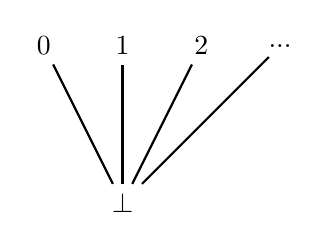
\begin{tikzpicture}
    \node (top) at (0,0) {$\bot$};
    \node (a) at (-1,2) {0};
    \node (b) at (0,2) {1};
    \node (c) at (1,2) {2};
    \node (d) at (2,2) {...};
    \draw [thick] (top) -- (a);
    \draw [thick] (top) -- (b);
    \draw [thick] (top) -- (c);
    \draw [thick] (top) -- (d);
\end{tikzpicture}
\end{center}

\vspace{0.5cm}

Now we must prove that this is a domain:

\vspace{0.5cm}

\begin{lem}
$(\mathbbm{N}, \bot, \sqsubseteq)$ is a domain.
\end{lem} 

\begin{proof}
We prove the three conditions in the domain definition:

In the definition of our relation we have $\{ (\bot , n) \ | \ n \in \mathbb{N} \}$ and $(\bot , \bot)$. so $\{(\bot , x) \ | \ x \in \natb\}$ is a subset of $\sqsubseteq$. Therefore $\forall x \in \natb. \ \bot \sqsubseteq x$.

Next, we prove $\sqsubseteq$ is a partial order. From the  definition of $\sqsubseteq$, as $\{(x,x) \ | \ x \in \natb \}$ is a subset of $\sqsubseteq$, so $\sqsubseteq$ must be reflexive.

We prove antisymmetry by case analysis. When $x = \bot$, the only possible $y$ we can have such that $y \sqsubseteq x$ is $y = \bot$, as  $n \sqsubseteq \bot$ is not defined in the relation for any $n$. Therefore $x = y = \bot$. When $x = n$, the only possible value of $y$ is $n$, so $x = y = n$. Therefore every element of the underlying set satisfies antisymmetry.

We also prove transitivity by case analysis. If $x = \bot$ and $y =n$, then we must have $z = n$ for $(y,z)$ to be in $\sqsubseteq$. Then we need $\bot \sqsubseteq n$ , which we have, as we have $(\bot, n)$, for any $n \in \mathbb{N}$, defined in the relation. If $x = \bot = y$, then we have two options for $z$. When $z = n$, we should have $\bot \sqsubseteq n$, which we have, as we have $(\bot, n)$ for any $n \in \mathbb{N}$ defined in the relation. When $z = \bot$, we just want $ \bot \sqsubseteq \bot$, which is also in the definition of $\sqsubseteq$. If $x = n$, then both $y$ and $z$ must also be equal to $n$ for $x \sqsubseteq y$ and $y \sqsubseteq z$ to be defined. Therefore we should  have $n \sqsubseteq n$. This is in the definition of $\sqsubseteq$.

Finally we prove that all chains must have a least upper bound. We prove this by case analysis on the different chains. For  chains of the form $\bot \sqsubseteq \dots \sqsubseteq \bot$, let $z = \bot$. The last element in the chain will always be $\bot$, so for every $i$ we have $\bot \sqsubseteq \bot$. Therefore $\forall i . x_i \sqsubseteq \bot$.
For the second statement, as every element is $\bot$, $x_i = \bot$ and $y = \bot$, we have $\bot \sqsubseteq \bot$ for $z \sqsubseteq y$. Therefore $\forall y. (\forall i . x_i \sqsubseteq y) \Rightarrow \bot \sqsubseteq y$ holds.

For chains of the form $n \sqsubseteq \dots \sqsubseteq n$, let $z = n$. The last element in the chain will always be $n$, so for every $n$ we have $n \sqsubseteq n$. Therefore $\forall i . x_i \sqsubseteq n$. For the second part, every element is $n$, so $x_i = n$ and $y = n$. Then we have $n \sqsubseteq n$ for $z \sqsubseteq y$. Therefore $\forall y. (\forall i . x_i \sqsubseteq y) \Rightarrow n \sqsubseteq y$ holds.

For chains of the form $\bot \sqsubseteq \dots \sqsubseteq \bot \sqsubseteq n \sqsubseteq \dots \sqsubseteq n$, let $z = n$.  The last element will be $n$. We have both $\bot \sqsubseteq n$ and $n \sqsubseteq n$ in the relation, so for any $x$, we have $x \sqsubseteq n$. Therefore $\forall i . x_i \sqsubseteq n$. For the second part, $(\forall i . x_i \sqsubseteq y)$ is only true when $y = n$, so we only have to consider this case. Then we have $n \sqsubseteq n$ for $z \sqsubseteq y$. Therefore $\forall y. (\forall i . x_i \sqsubseteq y) \Rightarrow n \sqsubseteq y$ holds.
\end{proof}

\subsection{Product of domains}\label{prod}
Given two domains $\mathbb{X} = (X, \bot_X, \sqsubseteq_X)$ and $\mathbb{Y} = (Y, \bot_Y, \leq_Y)$, we have a new domain,  where $X \times Y$ is the underlying set, the bottom element is $(\bot_X, \bot_Y)$ and $(x,y) \sqsubseteq (x',y')$ is defined when $x \sqsubseteq_X x'$ and $y \leq_Y y'$ are defined.

\vspace{0.25cm}

Now we must prove that this is a domain.

\vspace{0.5cm}

\begin{lem}
$(X \times Y, (\bot_X, \bot_Y), \sqsubseteq)$ is a domain
\end{lem}

\begin{proof}
We prove the three conditions in the domain definition:

As $\mathbbm{X}$ is a domain, we know $\forall x \in X. \ \bot_X \sqsubseteq_X x$ and because $\mathbb{Y}$ is a domain, we know $\forall y \in Y. \ \bot_Y \leq_Y y$. Therefore we have $\forall x,y . \ \bot_X \sqsubseteq_X x \wedge \bot_Y \leq_Y y$. This is the same as $\forall (x,y) \in X \times Y. (\bot_X,\bot_Y) \sqsubseteq (x,y)$.

Next, we prove $\sqsubseteq $ is a partial order. For an element $(x,y) \in X \times Y$, we have $x \sqsubseteq_X x$ and $y \leq_Y y$ because $\mathbb{X}$ and $\mathbb{Y}$ are domains, so their orderings are reflexive. This means we have $(x,y) \sqsubseteq (x,y)$, so $\sqsubseteq$ is also reflexive. For elements $(x,y)$ and $(x',y')$ we can assume $(x,y) \sqsubseteq (x',y')$ and $(x',y') \sqsubseteq (x,y)$. Expanding these definitions we have $x \sqsubseteq_X x' \wedge y \leq_Y y' \wedge x' \sqsubseteq_X x \wedge y' \leq_Y y$. If we reorder this we have:

\[x \sqsubseteq_X x' \wedge x' \sqsubseteq_X x \wedge y \leq_Y y' \wedge y' \leq_Y y \]

As the orderings on $\mathbb{X}$ and $\mathbb{Y}$ are antisymmetric, we can rewrite this as $x = x'$ and $y = y'$. Therefore we have $(x,y) = (x',y')$, so $\sqsubseteq$ is antisymmetric. For elements $(x,y), (x',y')$ and $(x'',y'')$ we can assume $(x,y) \sqsubseteq (x',y')$ and $(x',y') \sqsubseteq (x'',y'')$. Expanding these definitions gives us $x \sqsubseteq_X x' \ \wedge \ y \leq_Y y' \wedge \ x' \sqsubseteq_X x'' \wedge y' \leq_Y y''$. If we reorder this we have:


\[x \sqsubseteq_X x' \wedge x' \sqsubseteq_X x'' \wedge y \leq_Y y' \wedge y' \leq_Y y'' \]

As the orderings on $\mathbb{X}$ and $\mathbb{Y}$ are transitive, we can rewrite this as $x \sqsubseteq_X x''$ and $y \leq_Y y''$. Therefore we can now define $(x,y) \sqsubseteq (x'',y'')$, so $\sqsubseteq$ is transitive.

Finally we prove that all chains have a least upper bound. Chains of $\mathbbm{X \times Y}$ will be of the form:

\[(x,y) \sqsubseteq (x', y') \sqsubseteq (x'', y'') \sqsubseteq \dots \]

where $x \sqsubseteq_X x' \sqsubseteq_X x'' \dots$ and $y \leq_Y y' \leq_Y y'' \dots $.

Let $z = \bigsqcup (x, y)_n = (\bigsqcup x_n, \bigsqcup y_n)$. Then as $\mathbb{X}$ and $\mathbb{Y}$ are domains, we have $\forall i. \ x_i \sqsubseteq_X \bigsqcup x_n$ and  $\forall i. \  y_i \leq_Y \bigsqcup y_n$. Therefore, for any $(x,y)$ we have $\forall i. (x_i ,y_i) \sqsubseteq (\bigsqcup x_n , \bigsqcup y_n)$.

%\item{$\forall (x',y'). \ (\forall i . (x_i,y_i) \sqsubseteq (x',y')) \Rightarrow z \sqsubseteq (x',y')$\\
As $\mathbb{X}$ and $\mathbb{Y}$ are domains, we have $\forall x'. \  (\forall i.\  x_i \sqsubseteq_X x') \Rightarrow \bigsqcup x_n \sqsubseteq_X x'$ and $\forall y'. \ (\forall i. \ y_i \leq_Y y') \Rightarrow \bigsqcup y_n \leq_Y y'$.

 Therefore if we assume $\forall (x',y'). (\forall i . (x_i,y_i) \sqsubseteq (x',y'))$, then we know $\bigsqcup x_n \sqsubseteq_X x'$ and $\bigsqcup y_n \leq_Y y'$. This is the definition of $(\bigsqcup x_n , \bigsqcup y_n) \sqsubseteq (x',y')$.

\vspace{0.25cm}

Now we have proved all the conditions, so the product of two domains is also a domain.
\end{proof}

\section{Monotone and Continuous Functions}
There are two different types of functions that we will use when modelling PCF functions:

\vspace{0.25cm}

\begin{defn}
A \textbf{monotone} function, $f$, is a function that preserves the order of a partially ordered set, $X$,  so:

\[ \forall x, y \in X. \ x \sqsubseteq y  \Rightarrow f(x) \sqsubseteq f(y) \]
\end{defn}

Given a chain $x_0 \sqsubseteq x_1 \sqsubseteq \dots$, we can form the chain $f(x_0) \sqsubseteq f(x_1) \sqsubseteq \dots$ using a monotone function.

\vspace{0.25cm}

\begin{defn}
A \textbf{continuous} function $f$ is a function which when applied to the limit of a chain gives the same result as the limit of the chain formed by applying $f$ to every element of another chain. Formally:

\[ f(\bigsqcup x_n) = \bigsqcup (f(x_n))\]
\end{defn}

Therefore continuous functions must also be monotone:

\vspace{0.25cm}

\begin{thm}\label{mono}
Continuous functions are monotone
\end{thm}

\begin{proof}
Given a continuous function $f$, on a partially ordered set $X$, we need to show that $\forall x,y \in X. \ x \sqsubseteq y \Rightarrow f(x) \sqsubseteq f(y)$.
Assume we have a chain $x_n$, where $x_0 = x$ and $x_{n + 1} = y$ for all $n$:

\[x \sqsubseteq y \sqsubseteq y \dots \] .

The limit of this chain will be $y$, so $f(\bigsqcup x_n) = f(y) = \bigsqcup (f (x_n))$.

We also know that because there are only two different elements in the chain, $\bigsqcup (f (x_n)) = f(x) \sqcup f(y) = f(y)$, so therefore $f(x) \sqsubseteq f(y)$.

\end{proof}

\subsection{Domain of Continuous Functions}\label{cont}

We can form a domain of continuous functions between two other domains:

Given two domains, $\mathbb{X} = (X, \bot_X, \sqsubseteq_X)$ and $\mathbb{Y} = (Y, \bot_Y, \leq_y)$, we can form the set $\cont(X,Y) =\{ f : X \to Y\}$, of continuous functions between the underlying sets, where:

\begin{itemize}
\item{$\forall x, x' \in X. \ x \sqsubseteq_X x' \Rightarrow f(x) \leq_Y f(x')$ \hspace{1cm} $f$ preserves the ordering of chains in $\mathbbm{X}$}
\item{$x_n \in \chain(X) \Rightarrow f(\bigsqcup x_n) = \bigsqcup f(x_n)$ \hspace{2cm} $f$ is continuous}
\end{itemize} 

where $\chain(X)$ is the set of all possible chains we can form from  $\mathbbm{X}$.

$\bot_{X \to Y}$ is defined as the function $\bot = \lambda x. \bot (x)$, the function that loops on all inputs. The output of this function will always be $\bot$, because it does not terminate. 

The relation $\rel$ is defined as

\[ \rel  \ = \{ (f , g) \ | \ f,g \in \cont(X,Y) \ \wedge \ \forall x \in X. \ f(x) \leq_Y g(x)\} \]

Therefore our domain will be $(\cont(X,Y), \bot_{X \to Y}, \sqsubseteq_C)$. Now we must prove that this is a domain.

\vspace{0.5cm}

\begin{lem}
$(\cont(X,Y), \bot_{X \to Y}, \sqsubseteq_C)$ is a domain.
\end{lem}

\begin{proof}
We must prove the three conditions in the domain definition:

For all $x \in X$ we have $\bot \leq_Y f(x)$. As $\mathbb{Y}$ is a domain we know this holds for every element of $Y$ and as the codomain of $f$ is $Y$, every $f(x)$ is in $Y$. Therefore $f\forall f \in \cont(X,Y). \ \bot_{X \to Y} \rel f$.

Next we prove $\rel$ is a partial order. As $\mathbb{Y}$ is a domain, we know that $\leq_Y$ is a partial order. For reflexivity, we need to prove that $\forall f \in \cont(X,Y). \ f \rel f$. We can rewrite this using the definition of $\rel$ to get 
\[\forall f \in \cont(X,Y). \ (\forall x \in X. \ f(x) \leq_Y f(x))\]
 Functions are single valued, so we know $\forall f. \ \forall x. \ f(x) = f(x)$ and as $\leq_Y$ is reflexive we know $\forall f. \forall x \in X. \ f(x) \leq_Y f(x)$. Therefore we have $f \rel f$, for any $f \in \cont(X,Y)$. For antisymmetry, we need to prove that $\forall f,g \in \cont(X,Y). \ ((f \rel g) \ \wedge \ (g \rel f)) \Rightarrow f = g$. Rewriting this using the definition of $\rel$ gives us
 \[\forall f,g \in \cont(X,Y). \ (\forall x \in X. \ ((f(x) \leq_Y g(x)) \ \wedge \ (g(x) \leq_Y f(x))) \Rightarrow f(x) = g(x))\] 
 $\leq_Y$ is antisymmetric, so we have $\forall x \in X. \ f(x) = g(x)$, for any values of $f$ and $g$. Therefore $\rel$ is also antisymmetric. For transitivity, we need to prove that $\forall f,g,h \in \cont(X,Y). \ ((f \rel g) \  \wedge \ (g \rel h)) \Rightarrow f \rel h$. Rewriting this using the definition of $\rel$ gives us 

\[\forall f,g,h \in \cont(X,Y). \ (\forall x \in X. \ ((f(x) \leq_Y g(x)) \ \wedge \ (g(x) \leq_Y h(x))) \Rightarrow f(x) \rel h(x)) \]
 
As $\leq_Y$ is transitive, we have $\forall x \in X.f(x) \leq_Y h(x)$, for all $f, g$ and $h$. Therefore $\rel$ is also transitive. 

Finally we prove that all chains have a least upper bound. Let $z = \lambda x. \bigsqcup^Y f_n (x)$, where $\sqcup^Y f_n (x)$ is the limit of the chain (in $\mathbbm{Y}$) obtained by applying the functions in some chain of elements of $\cont(X,Y)$ to a certain element $x \in X$.

An example of a chain of such functions is:

\[ f_1 \rel f_2 \rel \dots \rel \bigsqcup f_n \]

If we expand this using the definition of $\rel$ we have

\[ \forall x \in X. \ (f_1(x) \leq_y f_2(x) \leq_Y \dots \leq_Y \bigsqcup f_n (x)) \]

This is a set of chains in $\chain(\mathbb{Y})$ where every chain contains the result of each function on a certain $x \in \mathbbm{X}$. As $\mathbb{Y}$ is a domain, the least upper bound is defined for any chain using the elements of $Y$. Therefore we know that the least upper bound $\bigsqcup f_n (x)$ is defined. Now we can see that this is the same as our definition of $z$, which was $\lambda x. \bigsqcup^Y f_i (x)$.

For the second part of the proof, we can rewrite it using the definition of $\rel$ as

\[ \forall x \in X. \ (\forall g. (\forall i . f_i(x) \leq_Y g(x)) \Rightarrow z(x) \leq_Y g(x)) \]


As $\mathbbm{Y}$ is  a domain, $(\forall i . f_i(x) \leq_Y g(x)) \Rightarrow z(x) \leq_Y g(x))$ holds for each of our individual chains for each $x \in X$. Therefore we have $ \forall g. (\forall i . f_i \rel g) \Rightarrow z \rel g$
\end{proof}


\section{Fixpoint Theorem}\label{fixpoint}

Now we have a domain of continuous functions, we can use it to state and prove the fixpoint theorem. The following theorem is an important result in recursion theory, that we will use to model recursion in PCF. The chain given in the theorem is the chain obtained by repeatedly iterating a recursive function on its previous result. If an input of the function is computed using $f^n(\bot)$ and it needs more than $n$ iterations then it will not terminate. As the chain can be infinitely long, it can model infinite (general) recursion.

\vspace{0.5cm}


\begin{thm}
Every continuous function $f : X \to X$ has a least fixpoint, which is the limit of the chain $\bot \sqsubseteq f(\bot) \sqsubseteq f^2(\bot) \sqsubseteq \dots$
\end{thm}

\begin{proof}
 Define the fixpoint function $fix(f) \equiv \bigsqcup f^n (\bot)$. This is the limit of the chain in the theorem. We know this limit exists because $f$ is continuous, so $(X, \bot, \sqsubseteq)$ must form a domain (see Section \ref{cont}), and by the definition of domain, all chains of $\mathbbm{X}$ have a limit. 

%First we must prove that this limit exists, so $\forall i \in \mathbb{N} . \ f^i(\bot) \sqsubseteq f^n(\bot)$. We prove this by induction. If $i = 0$, then the only element of the chain is $f^0(\bot) = \bot$. $\bot$ is the least element of the chain, so we have $\bot  \sqsubseteq f^n(\bot)$. 

%The inductive hypothesis is $\sqcup f^i(\bot)$ exists. Applying $f$ to this gives us $f(\sqcup f^i(\bot))$. $f$ is continuous, so this is equal to $\sqcup f(f^i(\bot)) = \sqcup f^{i+1}(\bot) $

\paragraph{$\bigsqcup f^n (\bot)$ is a fixpoint}
For the limit to be a fixpoint we must have  $f( \bigsqcup f^n (\bot)) =  \bigsqcup f^n (\bot)$.  As $f$ is continuous, we have $f( \bigsqcup f^n (\bot)) = \bigsqcup f(f^n(\bot)) = \bigsqcup f^{n+1}(\bot)$. The chain formed by $f^{n+1}$ is $f(\bot)  \sqsubseteq f^2(\bot) \sqsubseteq \dots$. This is the same as our original chain, but without $\bot$ at the start. Because $\mathbbm{X}$ is a domain, we know that $\forall x \in X. \ \bot \sqsubseteq x$. Therefore $\bot$ has no effect on the limit because every element is higher than it, so removing $\bot$ will not change the limit. This means that $\bigsqcup f^{n+1} (\bot) = \bigsqcup f^n(\bot)$.

\paragraph{$\bigsqcup f^n (\bot)$ is the least fixpoint}
Let $x$ be an element of our chain such that $fix(x) = x$. Then for $\bigsqcup f^n (\bot)$ to be the least fixpoint, we must have $\bigsqcup f^n (\bot) \sqsubseteq x$ (i.e.\ so $x$ is an upper bound that is higher than $\bigsqcup f^n (\bot)$). First we prove $x$ is an upper bound, so  we must show $\forall n. \ f^n(\bot) \sqsubseteq x$. We prove by this by induction on $n$:

if $n = 0$, then $f^0(\bot) \sqsubseteq x$, This is the same as $\bot \sqsubseteq x$, which is true because $\bot$ is the least element of the chain.

Our inductive hypothesis is $f^n(\bot) \sqsubseteq x$. As $f$ is continuous, $f$ is monotone, so $f(f^n(\bot)) \sqsubseteq f(x) = f^{n+1}(\bot) \sqsubseteq x$. Therefore we know that for any element $f^n(\bot)$ in the chain, $f^n(\bot) \sqsubseteq x$. 

As $\bigsqcup f^n (\bot)$ is a least upper bound, we know that  $\forall x \in X. \  \forall n. \ (f^n(\bot) \sqsubseteq x) \Rightarrow \bigsqcup f^n (\bot) \sqsubseteq x$. We have just proved the left hand side of this, so we now have $\bigsqcup f^n (\bot) \sqsubseteq x$.

\vspace{0.5cm}

Now we have proved that $\bigsqcup f^n (\bot)$ is the least fixpoint of $f$.
\end{proof}

Now that we have proved the above theorem, we know enough Domain Theory to model recursive PCF programs of any type.

\section{Logical Relations}\label{log}

Logical relations, developed in \citep{Tait67},\citep{Plotkin73},\citep{Statman85}, are a proof technique that is used for proving properties that cannot be proved by structural induction alone, due to higher order constructions being present in the structure we are proving a property of.

They have been used to prove Strong Normalisation (i.e.\ that every expression terminates) of systems such as the Simply Typed $\lambda$ Calculus, Type Safety and Program Equivalence.

\subsection{Definition}
We can define logical relations on program terms in PCF (or any other language) by defining relations on each type individually. We use Streicher's definition, as given in \citep{Streicher06}: 

\vspace{0.5cm}

\begin{defn}
Let $W$ be an arbitrary set.  A $W$-ary \textbf{logical relation} on the model of PCF is a family of relations

\[R = (R_A \in \mathcal{P}(\llbracket A \rrbracket^W) \ | \ A \in Type)\]

such that

\[f \in R_{A \to B} = \forall d \in R_A. \ \lambda i \in W. \ f(i)d(i) \in R_B\]
\end{defn}

where $Type$ is the set of all possible types our programs can have, defined by induction.

Different logical relations are defined by defining the relation differently on  the base type. For example, if the types are defined by the base type being $\nat$ and other types $A \to B$ (formed any other types $A$ and $B$), then the relation is defined by the definition of $R_{\nat}$.

Therefore we say that a logical relation $R$ of arity $W$ is uniquely determined by $R_{\nat}$, so for all subsets of ${\llbracket \nat \rrbracket}^W$ there is a unique $R$ equal to the set. 

\vspace{0.5cm}

\paragraph{Logical Relations at Function Types}

For a function $f = (f_1, \dots f_n)$ to be in the relation, if we apply it to \textbf{any} value that is in the relation of the type of its domain, for example, for arity $3$:

\[ (x,y,z) \in R_A \]

Then $f$ applied to everything in these elements will be in the relation of the codomain, so we must have:

\[ (f_1(x),f_2(y),f_3(z)) \in R_B \]

Then $f \in R_{A \to B}$.

%Define a set of types, $Type$, which is formed by:
%
%\[ \theta ::= o \ | \ \theta \to \theta \]
%
%such that $\llbracket o \rrbracket = X$ and  $\llbracket \theta_1 \to \theta_2 \rrbracket = \llbracket \theta_1 \rrbracket \to \llbracket \theta_2 \rrbracket$
%
%\begin{defn}
%An $n$-ary \textbf{logical relation} is a family $\mathcal{R} = \{R_\theta\}_{\theta \in Type}$ of $n$-ary relations such that $R_\theta \subseteq \llbracket \theta \rrbracket \times \dots \llbracket \theta \rrbracket$ (i.e.\ an $n$-tuple) for any $\theta$ and
%
%\[ R_{\theta_1 \to \theta_2}(f_1, \dots f_n) \Leftrightarrow\]
%
%
%for all $(d_1, \dots d_n) \in \llbracket \theta_1 \rrbracket^n$, if $R_{\theta_1}(d_1, \dots d_n)$ then $R_{\theta_2}(f_1(d_1), \dots f_n(d_n))$ 
%\end{defn}

\subsection{Examples and Non-Examples}


Applying certain restrictions on $R_{\nat}$ restricts the relations we can define on function types, for example:

\begin{itemize}
\item{If $R_{\nat} = \llbracket \nat \rrbracket^n$, relations on function types can only have $n$ arguments, if $n$ is specified, otherwise 
there is no difference to the definition.}
\item{If $R_{\nat} = \emptyset$, then all relations in $R$ are the empty relation.}
\end{itemize}

\paragraph{Union of two logical relations}
Given two logical relations $R$ and $S$ of the same arity, we could try to form a logical relation $R \cup S$. This is \textbf{not} a logical relation. For example, if we have $(f_1, \dots , f_n) \in R_{A \to B}$ (and not in $S_{A \to B}$) and $(d_1, \dots , d_n) \in S_A$, (and not in $R_{A \to B}$)  then $(f_1(d_n), \dots , f_n(d_n))$ cannot be in either $R$ or $S$.

\paragraph{Intersection of two logical relations}
Therefore if we restrict the logical relation to only contain tuples that are in both $R$ and $S$ then we do not have this problem, so this is a logical relation.

If the relations did not have the same arity, there will be no tuples that are in both relations that satisfy the definition, as if we have $R$ of arity 3 and $S$ of arity 5, then have, for example, $(f,g,h) \in R_{A \to B}$ and $(f,g,h,i,j) \in S_{A \to B}$, then we cannot say that $(f,g,h)$ is in both, as this would not be in $S$ anymore. Therefore, this would not be a logical relation.

\paragraph{Composition of two binary logical relations}
We define $R;S$ in the following way:

\[ (R;S)(x,y) \Leftrightarrow \exists z. \ (R(x,z) \ \wedge \ S(z,y))\]

So for base type we have:

\[ (R_{\nat};S_{\nat})(x,z) \Leftrightarrow \exists y. \ (R_{\nat}(x,y) \ \wedge \ S_{\nat}(y,z))\]

and for functions we have

\[ (R_{A \to B};S_{A \to B})(f,h) \Leftrightarrow \exists g. \ (R_{A \to B}(f,g) \ \wedge \ S_{A \to B}(g,h))\] 

where for any $(x,z) \in (R_A;S_A)$ we have

\[ (R_B(f(x),g(y)) \ \wedge \ S_B(g(y),h(z)))\] 

So as functions in $R$ are only applied to inputs that are in $R$ and the same for $S$, and functions in both are only applied to inputs that are in both, then \textbf{this is a logical relation.}  

\subsection{Main Lemma}
When using logical relations, we usually prove a general theorem about the relation, which we then give specific inputs to, to get the proof of our original property. This is called the Main Lemma (or sometimes the Fundamental Property/Theorem/Lemma). For program terms, we define the Main Lemma in the following way, as in \citep{Streicher06}. (Note that this definition uses the denotational semantics of PCF, so reading Chapter \ref{ch6} first will make this definition much easier to understand): 

\vspace{0.5cm}

For any denotation of a PCF term, we want to show that it is in the relation at its type, so we want to show that $\llbracket \Gamma \vdash e : A \rrbracket \in R_{\Gamma \to A}$. An element of $\llbracket \Gamma \rrbracket$ is any tuple of substitutions $d^* = (d_1, \dots d_n)$ for $x_1 : A_1, \dots x_n :A_n = \Gamma$. So $R_\Gamma \in \mathcal{P}(\llbracket A_1 \rrbracket \times \dots \times \llbracket A_n \rrbracket$).

We want all substitutions in a set of size $W$ to be in the relation, so using the definition of $f \in R_{\Gamma \to A}$, we want to show that 

\[ \forall d \in R_\Gamma. \ \lambda i \in W. \llbracket \Gamma \vdash e : A \rrbracket(d(i))\]

This says that for any position in the $W$-tuple, we have the denotation of $e$ using the substitution $d$ from the $i$th position in the $d \in R_\Gamma$.

For $W$ different substitutions we want to have

\[(\llbracket \Gamma \vdash e : A \rrbracket(d^*)_1 , \dots, \llbracket \Gamma \vdash e : A \rrbracket(d^*)_W) \in R_B \]

Therefore the main lemma \textcolor{red}{(for $\lambda terms??$)} is the following:

\vspace{0.5cm}

\begin{lem}\label{main2}
Let $R$ be a logical relation of arity $W$ on the Scott Model of PCF. Then for $\lambda$ terms $\Gamma \vdash e : A$ and $d_j \in R_{A_j}$ for $j = 1, \dots, n$

\[ \lambda i \in W. \llbracket \Gamma \vdash e : A \rrbracket(d^*(i)) \in R_A\]

where $d^*(i) = d_1(i) \dots d_n(i)$ and $\Gamma = x_1 : A_1 , \dots x_n : A_n$
\end{lem}

%\begin{lem}

%Let $\Gamma \vdash e : A$ where $\Gamma = \{x_1 : \theta_1, \dots x_m : \theta_m\}$ and $f = \llbracket \Gamma \vdash M : \theta \rrbracket$. Suppose $\{R_\theta\}$ is an $n$-ary logical relation and
%
%\[\gamma_i = (d_{i1} \dots d_{im}) \in \llbracket \theta_1 \rrbracket \times \dots \times \llbracket \theta_m \rrbracket\] 
%
%where $i = 1, \dots n$, are such that $R_{\theta_j}(d_{1j} \dots d_{nj})(1 \leq j \leq m)$. Then 
%
%\[R_\theta(f\gamma_1, \dots , f\gamma_n)\]  
%\end{lem}
%
%This says that for a well typed term $M$, that has a denotation equal to a function $f$, if we have a logical relation for types, then any possible set of substitutions for the variables in $\Gamma$ (of which there are $n$), that are in that term will be a tuple, $\gamma_i$, in the relation, and applying $f$ to each of these tuples gives another tuple that will be in the relation. The resulting tuple will contain the result of $f$ for each substitution.
%Definition.
%Exercises for Murawski's slides

\chapter{Definition of PCF and Syntax}\label{ch3}

Programming Computable Functions (PCF) is a programming language that is based on the Simply Typed $\lambda$ Calculus, with the addition of a "fix" operator, that allows us to write recursive functions using fixpoint recursion.

\section{Definition of PCF}

\subsection{Types}
There are some versions of PCF in different papers and books (such as \citep{Plotkin77}, \citep{Gunter92}) where some use Booleans and Natural Numbers for the base types. Here we just use Natural numbers, where $0$ represents false and any non zero number represents true. We define our types using the following grammar:\\

\[A ::= \nat \ | A \to B\] 

\subsection{Expressions}

The allowable expressions include variables (represented by $x$), a constant $z$ representing the number $0$, and a successor function $s(e)$, which takes any expression as input and returns its successor. 

$\case$ takes an expression $e$, which we assume is a numerical value. If $e$ is zero, we return an expression $e_0$, otherwise we have the successor of some value $x$ and we return the expression $e_S$.

Then we have function application, in which a function $e$ is applied to an expression $e'$, and $\lambda$-abstraction, which denotes a function $e$ that takes an input $x$ of type $A$.

Our last expression is the fixpoint expression, which takes a value $x$ as input to a larger function $e$.

The grammar for expressions is:

\[e ::=  \ x \ | \ z \ | \ s(e) \  |  \ \case \ (e, z \mapsto e_0 , s(x) \mapsto e_S) \ |\ e \ e' \  | \lambda x:A.e \ | \ \fix \ x:A . \ e\]

\section{Type System for PCF}
$\Gamma$ is an example of a typing context, which is a function that maps variables to their types. For example, if we have an expression $x : A$ in the context, then $\Gamma(x) = A$. We write $\Gamma \vdash e : A$ for the context associated with an expression $e$ of type $A$.

Therefore we need a typing rule for each expression in PCF, which if satisfied means that we are allowed to write that expression. The typing rules are given as inference rules, where our assumptions are above the line and the conclusion underneath:

$$
\inferrule [variables]{ \Gamma(x) = A }
 {\Gamma \vdash x : A}
\hspace{1cm}
\inferrule [zero]{ \ }
 {\Gamma \vdash z : \nat}
\hspace{1cm}
\inferrule [succ]{ \Gamma \vdash e : Nat }
 {\Gamma \vdash s(e) : \nat}
$$

For \emph{variables}, if $x$ is in the domain of $\Gamma$, then we can conclude that we have a variable of that type.

$z$ is a constant, so it needs no assumptions.

For \emph{successor}, we must have an expression $e$ of type $\nat$ that we can apply the successor function to. We then know we have $s(e)$ of type $\nat$.

$$
\inferrule [case]{\Gamma \vdash e : \nat \\  \Gamma \vdash e_0 : A \\  \Gamma , x:\nat\vdash e_S : A}
  {\Gamma \vdash \ \case \ (e, z \mapsto e_0 , s(x) \mapsto e_S) \  : A}  
$$

For $\case$, we must have an expression $e$ of type $\nat$ to evaluate. Then we must have some other expressions $e_0$ and $e_S$ to return, which can be of any type, as long as they are the same type. As the condition of $e_S$ contains a specific $x$ value, we must also know that this is well typed. Therefore we add $x : \nat$ to the context of $e_S$.

$$
\inferrule [application]{\Gamma \vdash e : A \to B \\  \Gamma \vdash e' : A}
  {\Gamma \vdash e \ e' : B}
  \hspace{1cm}
\inferrule [abstraction] {\Gamma , x : A \vdash  e : B}
  {\Gamma \vdash \lambda x : A. e : A \to B}  
$$

For application, $e$ must have a function type and $e'$ must have the same type as the domain of $e$. Then we can apply $e$ to $e'$ to get the expression $e \ e'$ of the type of the codomain of $e$.

For $\lambda$ abstraction, we need an expression $e$ of some type $B$ and we must know that the parameter $x$ is in the context of this expression, to be able to use it in the $\lambda$ abstraction. Then in the conclusion, as $x$ is now bound to the expression, we remove it from the context of $B$.

$$
\inferrule [fix]{\Gamma, x : A \vdash e : A }
  {\Gamma \vdash \  \fix \ x:A . \ e : A}
$$

The fixpoint case is exactly the same as $\lambda$ abstraction, where the $x$ is bound to the fixpoint expression.

\vspace{0.5cm}

For any well typed PCF expression, we can obtain a derivation tree, where the root is the whole expression and the branches go up until we end up with the variables and constants of the expression at the leaves.

We also note that given a typing context $\Gamma$, an expression $e$ and a type $A$ such that we have the typing judgement $\Gamma \vdash e : A$, there is only one possible derivation of this judgement.

\chapter{Operational Semantics of PCF}\label{ch4}
Now we have defined the syntax and typing rules of PCF, we can use this to define its operational semantics.

We use the \textbf{Call By Name} evaluation strategy, which means that function arguments are placed into the body of the function and evaluated within the entire function's evaluation, instead of before.

The semantics we define are \textbf{small step} semantics, which means that in $e \mapsto e'$, the transition relation $\mapsto$ must take an expression $e$ to another expression $e'$ in only one step.

The first rules we have are \textbf{congruence rules}, which use the assumption $e \mapsto e'$ to replace $e$ with $e'$ in the whole expression. We can define these rules for any PCF expression that has an expression as a parameter, so this will be function application, successor and case:

$$
\inferrule { e_0 \mapsto e_0'} {e_0 \ e_1 \mapsto e_0' \ e_1}
\hspace{1cm}
\inferrule { e \mapsto e'} {s(e) \mapsto s(e')}
$$

$$
\inferrule { e \mapsto e'} {\case \ (e, z \to e_0 , s(x) \to e_S) \mapsto \case \ (e', z \to e_0 , s(x) \to e_S)}
$$

(Note that we could have given the typing contexts before each expression in the evaluation rules, but as they do not change, we can omit them. The same is also true for the rest of the rules we define below.) 

Then we define rules on individual expressions. Note that the case rule above was only defined on expressions that reduce. The one defined below is only defined for \textbf{values}, which are expressions that have no applicable evaluation rule (including zero, successors of values, and lambda abstractions). This ensures that there is only one possible rule to apply to any expression.



$$
\inferrule{ \ }
 {(\lambda x: A .\ e) \ e' \mapsto [e'/x]e}
$$

The above rule states that given a function application, where the function is defined by a $\lambda$-abstracttion, we substitute $e'$ for $x$ in the expression $e$. This means that we replace every occurrence of $x$ in $e$ with the expression $e'$.

$$
\inferrule{ \ }
{\case \ (z, z \to e_0 , s(x) \to e_S) \mapsto e_0}
$$
$$
\inferrule{ \ }
{\case \ (s(v), z \to e_0 , s(x) \to e_S) \mapsto [v/x]e_S}
$$

The above rules give the evaluation of case, when we have a value as the condition expression. The first rule states that if $e = z$, then our result will be $e_0$. If $e = s(v)$, our result is $e_S$ , but we must also substitute $v$ for $x$ in $e_S$ (as $e_S$ is defined for a bound variable $x$, which we now know is equal to $v$).

$$
\inferrule{ \ }
{\fix \ x:A. e \mapsto [\fix \ x:A. e/x]e}
$$

The above rule states that we replace the bound variable $x$ in the expression $e$ with the entire fixpoint expression. This replaces a parameter in $e$, which should be the recursive call, with the contents of the function, so that we can evaluate it all again. Then when we get to that point in the new evaluation, we will replace $x$ with the whole expression. We can keep doing this infinitely, and keep expanding the evaluation in the following way:

\[ \fix \ x:A. e \mapsto [\fix \ x:A. e/x]e \mapsto 
[[\fix \ x:A. e/x]e/x]e
\mapsto
[[[\fix \ x:A. e/x]e/x]e/x]e \dots \]

We give an example of a function that uses the fixpoint operator in the following section.

\section{Example of a program in PCF}

\subsection{Addition}

In functional languages, we usually define mathematical operators on numbers as recursive functions. For example addition is the following function:

\[\add  0 \ y = y \]
\[\add  s(n) \ y = s(\add  n \ y)\]

We can write this as a $\lambda$ abstraction:

\[ \add = \lambda x,y : \nat. \ \case \ (x, z \mapsto y, s(v) \mapsto s(\add \ v \ y))\]

This is a recursive function, so to define it in PCF, it must be the fixpoint of some other function $A$:

\[ A = \lambda f: Nat \to Nat \to Nat. \ \lambda x,y : \nat. \ \case \ (x, z \mapsto y, s(v) \mapsto s(f \ v \ y))\]

Therefore we can define this in PCF as:

\[ \add x \ y = (\fix f : \nat \to \nat \to \nat . \ A : \nat \to \nat \to \nat) \ x \ y  \].

When we try to evaluate this term, we get the following, by the evaluation rule for $\fix$:

$\fix f : \nat \to \nat \to \nat . \ A : \nat \to \nat \to \nat = [\fix f : \nat \to \nat \to \nat . \ A : \nat \to \nat \to \nat/f]A$. This expands to:

\[ \lambda x,y : \nat. \ \case \ (x, z \mapsto y, s(v) \mapsto \]
\[s((\fix f: \nat \to \nat \to \nat . \ A : \nat \to \nat \to \nat) \ v \ y)) \]

Therefore expanding this infinitely gives all possible executions of the addition function.

%\end{document}



\chapter{Type Safety}\label{safe}
Type Safety is an important property of a programming language, as it proves that well typed programs do not go wrong. It is usually expressed as a property of the operational semantics, which we have defined in the previous chapter (see Chapter \ref{ch4}), and follows from the conclusion of two other lemmas we will prove; Type Preservation (\ref{pres}) and Type Progress (\ref{prog})

\section{Lemmas for Type Safety}
There are two simple lemmas we must prove which will aid us in proving the lemmas of Type Safety:

%Another assumption is that if $x:A$ is in $\Gamma$ and we add $x:C$ to $\Gamma$, then the type of $x$ is overwritten?

\subsection{Weakening}\label{weak} 
Weakening is the following theorem, which says that for an expression of type $A$ in a context $\Gamma$, adding another variable $x$ (of any type) to the context will not change the type of the expression:

\vspace{0.5cm}

\begin{thm}
If $\Gamma \vdash e:A$ then  $\Gamma,x:C \vdash e:A$ 
\end{thm}
 
\begin{proof}
We prove this theorem by induction on derivation trees, so if we have a derivation tree for our assumption then there exists a derivation tree for the conclusion.% We can use the inductive hypothesis

%\[ \Gamma \vdash e : A \Rightarrow \Gamma , x : C \vdash e : A \]


As there is only one derivation for a given judgement $\Gamma \vdash e : A$, we can use induction on the possible expressions:

\paragraph{Variables} We rename $x$ to $y$ using $\alpha$ equivalence. We assume $\Gamma \vdash y : A$, giving us the following derivation tree:

$$
\inferrule{\Gamma(y) = A}{\Gamma \vdash y : A}
$$ 

of which $\Gamma(y) = A$ is a subtree. $\Gamma$ is a function, so can also be represented by a set of (variable, type) pairs. Therefore $\Gamma, x: C$ is the set $\Gamma \ \cup \{(x,C)\}$. Therefore we define the function $(\Gamma,x:C)$, where $(\Gamma,x:C)(y) = A$ and for any other variable $z$, $(\Gamma, x:C)(z) = \Gamma(z)$. Then we just use the typing rule for variables to get the following derivation tree:

$$
\inferrule{(\Gamma, x : C) (y) = A}{\Gamma, x : C \vdash y : A}
$$ 

Now we have the required derivation tree, so weakening holds for variables.

\paragraph{Zero} We assume $\Gamma \vdash z : \nat$, giving us the following derivation tree:
$$
\inferrule{ \ }{\Gamma \vdash z : \nat}
$$.
The typing rule for zero says that no matter what $\Gamma$ is, we always have zero, because there are no assumptions. Therefore we can have $\Gamma, x: C$ as the context and get the following derivation tree:
$$
\inferrule{ \ }{\Gamma,x :C \vdash z : \nat}
$$

Now we have the required derivation tree, so weakening holds for zero.

\paragraph{Successor} We assume $\Gamma \vdash s(e) : \nat$, giving us the following derivation tree from the typing rule:
$$
\inferrule{\Gamma \vdash e : \nat}{\Gamma \vdash s(e) : \nat}
$$.

where $\Gamma \vdash e : \nat$ is a subtree. We can use the inductive hypothesis of weakening on this subtree to get $\Gamma , x : C \vdash e : \nat$. Then we use the typing rule for successor to get the following derivation tree:

$$
\inferrule{\Gamma, x : C \vdash e : \nat}{\Gamma, x : C \vdash s(e) : \nat}
$$.

Now we have the required , so weakening holds for the successor function.

\paragraph{Case} We assume $\Gamma \vdash \ \case \ (e, z \mapsto e_0 , s(y) \mapsto e_S) : A$, (renaming $x$ to $y$ using alpha equivalence) giving us the following derivation tree from the typing rule:

$$
\inferrule{\Gamma \vdash e : Nat \\  \Gamma \vdash e_0 : A \\  \Gamma , y:\nat \vdash e_S : A}
  {\Gamma \vdash \ \case \ (e, z \mapsto e_0 , s(y) \mapsto e_S) \  : A}  
$$

giving us the subtrees $\Gamma \vdash e : \nat$, $\Gamma \vdash e_0 : A$ and $\Gamma, y : \nat \vdash e_S : A$ from the assumption of the typing rule. Using the inductive hypothesis on each of these, we get $\Gamma, x : C \vdash e : \nat$, $\Gamma, x : C \vdash e_0 : A$ and $\Gamma, y : \nat , x : C \vdash e_S : A$, so we can use the typing rule again with these assumptions:

$$
\inferrule{\Gamma, x : C \vdash e : Nat \\  \Gamma, x : C \vdash e_0 : A \\  \Gamma, x : C , y:\nat\vdash e_S : A}
  {\Gamma, x : C \vdash \ \case \ (e, z \mapsto e_0 , s(y) \mapsto e_S) \  : A}  
$$

Now we have the required derivation tree, so weakening holds for the case expression.
 
\paragraph{Application} We assume $\Gamma \vdash e_0 \ e_1 : B$, giving us the following derivation tree:

$$
\inferrule{\Gamma \vdash e_0 : A \to B \\ \Gamma \vdash e_1 : A}{\Gamma \vdash e_0 \ e_1 : B}
$$

which gives us the subtrees $\Gamma \vdash e_0 : A \to B$ and $\Gamma \vdash e_1 : A$. Using the inductive hypothesis on these trees gives us $\Gamma, x : C \vdash e_0 : A \to B$ and $\Gamma, x : C \vdash e_1 : A$, so we can just use the typing rule for application again to get the following derivation tree:

$$
\inferrule{\Gamma, x :C \vdash e_0 : A \to B \\ \Gamma, x: C \vdash e_1 : A}{\Gamma, x : C \vdash e_0 \ e_1 : B}
$$

Therefore weakening holds for function application.


\paragraph{Abstraction} We rename $x$ to $y$ using $\alpha$ equivalence. We assume $\Gamma \vdash \lambda y : A. \ e : B$, giving us the following derivation tree:

$$
\inferrule{\Gamma, y : A \vdash e : B}{\Gamma \vdash \lambda y : A. \ e : A \to B}
$$

which gives us the subtree $\Gamma , y:A \vdash e : B$. Using the inductive hypothesis, we get $\Gamma , y:A , x : C \vdash e : B$. Then we use the typing rule for $\lambda$ abstraction to get the following tree:

$$
\inferrule{\Gamma, y : A, x : C \vdash e : B}{\Gamma, x : C \vdash \lambda y : A. \ e : A \to B}
$$

Now we have the required derivation tree, so weakening holds for $\lambda$ abstraction.
 

\paragraph{Fixpoint}
 
We assume $\Gamma \vdash \fix \ y :A. \ e: A$, renaming $x$ to $y$ using $\alpha$ equivalence. This gives us the following derivation tree:

$$
\inferrule{\Gamma, y:A \vdash e : A}{\Gamma, y : A \vdash \fix \ y : A. \ e : A}
$$

As we have the subtree $\Gamma, y:A \vdash e : A$, we use the inductive hypothesis on this to get $\Gamma, x :C, y:A. \vdash e : A$. Then we use the typing rule for fix to get the following tree:

$$
\inferrule{\Gamma, x : C, y:A \vdash e : A}{\Gamma, x : C, y : A \vdash \fix \ y : A. \ e : A}
$$

Therefore weakening holds for the fixpoint operator. Now we have proved weakening for derivation trees of any expression so weakening always holds.


\end{proof}


\subsection{Substitution Rules} 
Next we want to prove a lemma that shows that substitutions preserve the intended type of a given PCF expression.

But before we prove this, we must actually define rules for substitution on the level of each possible expression that can be formed in PCF, which are all instances of $[e/x]e'$. This notation says that an expression $e$ replaces a variable $x$ in another expression $e'$.

When defining the substitution rules, we must be careful  that we avoid \textbf{variable capture} by bound variables. For example, given the following substitution:

\[ [s(x)/y](\lambda x. x + y) \]

if we naively substitute $s(x)$ for $y$ in $\lambda x. x + y$, we get $\lambda x. \ x + s(x)$ and the value of $x$ is now the value assigned to the bound $x$. Therefore we can use \textbf{renaming} to avoid this. 

\paragraph {Variables} There are two cases for substitution in variables. The first is for when $e'$ is the same as the variable being replaced:
\[[e/x]x = e\]
The second one is when $e$ is a completely different variable, for which nothing happens:
\[ [e/x]y = y\]

\paragraph{Zero} For zero, any substitution will have no effect, as zero is a constant:
\[ [e/x]z = z\]

\paragraph{Successor} The successor function cannot be changed, so we substitute $e$ in its argument:
 \[[e/x]s(e') = s([e/x]e')\]
 
\paragraph{Case} As we cannot change the case statement, we could substitute $e$ in the expressions given as arguments to the case statement, in the following way: 

\[ [e/x] \ (\case \ (e', z \mapsto e_0, s(x) \mapsto e_S)) = \case \ ([e/x]e', z \to [e/x]e_0, s(x)  \to [e/x]e_S)\]

But we must be careful with variable capture, as the derivation of $e_S$ is $\Gamma, x:Nat \vdash e_S$. If we have $[s(x)/y] e_S$ and $e_S = x + y$, then we have $x + s(x)$ and the value of $s(x)$ is bound by $\Gamma, x : Nat$. Therefore we should rename $s(x)$ in the case statement to something that is not free in $e_S$.

Therefore our rule for case will be:

\begin{minipage}{4in}
\begin{align*}
\intertext{$(\case \ (e', z \to e_0, s(x) \to e_S))=$}
  \begin{cases}
            (\case \ ([e/x]e', z \mapsto [e/x]e_0, s(x) \mapsto [e/x]e_S)) & \text{if } x \notin FV(e')  \\
            (\case \ ([e/x]e', z \mapsto [e/x]e_0, s(y) \mapsto [e/x]e_S)) & \text{if } x \in FV(e')
  \end{cases}
\end{align*} 
\end{minipage}

where $y \notin FV(e')$. 

For some expression $e$, $FV(e)$ is the set of free variables it contains.

\paragraph{Application} We substitute $e$ in the function and its argument, then apply the new function to the new argument:

\[ [e/x] (e_0 \ e_1) = [e/x]e_0 \ ([e/x]e_1) \]

\paragraph{$\lambda$ Abstraction} There are two cases, the first when the bound variable is $x$. This does nothing, as we are just rewriting the function using alpha equivalence in this case:
\[ [e/x](\lambda x:A. \ e') = \lambda x:A. \ e' \]
The second case is when the bound variable is not equal to $x$, where we substitute $e$ in the expression. If $y$ is a free variable in $e'$ then we must rename the bound variable to something else:

\begin{minipage}{4in}
\begin{align*}
\intertext{$[e/x](\lambda y:A.e')=$}
  \begin{cases}
            \lambda y:A. [e/x]e' & \text{if } y \notin FV(e')  \\
           \lambda z:A. [e/x]([z/y]e') & \text{if } y \in FV(e')
  \end{cases}
\end{align*} 
\end{minipage}

where $z \notin FV(e')$.

\paragraph{Fixpoint} Fixpoint is similar to $\lambda$ abstraction, so we have two cases. The first case is when the bound variable is $x$, for which we just rewrite the function using $\alpha$ equivalence. Therefore this rule does nothing:
\[ [e/x] \fix \ x:A. e' = \fix \ e:A. e'\]
When the bound variable is not equal to $x$, we substitute $e$ in the expression $e'$. If $y$ is a free variable in $e'$ then we must rename the bound variable to something else:

\begin{minipage}{4in}
\begin{align*}
\intertext{$[e/x](\fix \ y:A.e')=$}
  \begin{cases}
            \fix \ y:A. [e/x]e' & \text{if } y \notin FV(e')  \\
           \fix \ z:A. [e/x]([z/y]e') & \text{if } y \in FV(e')
  \end{cases}
\end{align*} 
\end{minipage}

where $z \notin FV(e')$.

\subsection{Substitution}

Now we have all the rules, we can prove Substitution, which is the following theorem. It says that if we have an expression $e$ that is well typed in the context $\Gamma$ and an expression $e'$ that is well typed in the context $\Gamma,x:A$, then the expression obtained by substituting $e$ for $x$ in $e'$ will be derivable in the context $\Gamma$:

\vspace{0.5cm}

\begin{thm}If $\Gamma \vdash e:A$ and $\Gamma, x:A \vdash e' : C$ then $\Gamma \vdash [e/x] e' : C$ \end{thm}

\begin{proof}
We can slso prove this by induction on derivation trees. %We can rewrite the theorem as "If $D :: \Gamma \vdash e:A$ and $E :: \Gamma, x:A \vdash e' : C$ then $F ::\Gamma \vdash [e/x] e' : C$, where $D$, $E$ and $F$ are derivation trees for each of the well typed terms. We use induction on the tree $E$, as we are interested in the possible expressions $e'$ could be. We can use the inductive hypothesis:

%\[(\Gamma \vdash e:A \ \wedge \Gamma, x:A \vdash e' : C) \Rightarrow \ \Gamma \vdash [e/x] e' : C\]

As there is only one derivation for a given judgement $\Gamma \vdash e : A$, again we can use induction on the possible values of $e'$:

\paragraph{Variables} We assume derivation trees exist for $\Gamma \vdash e : A$ and $\Gamma, x : A \vdash y : C$. As $y$ has a different type to $x$, it cannot be equal to it, so there is only one case, as we can only use one of the substitution rules. The tree for $y$ that is given is:

$$\inferrule{(\Gamma,x:A)(y) = C}{\Gamma, x:A \vdash y : C}$$

The function $\Gamma$ is the set of pairs $(\Gamma,x:A)\backslash \{(x,A)\}$. As $x:A$ does not affect the value of $y$, we will still have $\Gamma(y) = C$. Using the typing rule for variables, we get the tree:

$$\inferrule{\Gamma(y) = C}{\Gamma \vdash y : C}$$

$\Gamma \vdash y : C$ will be the same as $\Gamma \vdash [e/x]y : C$ using the substitution rule for variables, so we have the derivation tree needed. Therefore variables satisfy substitution.  

\paragraph{Zero} We assume derivation trees exist for $\Gamma \vdash e : A$ and $\Gamma, x : A \vdash z : \nat$. As $z$ is a constant, it exists in any context $\Gamma$, so we have a tree for $\Gamma \vdash z : \nat$. This is equal to $\Gamma \vdash [e/x]z : \nat$, as this is always zero no matter what $e$ and $x$ are. Therefore as we already have the tree for $\Gamma \vdash z : \nat$, we use it as the derivation tree for $\Gamma \vdash [e/x]z : \nat$.

\paragraph{Successor} We assume derivation trees exist for $\Gamma \vdash e : A$ and $\Gamma, x:A \vdash s(e') : \nat$. The second tree is the following:

$$\inferrule{\Gamma, x:A \vdash e' : \nat}{\Gamma, x:A \vdash s(e') : \nat}$$

Therefore we have a subtree $\Gamma, x:A \vdash e' : \nat$. Using the induction hypothesis on this and $\Gamma \vdash e : A$, we have a derivation tree for $\Gamma \vdash [e/x]e' : \nat$. Using the typing rule for successor on this gives us the following tree:

$$\inferrule{\Gamma \vdash [e/x]e' : \nat}{\Gamma \vdash s([e/x]e') : \nat}$$

Using the substitution rule for successor, we know the bottom half is equal to $[e/x]s(e')$, so we get the following derivation tree:

 $$\inferrule{\Gamma \vdash [e/x]e' : \nat}{\Gamma \vdash [e/x]s(e') : \nat}$$
 
which is a derivation tree for $\Gamma \vdash [e/x]s(e') : \nat$. Therefore substitution holds for successor function.

\paragraph{Case} We rename $x$ to $y$ using alpha equivalence, then assume derivation trees exist for $\Gamma \vdash e : A$ and $\Gamma, x: A \vdash \case \ (e', z \mapsto e_0 , s(y) \mapsto e_S) \  : C$. The second derivation tree gives us the subtrees $\Gamma, x:A \vdash e' : \nat$, $\Gamma, x : A \vdash e_0 : C$ and $\Gamma, y:Nat, x : A \vdash e_S : C$. Using the induction hypothesis and the tree for $\Gamma \vdash e : A$, we get  $\Gamma \vdash [e/x]e' : \nat$ and $\Gamma \vdash [e/x]e_0 : C$.

For $\Gamma, y:\nat, x : A \vdash e_S : C$, we need  to change the context of $e$ before we can apply the inductive hypothesis. We do this using our  Weakening Lemmma we just proved (in Section \ref{weak}), which gives us $\Gamma, y:\nat \vdash e : A$. Now we apply the inductive hypothesis with this to get $\Gamma, y:\nat \vdash [e/x]e_S : C$.
 
 
Now we can apply the typing rule to these trees to get the following derivation tree:

$$\inferrule{\Gamma \vdash [e/x]e' : \nat \\  \Gamma \vdash [e/x]e_0 : C \\  \Gamma , y:\nat \vdash [e/x]e_S : C}  {\Gamma \vdash \ \case \ ([e/x]e', z \mapsto [e/x]e_0 , s(y) \mapsto [e/x]e_S) \  : C}  
$$

By the substitution rule for case, we can replace the bottom half of the tree with $\Gamma \vdash [e/x] \ \case \ (e', z \mapsto e_0 , s(y) \mapsto e_S) \  : C$. Therefore substitution holds for the case statement. 

\paragraph{Application} We assume derivation trees exist for $\Gamma \vdash e : A$ and $\Gamma, x : A \vdash e_0 \ e_1 : C$. The second tree is the following:

$$
\inferrule{\Gamma , x:A \vdash e_0 : B \to C \\  \Gamma ,x:A \vdash e_1 : B}
  {\Gamma, x : A \vdash e_0 \ e_1 : C}$$

which contains the subtrees $\Gamma, x:A \vdash e_0 : B \to C$ and $\Gamma, x:A \vdash e_1 : B$. Combining each of these trees with $\Gamma \vdash e : A$ and the inductive hypothesis gives us $\Gamma \vdash [e/x]e_0 : B \to C$ and $\Gamma \vdash [e/x]e_1 : B$. Using the typing rule for function application with these trees gives us a derivation tree for $\Gamma \vdash [e/x]e_0 ([e/x]e_1) : C$. This is equal to $\Gamma \vdash [e/x](e_0 \ e_1) : C$, so we have the derivation tree for this judgement.

Therefore substitution holds for function application.

\paragraph{Abstraction} We rename $x$ to $y$ using $\alpha$ equivalence. Then derivation trees exist for $\Gamma \vdash e : A$ and $\Gamma, x : A \vdash \lambda y : B. \ e' : B \to C$. For the second tree we have the following:

$$\inferrule{\Gamma, x : A, y : B \vdash e' : C}{\Gamma, x:A \vdash \lambda y:B. \ e' : B \to C}$$

which gives us the subtree $\Gamma, x : A, y : B \vdash e' : C$. Then we use weakening on $\Gamma \vdash e : A$ to get $\Gamma, y : B \vdash e : A$
, which when used with the inductive hypothesis gives us $\Gamma, y : B \vdash [e/x]e' : C$. 


Applying the typing rule for $\lambda$ abstraction to this gives us the following tree:

$$\inferrule{\Gamma, y : B \vdash [e/x]e' : C}{\Gamma \vdash \lambda y:B. \ [e/x]e' : B \to C}$$.

Now there are two cases:

\begin{enumerate}
\item{When $y \notin FV(e')$, the substitution rule gives us $\lambda y:B. \ [e/x]e' = [e/x]\lambda y:B. \ e'$, so we have a derivation tree for $\Gamma \vdash [e/x]\lambda y:B. \ e' : B \to C$}
\item{When $y \in FV(e')$, rewrite $\lambda y:B. \ [e/x]e' : B \to C$ as $\lambda z:B. [e/x]([z/y]e')$. Then this is the same as $[e/x]\lambda y:B. \ e'$ , so we have a derivation tree for $\Gamma \vdash [e/x]\lambda y:B. \ e' : B \to C$} 
\end{enumerate} 


\paragraph{Fixpoint} We rename $x$ to $y$ using alpha equivalence, then assume derivation trees exist for $\Gamma \vdash e : A$ and $\Gamma, x : A \vdash \fix \ y:C. \ e' : C$. The second tree is the following:


$$\inferrule{\Gamma, y:C, x:A \vdash e' : C}{\Gamma,x:A \vdash \fix \ y:C. e' : C}$$

giving us the subtree $\Gamma, y:C, x:A \vdash e' : C$. Then we use weakening on $\Gamma \vdash e : A$ to get $\Gamma, y : C \vdash e : A$, which when used with the inductive hypothesis gives us $\Gamma, y:C \vdash [e/x]e' : C$. 

Applying the typing rule for fixpoint to this gives us the following derivation tree:

$$\inferrule{\Gamma, y:C \vdash [e/x]e' : C}{\Gamma\vdash \fix \ y:C. [e/x]e' : C}$$

Now there are two cases:

\begin{enumerate}
\item{When $y \notin FV(e')$, the substitution rule for fixpoint gives us $\Gamma\vdash \fix \ y:C. [e/x]e' : C = \Gamma \vdash [e/x](\fix \ y:C. e') : C$, so we have the required derivation tree and substitution holds for fixpoint.}
\item{When $y \in FV(e')$, rewrite $\fix \  y:C. \ [e/x]e' : C$ as $\fix \ z:C. [e/x]([z/y]e')$. Then this is the same as $[e/x]\fix \  y:C. \ e'$ , so we have a derivation tree for $\Gamma \vdash [e/x]\fix \  y:C. \ e' : C$}
\end{enumerate}


Now we have proved substitution holds for derivation trees of any expression $e'$.
\end{proof}

\section{Type Safety}
Now we can prove the two lemmas that form the property of Type Safety.

\subsection{Type Preservation} \label{pres}
Type preservation says that if an expression $e$ of type $A$ is well typed in a context $\Gamma$, and it evaluates in one step to $e'$, then $e'$ will also have type $A$ in $\Gamma$ (i.e.\ we get the same type at the end of the evaluation as we had at the start):
\vspace{0.5cm}

\begin{thm}
 If $\Gamma \vdash e:A$ and $e \mapsto e'$, then $\Gamma \vdash e' : A$
\end{thm}

\begin{proof}
We can prove this by induction on derivation trees.%, so we rewrite the theorem as "If $D :: \Gamma \vdash e:A$ and $E ::e \mapsto e'$ (in one step) then $\exists. F :: \Gamma \vdash e' : A$:

There will be a derivation tree  for each rule in the operational semantics, so we can check this statement for every evaluation rule on every possible expression:

\paragraph{Variables} There are no rules in the operational semantics for when $e$ is just a variable so we do nothing here.

\paragraph{Zero} Same as for variables.

\paragraph{Successor} We  assume $\Gamma \vdash s(e) : \nat$, so we have the following tree (by the typing rule of successor):

$$
\inferrule { \Gamma \vdash e : \nat }
 {\Gamma \vdash s(e) : \nat}
$$

Then we assume $s(e) \mapsto s(e')$, so we have the following tree, using the congruence rule for successor:
$$
\inferrule { e \mapsto e'} {s(e) \mapsto s(e')}
$$

From these two trees, we get the subtrees $\Gamma \vdash e : \nat$ and $e \mapsto e'$. Using the inductive  hypothesis of type preservation we get a tree for $\Gamma \vdash e' : \nat$. Then using the typing rule for successor with this we get a tree for $\Gamma \vdash s(e') : \nat$. 

There are no other rules when the expression is $s(e)$, so type preservation holds for successor expressions.  

\paragraph{Case} There are three evaluation rules, which depend on the expression $e$ being checked:

\begin{enumerate}
\item{If $e$ can be reduced, then we have the following tree from the typing rule for case:

$$
\inferrule{\Gamma \vdash e : \nat \\  \Gamma \vdash e_0 : A \\  \Gamma , x:\nat\vdash e_S : A}
  {\Gamma \vdash \ \case \ (e, z \mapsto e_0 , s(x) \mapsto e_S) \  : A}  
$$


and our second assumption uses the congruence evaluation rule for case as:

$$
\inferrule { e \mapsto e'} {\case \ (e, z \mapsto e_0 , s(x) \mapsto e_S) \mapsto \case \ (e', z \mapsto e_0 , s(x) \mapsto e_S)}
$$

Then we have subtrees for $\Gamma \vdash e : \nat$, $\Gamma \vdash e_0 : A$, $\Gamma , x : \nat \vdash e_S : A$ and $e \mapsto e'$.

Using the inductive hypothesis of type preservation, with the trees for $\Gamma \vdash e : \nat$ and $e \mapsto e'$ we get a tree for $\Gamma \vdash e' : \nat$. Then we apply the typing rule for case with this, $\Gamma \vdash e_0 : A$ and $\Gamma , x : \nat \vdash e_S : A$ to get a tree for $\Gamma \vdash case \ (e', z \to e_0 , s(x) \to e_S):A$}
\item{If $e = \case \ (z, z \mapsto e_0 , s(x) \mapsto e_S)$, then we get the following tree from the typing rule:

$$
\inferrule{\Gamma \vdash z : \nat \\  \Gamma \vdash e_0 : A \\  \Gamma , x:\nat\vdash e_S : A}
  {\Gamma \vdash \ \case \ (z, z \mapsto e_0 , s(x) \mapsto e_S) \  : A}  
$$
and we also have  the tree for the evaluation rule $\case \ (z, z \mapsto e_0 , s(x) \to e_S) \mapsto e_0$. Therefore we  need a tree for $\Gamma \vdash e_0 : A$, which we already have, as a subtree of the first assumption.}
\item{If $e = \case \ (s(v), z \mapsto e_0 , s(x) \mapsto e_S)$, then the tree formed from its typing rule is:

$$
\inferrule{\inferrule{\Gamma \vdash v : \nat}{\Gamma \vdash s(v) : \nat} \\  \Gamma \vdash e_0 : A \\  \Gamma , x:\nat\vdash e_S : A}
  {\Gamma \vdash \ \case \ (s(v), z \mapsto e_0 , s(x) \mapsto e_S) \  : A}  
$$
and we also have is the tree for the evaluation rule: $\case \ ( s(v)
, z \mapsto e_0 , s(x) \mapsto e_S) \mapsto [v/x]e_S$.

%We have the subtrees for $\Gamma \vdash v : \nat$, $\Gamma \vdash s(v) : \nat$, $\Gamma \vdash e_0 : A$, $\Gamma, x : \nat \vdash e_S : \nat$ from our first assumption.

We get the tree for $\Gamma \vdash [v/x]e_S :  A$ by using the substitution lemma, with the subtrees for $\Gamma \vdash v :\nat$ and $\Gamma , x : \nat \vdash e_S : A$ as parameters.}
\end{enumerate}
\paragraph{Application} There are two evaluation rules for function application:
\begin{enumerate}
\item{When $e$ is a function that can be reduced further, we have the following tree from its typing rule: 

$$
\inferrule{\Gamma \vdash e_0 : A \to B \\  \Gamma \vdash e_1 : A}
  {\Gamma \vdash e_0 \ e_1 : B}
$$  

and the following tree obtained from its evaluation rule:

$$
\inferrule {e_0 \mapsto e_0'} {e_0 \ e_1 \mapsto e_0' \ e_1}
$$

We use the induction hypothesis with the subtrees for $\Gamma \vdash e_0 : A \to B$ and $e_0 \mapsto e_0'$ to get a subtree for $\Gamma \vdash e_0' : A \to B$. Then using this and the subtree for $\Gamma \vdash e_1 : B$ , in the typing rule for function application, we get a subtree for $\Gamma \vdash e_0' \ e_1 : B$. }
\item{When $e = (\lambda x: A .\ e) \ e'$, we have the following tree from its typing rule:

$$
\inferrule{\inferrule{\Gamma, x : A \vdash e : B}{\Gamma \vdash (\lambda x :A).e : A \to B} \\  \Gamma \vdash e' : A}
  {\Gamma \vdash (\lambda x :A).e \ e' : B}
$$  

And the tree for $(\lambda x :A).e \ e' \mapsto [e'/x]e$ from its evaluation rule. We have subtrees $\Gamma \ \vdash e' : A$ and $\Gamma, x : A \vdash e : B$, so we use these as parameters to the Substitution Lemma to get the tree for $\Gamma \vdash [e'/x]e : B$.}
\end{enumerate}

\paragraph{$\lambda$-abstraction} has no evaluation rules when taken as a single expression (because it is a value).

\paragraph{Fixpoint}
When $e = \fix \ x:A. e$, we have the following tree from its typing rule:
$$
\inferrule{\Gamma, x : A \vdash e : A }
  {\Gamma \vdash \  \fix \ x:A . \ e : A}
$$

and the tree for $\fix \ x:A . \ e \mapsto [\fix \ x:A. e/x]e$ from its evaluation rule. We already have the tree for $\Gamma \vdash \  \fix \ x:A . \ e : A$ as an assumption and $ \Gamma, x : A \vdash e : A$ is a subtree of it, so we can use the substitution lemma with these parameters to get a tree for $\Gamma \vdash [\fix \ x:A . e/x]e :  A$

\vspace{1cm}

Now we have proved type preservation for all the rules in the operational semantics on all possible expressions.
\end{proof}

\subsection{Type Progress}\label{prog}
Type progress says that if an expression $e$ of type $A$ is well typed in a context $\Gamma$, then it must evaluate to another expression $e'$ in one step, or be a value (so $e$ cannot be evaluated further), where possible values are 
\[v :: z \ | \ s(v) \ | \ \lambda x : A. \ e\]
which are numbers or non-recursive functions (but note this is not saying the values terminate, or that they have normal form):

\vspace{0.5cm}

\begin{thm}
If $\vdash e : A$ then $e \mapsto e'$ or $e$ is a value.
\end{thm}

\begin{proof}
We can prove this by induction on derivation trees of $e$. When we have a derivation tree for a closed term $e$, we either get a derivation tree $E$, for evaluating it in one step to another expression, or $e$ is a value.  

\paragraph{Zero} $z$ is a value

\paragraph{Variables} There are no closed terms that are variables, so this is vacuously true. This is because the context of a term is a set of $(variable, type)$ pairs, so when it is empty, there are no variables. Therefore we have no derivation tree for $\vdash x : A$, where $x$ is a variable, so there is no case for variables.

\paragraph{Successor} When we have an expression $s(e)$, we assume $\vdash s(e) : \nat$, giving us the following tree:

$$
\inferrule {\vdash e : \nat }
 {\vdash s(e) : \nat}
$$

so we have a subtree for $\vdash e : \nat$. We can use induction on this subtree to get $e \mapsto e'$ or $e$ is a value. We then assume either side of this:

\begin{enumerate}
\item{When $e \mapsto e'$ we use the congruence rule for successor to get a tree for $s(e) \mapsto s(e')$. Therefore $s(e) \mapsto s(e')$ or $s(e)$ is a value}
\item{When $e$ is a value, $v$, we rewrite $s(e)$ to $s(v)$ This is a value, so $s(e) \mapsto s(e')$ or $s(e)$ is a value is true}
\end{enumerate}


\paragraph{Case} When we have an expression $\case  \ (e,z \mapsto e_0, s(x) \mapsto e_S)$, we assume $\vdash \case  \ (e,z \mapsto e_0, s(x) \mapsto e_S) :A$, giving us the following tree:

$$
\inferrule {\vdash e : \nat \\  \vdash e_0 : A \\  x: \nat\vdash e_S : A}
  {\vdash \ \case \ (e, z \mapsto e_0 , s(x) \mapsto e_S) \  : A}  
$$

so we have subtrees for $\vdash e : \nat$, $ \vdash e_0 : A$ and $ x:\nat \vdash e_S : A$.

By induction on $\vdash e : \nat$, we know that $e \mapsto e'$ or $e$ is a value. We can assume either side of this:

\begin{enumerate}
\item{When $e \mapsto e'$, we use the congruence rule for case to get $\case \ (e', z \mapsto e_0 , s(x) \mapsto e_S) \  : A$. Therefore we know our original expression maps to some other expression.}%, so we have $\case \ (e,z \mapsto e_0, s(x) \mapsto e_S) \mapsto e'$ for some $e'$}
\item{When $e$ is a value there are two cases.:
\begin{enumerate}
\item{$e = z$. The evaluation rule for this has no assumption, so we already have a tree that maps $\case \ (z, z \mapsto e_0 , s(x) \mapsto e_S)$ to another expression, which is $e_0$.}
\item{$e = s(v)$. The evaluation rule for this also has no assumption, so we already have a tree that maps $\case \ (s(v), z \mapsto e_0 , s(x) \mapsto e_S)$ to another expression, which is $[v/x]e_S$ }
\end{enumerate}
}
\end{enumerate}

Therefore, no matter what $e$ is in the case expression, it always maps to another expression, $e'$, so $\case \ (e, z \mapsto e_0 , s(x) \to e_S) \mapsto e'$ or $\case \ (e, z \to e_0 , s(x) \to e_S)$ is a value is true.

\paragraph{Application} When we have an expression $e_0 \ e_1$, we assume $\vdash e_0 \ e_1 : B$ giving us the following tree:

$$
\inferrule {\vdash e_0 : A \to B \\  \vdash e_1 : A}
  {\vdash e_0 \ e_1 : B}
$$

so we have a subtree for $\vdash e_0 : A \to B$. We can use the inductive hypothesis on this to get $e_0 \mapsto e'_0$ or $e_0$ is a value. We can assume either side of this:

\begin{enumerate}
\item{When $e_0 \mapsto e_0'$, we use the congruence rule for application to get a tree for $e_0 \ e_1 \mapsto e_0' \ e_1$}
\item{When $e_0$ is a value it must be $\lambda x:A. \  e_0$, as the other values are not function types. The evaluation rule for $(\lambda x:A. \ e_0 ) \ e_1$ has no assumption, so we already have a tree that maps $(\lambda x:A. \ e_0 ) \ e_1$ to another expression, which is $[e_1/x]e_0$}
\end{enumerate}

Therefore, for every possible value of $e_0 \ e_1$, we can evaluate it to another expression in one step, so $e_0 \ e_1 \mapsto e_0' \  e_1$ or $e_0 \ e_1$ is a value is true. 

\paragraph{$\lambda$-abstraction} $\lambda x:A. \ e$ is always a value, for any $x:A$ and $e : A$.

\paragraph{Fixpoint} When we have an expression $\fix \ x:A. \ e$, we assume $\vdash \ \fix \ x:A. \ e : A$, giving us the following tree:

$$
\inferrule {x : A \vdash e : A }
  { \vdash \  \fix \ x:A . \ e : A}
$$

There are no assumptions in the evaluation rule for fixpoint, so we already have the tree that maps $\fix \ x:A. \ e$ to another expression, which is  $[\fix \ x:A. e/x]e$. Therefore we know that $\fix \ x:A. \ e$ always maps to another expression. % so $\fix \ x:A. \ e$ maps to another expression $e'$ in one step, or $\fix \ x:A. \ e$ is a value is true.

Now we have proved type progress for all possible expressions.
\end{proof}

Now Type Safety can be  assumed from the the two lemmas we have just proved. This approach was first used in \citep{Wright94}. 


The theorem for type safety says that an closed term either evaluates to a value in a finite number of steps or loops forever:

\vspace{0.5cm}

\begin{thm}
If $\vdash e : A$ then $e \mapsto^* v$ (where $\vdash v : A$) or $e \mapsto^{\infty}$
\end{thm}

%\begin{proof} 
%We can prove this by coinduction, because the evaluation is infinite. 

%NEELS PROOF
%$$
%\inferrule{ \ }{v \ safe}
%$$

%$$
%\inferrule{e \mapsto e' \\ e' \ safe}{e \ safe}
%$$

%If $e$ is a value, e is safe

%If $e$ is not a value, by Type Progress $e \mapsto e'$ and by Type Preservation $\vdash e' : A$, so by coinduction we know e' is safe. Then we use the rule above to get that e is safe.

%MY PROOF
%By Type Progress we know that any closed term $e$ must evaluate to another expression in one step or be a value, so there are two cases:

%\begin{enumerate}
%\item{When $e$ is a value, then it is already safe}
%\item{When $e$ is an expression, by type progress 
%\item{When $e$ is a value, we have $v \mapsto^* v$ by reflexivity.}
%\item{When $e \mapsto e'$, we can use induction on the expression $e'$.
 %       \begin{itemize}
	%			\item{If $e'$ is a value, then $e \mapsto v$, so we have $e \mapsto^* v$}
	%			\item {If $e'$ is an expression then we know it evaluates to another expression $e''$, or a value, in one step. If we have the expression $e''$, then this will evaluate to another expression or value in one step. Therefore we can repeat this process forever, or until we get a value, so either we have a finite number of evaluations
 %and for some $v$, $e \mapsto^* v$, or we always get more expressions and $e \mapsto^{\infty}$. By Type Preservation and transitivity of $\mapsto^*$, we know that if we eventually get a value, it will have the same type as $e$, so we have $\vdash v : A$}
%\end{itemize}}
%\end{enumerate}

%\end{proof}


\chapter{Denotational Semantics}\label{ch6}
Denotational Semantics describe expressions in a programming language as functions in a mathematical model, as explained in Chapter \ref{ch1}. Now we use the Domain Theory we discussed in Section \ref{dom} to create that model for PCF:

\section{Denotational Model of PCF} 

\subsection{Denotation of Types}

Our Denotational Semantics maps the types of PCF to a domain representing that type. We define a function:

\[\llbracket - \rrbracket : Type \to Domain \]

that maps a type to a domain. We defined our types by induction, so we must specify the different constructions of domains we use by induction on types:

\begin{enumerate}
\item{The type of natural numbers is the base type, so they are modelled by a single domain. We use the flat domain of natural numbers, described in Section \ref{flat}, where $\bot$ represents a term that does not terminate:

\[ \llbracket \nat \rrbracket = \mathbb{N}_{\bot} \]

}
\item{Function types are formed of other types. We model them using the domain of continuous functions, described in Section \ref{cont}.

\[\llbracket A \to B \rrbracket = \llbracket A \rrbracket \to \llbracket B \rrbracket \]

(Where $\llbracket A \rrbracket \to \llbracket B \rrbracket$ is the same as $\cont(A,B)$)}
\end{enumerate}

\subsection{Denotation of Typing Contexts}
We also need a domain for the typing contexts, which is given by the following function:

\[ \llbracket - \rrbracket_{Ctx} : Context \to Domain \]

that maps a typing context to a domain. The domain will be a nested tuple, the size of which depends on the number of variables in $\Gamma$. Each variable's type is a domain, so the overall domain is a product of domains, described in Section \ref{prod}.  Therefore we define these domains by induction on the size of the given typing context:

The empty context is given by 

\[\llbracket \cdot \rrbracket_{Ctx} = \mathbbm{1}\]

the single element domain, which we defined in Section \ref{single}. 

Adding a variable to a context $\Gamma$ gives us the following domain:

\[ \llbracket \Gamma, x : A \rrbracket_{Ctx} = \llbracket \Gamma \rrbracket \times \llbracket A \rrbracket \]

where $\llbracket \Gamma \rrbracket$ is a product of domains.

This gives us all combinations of all possible values of each variable in $\Gamma$. If we want a specific valuation of the variables, we can refer to $d^* \in \llbracket \Gamma \rrbracket_{Ctx}$. $d^* = (d_1, \dots, d_n)$ will be a tuple in the underlying set of the product domain of size $n$, where $n$ is the number of domains in the product domain and also the number or variables in $\Gamma$.

\subsection{Denotation of well typed terms}
We map well-typed PCF expressions to the domain that models their type. Given a well typed term $\Gamma \vdash e : A$ we have the continuous function:

\[ \llbracket \Gamma \vdash e : A \rrbracket \in \llbracket \Gamma \rrbracket_{Ctx} \to \llbracket A \rrbracket \]

So $\llbracket \Gamma \vdash e : A \rrbracket d^*$ gives us an element of $\llbracket A \rrbracket$, the domain that models $e$'s type. We define this function by induction on each possible value of $e$:

\paragraph{Variables} 

Given a context $\Gamma = x_0 : A_0, \ \dots \ ,x_n : A_n$, $\llbracket \Gamma \rrbracket_{Ctx}$ maps a tuple $d^*$ in $\llbracket A_0 \rrbracket \times \dots \times \llbracket A_n \rrbracket$ to a value in $\llbracket A_i \rrbracket$:

\[\llbracket \Gamma \vdash x_i : A_i \rrbracket  = \lambda d^* \in \llbracket \Gamma \rrbracket . \ \pi_i (d^*)\]

We use the $i$th projection function to get the value of the $i$th variable in the context.

\paragraph{Zero}
$z$ has the type $\nat$, the domain of which we have defined to be $\mathbbm{N}_\bot$. As $z$ is a constant, we always map it to the same value, which is 0, no matter what $d^*$ is:

\[ \llbracket \Gamma \vdash z : Nat \rrbracket d^* = 0\]

\paragraph{Successor} 
When $\Gamma \vdash s(e) : \nat$ is a well typed term, $\Gamma \vdash e : \nat$ is too, so we can use $\llbracket \Gamma \vdash e : \nat \rrbracket$ in the definition of the denotational semantics for successor. As the domain of $e$ is $\mathbb{N}_{\bot}$, we must consider the case where $e$ maps to $\bot$, for which we would also have to map $s(e)$ to $\bot$:

\begin{minipage}{4in}
\begin{align*}
\intertext{$\llbracket \Gamma \vdash s(e) : \nat \rrbracket d^* =$ Let $v = \llbracket \Gamma \vdash e : \nat \rrbracket d^*$ in}
  \begin{cases}
            v+1 & \text{if } v \neq \bot  \\
           \bot & \text{if } v = \bot
  \end{cases}
\end{align*} 
\end{minipage}

\paragraph{Case} When $\Gamma \vdash \case \ (e, z \mapsto e_0, s(y) \mapsto e_S) : C$ is a well typed term, $\Gamma \vdash e : \nat$ is too, so we can use $\llbracket \Gamma \vdash e : \nat \rrbracket$ in the definition of the denotational semantics for case:

\begin{minipage}{4in}
\begin{align*}
\intertext{$\llbracket \Gamma \vdash \case \ (e, z \mapsto e_0, s(y) \mapsto e_S) : C \rrbracket d^* =$ Let $v = \llbracket \Gamma \vdash e : \nat \rrbracket d^*$ in}
  \begin{cases} 
           \llbracket \Gamma \vdash e_0 : C \rrbracket d^* & \text{if } v = 0 \\
           \llbracket \Gamma,  y : \nat \vdash e_S : C \rrbracket (d^*, n) & \text{if } v = n + 1 \\
             \bot & \text{if } v = \bot
  \end{cases}
\intertext{}
\end{align*} 
\end{minipage}

\paragraph{Application} In this rule we already have a denotation for the function and for the element we are applying it to. The bottom element of our domain of functions is the function that loops on all inputs, $\bot = \lambda x \in X. \bot(x)$. Therefore the value of $f$ will always be a function. Functions on domains can be applied to bottom elements, so we can still have $f(v)$ when $v = \bot$. Therefore there is only one case for function application: 

\vspace{0.25cm}

$\llbracket \Gamma \vdash e \ e' : B \rrbracket d^* =$ Let $f = \llbracket \Gamma \vdash e : A \to B \rrbracket d^*$ in 

\hspace{4.5cm} Let $v = \llbracket \Gamma \vdash e' : A \rrbracket d^*$ 

\hspace{7cm} in $f(v)$

\paragraph{$\lambda$-Abstraction} For $\lambda$ abstraction, by its typing rule, we already have a denotation for $\llbracket \Gamma , x : A \vdash e : B \rrbracket d^*$. This is a function of type $\llbracket \Gamma \rrbracket \times \llbracket A \rrbracket \to \llbracket B \rrbracket$. The function we want to obtain is of type $\llbracket \Gamma \rrbracket \to  (\llbracket A \to  B \rrbracket)$, so we must return a continuous function. We use currying, with our denotation of $\Gamma, x : A \vdash e : B$. As this is in a different context, we need our function to be in a context where the value of $x$ is our $a \in \llbracket A \rrbracket$ that is in the argument to our function, which is $(d^*, a)$ :

\[\llbracket \Gamma \vdash \lambda x : A. e : A \to B \rrbracket d^* = \lambda a \in \llbracket A \rrbracket . \llbracket \Gamma, x : A \vdash e : B \rrbracket(d^*, a)\]
 
\paragraph{Fixpoint} For fixpoint, by its typing rule we already have a denotation for $\llbracket \Gamma , x : A \vdash e : A \rrbracket d^*$ This is a function of type $\llbracket \Gamma \rrbracket \times \llbracket A \rrbracket \to \llbracket A \rrbracket$. The function we want to obtain is of type $\llbracket \Gamma \rrbracket \to  \llbracket A \rrbracket$. To get an element of $\llbracket A \rrbracket$, we use the fixpoint function, $\Fix_{\llbracket A \rrbracket}$, which is a continuous function of type $(\llbracket A \rrbracket \to \llbracket A \rrbracket) \to \llbracket A \rrbracket$. The function we give to the fixpoint is the one that maps any given $a \in \llbracket A \rrbracket$ to the denotation of $ \Gamma , x : A \vdash e : A$ in a context where $a$ is the value of $x$:

\[\llbracket \Gamma \vdash \fix \ x : A. e : A \rrbracket d^* = \Fix_{\llbracket A \rrbracket} (\lambda a \in \llbracket A \rrbracket . \llbracket \Gamma, x : A \vdash e : A \rrbracket(d^*, a)) \] 

\section{Substitution Theorem}
The following theorem says that given a well typed expression $e : A$ and another expression $e' : C$, which is well typed in the context with $x:A$ added, then the denotation of $e'$ with $e$ substituted for $x$ is the same as the denotation of the original expression in the context with $x:A$ added and valuation with the denotation of $e$ as the value of $x$:

\vspace{0.5cm}

\begin{thm}\label{subst}
If $\Gamma \vdash e : A$ and $\Gamma, x:A \vdash e' : C$ and $d^* \in \llbracket \Gamma \rrbracket$, then $\llbracket \Gamma \vdash [e/x]e' : C \rrbracket d^* =\llbracket \Gamma, x : A \vdash e': C \rrbracket (d^*, \llbracket \Gamma \vdash e : A \rrbracket d^*)$
\end{thm}

\begin{proof}

We prove this by induction on the value of $e'$:

\paragraph{Variables} There are two cases for variables:
\begin{enumerate}
\item{For a variable $x : C$, $C$ must be equal to $A$, so we get $\llbracket \Gamma \vdash [e/x]x : A \rrbracket d^* = \llbracket \Gamma \vdash e : A \rrbracket d^*$, from the substitution rule. 

On the right hand side, $\llbracket \Gamma , x : A \vdash x : A \rrbracket(d^* , \llbracket \Gamma \vdash e : A \rrbracket d^*) = \pi_i(d^* , \llbracket \Gamma \vdash e : A \rrbracket d^*)$. The value of this is the value of $x$, which is $\llbracket \Gamma \vdash e : A \rrbracket d^*$.

Therefore $\llbracket \Gamma \vdash [e/x]x : A \rrbracket d^* = \llbracket \Gamma , x : A \vdash x : A \rrbracket(d^* , \llbracket \Gamma \vdash e : A \rrbracket d^*) = \llbracket \Gamma \vdash e : A \rrbracket d^*$ }
\item{For a variable $y: C$, we have $\llbracket \Gamma \vdash [e/x]y : C \rrbracket d^* = \llbracket \Gamma \vdash y : C \rrbracket d^*$ , by the substitution rule for variables. This is equal to $\pi_i(d^*)$, where $y : C$ is the $i$th element of $\Gamma$. If we extend the context $\Gamma$ with $x:A$ and the valuation $d^*$ with $\llbracket \Gamma \vdash e : A \rrbracket d^*$, then this does not affect $\pi_i(d^*)$, as each variable is independent. Therefore $\llbracket \Gamma \vdash [e/x]y : C \rrbracket d^* =\llbracket \Gamma, x : A \vdash y: C \rrbracket (d^*, \llbracket \Gamma \vdash e : A \rrbracket d^*).$}
\end{enumerate}

\paragraph{Zero} By the substitution rule for zero, $\llbracket \Gamma \vdash [e/x]z : \nat \rrbracket d^* = \llbracket \Gamma \vdash z : \nat \rrbracket d^*$. As $z$ is a constant, its denotation will be the same for any $\Gamma$ and $d^*$, so we always get 0. Therefore $\llbracket \Gamma \vdash [e/x]z : \nat \rrbracket d^* = \llbracket \Gamma, x : A \vdash z : \nat \rrbracket (d^*, \llbracket \Gamma , \vdash e : A \rrbracket d^*) = 0.$

\paragraph{Successor} Using the substitution rule, $\llbracket \Gamma \vdash [e/x]s(e') : \nat \rrbracket d^* = \llbracket \Gamma \vdash s([e/x]e') : \nat \rrbracket d^*$. The induction hypothesis is $\llbracket \Gamma \vdash [e/x]e' : C \rrbracket d^* =\llbracket \Gamma, x : A \vdash e': C \rrbracket (d^*, \llbracket \Gamma \vdash e : A \rrbracket d^*)$, so we can use this to rewrite $\llbracket \Gamma \vdash s([e/x]e') : \nat \rrbracket d^*$ as the following  function:

\begin{minipage}{4in}
\begin{align*}
\intertext{Let $v  =\llbracket \Gamma, x : A \vdash e': C \rrbracket (d^*, \llbracket \Gamma \vdash e : A \rrbracket d^*)$  in}
  \begin{cases}
            v+1 & \text{if } v \neq \bot  \\
           \bot & \text{if } v = \bot
  \end{cases}
\end{align*} 
\end{minipage}

This function is also the definition of $\llbracket \Gamma , x : A \vdash s(e'): C \rrbracket (d^*, \llbracket \Gamma \vdash e : A \rrbracket d^*)$.

Therefore $\llbracket \Gamma \vdash [e/x]s(e') : \nat \rrbracket d^* = \llbracket \Gamma , x : A \vdash s(e'): C \rrbracket (d^*, \llbracket \Gamma \vdash e : A \rrbracket d^*)$

\paragraph{Case} Using the substitution rule for case, $\llbracket \Gamma \vdash [e/x](\case \ (e', z \mapsto e_0, s(y) \mapsto e_S) : C \rrbracket d^* = \llbracket \Gamma \vdash (\case \ ([e/x]e', z \mapsto [e/x]e_0, s(y) \mapsto [e/x]e_S) : C \rrbracket d^*$. We can use induction on all the expressions with substitutions to get the following definition of $\llbracket \Gamma \vdash (\case \ ([e/x]e' ,z \mapsto [e/x]e_0, s(y) \mapsto [e/x]e_S) : C \rrbracket d^*$:

\begin{minipage}{4in}
\begin{align*}
\intertext{ Let $v = \llbracket \Gamma , x : A \vdash e' : \nat \rrbracket (d^*,\llbracket \Gamma \vdash e : A \rrbracket d^*) $ in}
  \begin{cases} 
           \llbracket \Gamma, x : A \vdash e_0 : C \rrbracket (d^*, \llbracket \Gamma \vdash e : A \rrbracket d^*) & \text{if } v = 0 \\
           \llbracket \Gamma,  y : \nat, x : A \vdash e_S : C \rrbracket (d^*, n, \llbracket \Gamma \vdash e : A \rrbracket d^*) & \text{if } v = n + 1 \\
             \bot & \text{if } v = \bot
  \end{cases}
\intertext{}
\end{align*} 
\end{minipage}

This function is also the definition of $\llbracket \Gamma , x : A \vdash [e/x](\case \ (e',z \mapsto e_0, s(v) \mapsto e_S)): C \rrbracket (d^*, \llbracket \Gamma \vdash e : A \rrbracket d^*)$

Therefore $\llbracket \Gamma \vdash [e/x] (\case \ (e', z \mapsto e_0, s(v) \mapsto e_S): C \rrbracket d^* = \llbracket \Gamma , x : A \vdash \case \ (e', z \mapsto e_0, s(v) \mapsto e_S): C \rrbracket (d^*, \llbracket \Gamma \vdash e : A \rrbracket d^*)$

\paragraph{Application} Using the substitution rule for application, $\llbracket \Gamma \vdash [e/x](e_0 \ e_1) : B \rrbracket d^* = \llbracket \Gamma \vdash [e/x]e_0 ([e/x] e_1) : B \rrbracket d^*$. We can use induction on $\llbracket \Gamma \vdash [e/x]e_0 : A \to B \rrbracket$ and $ \llbracket \Gamma \vdash [e/x]e_1 : A \rrbracket$ to rewrite the denotation as the following:

Let $f = \llbracket \Gamma, x : A \vdash e_0 : A \to B \rrbracket (d^*,\llbracket \Gamma \vdash e : A \rrbracket d^*) $ in 

\hspace{4.5cm} Let $v = \llbracket \Gamma, x : A \vdash e_1 : A \rrbracket (d^*, \llbracket \Gamma \vdash e : A \rrbracket d^*)$ 

\hspace{7cm} in $f(v)$

This function is also the definition of $\llbracket \Gamma, x : A \vdash e_0 \ e_1 : B \rrbracket (d^*, \llbracket \Gamma \vdash e : A \rrbracket d^*)$.

Therefore, $\llbracket \Gamma \vdash [e/x](e_0 \ e_1) : B \rrbracket d^* = \llbracket \Gamma, x : A \vdash e_0 \ e_1 : B \rrbracket (d^*, \llbracket \Gamma \vdash e : A \rrbracket d^*)$


\paragraph{$\lambda$-Abstraction} Using the substitution rule we have $\llbracket \Gamma \vdash [e/x](\lambda y : A.e') : A \to B \rrbracket d^* = \llbracket \Gamma \vdash \lambda y : A. ([e/x] e') : A \to B \rrbracket d^*$. We can use induction on $\llbracket \Gamma, y : A \vdash [e/x] e' : B \rrbracket$, to rewrite the denotation as the following:

 \[\lambda a \in \llbracket A \rrbracket . \llbracket \Gamma, y : A, x : A  \vdash e : B \rrbracket(d^*, a , \llbracket \Gamma \vdash e : A \rrbracket d^*)\]

This is also the definition of $\llbracket \Gamma, x : A \vdash \lambda y : A. \ e' : A \to B \rrbracket (d^*, \llbracket \Gamma \vdash e : A \rrbracket d^*)$

Therefore $\llbracket \Gamma \vdash [e/x](\lambda y : A.e') : A \to B \rrbracket d^* = \llbracket \Gamma, x : A \vdash \lambda y : A. \ e' : A \to B \rrbracket (d^*, \llbracket \Gamma \vdash e : A \rrbracket d^*)$


\paragraph{Fixpoint} Using the substitution rule for fixpoint, $\llbracket \Gamma \vdash [e/x](\fix \ y : C . e' : C) \rrbracket d^* = \llbracket \Gamma \vdash \fix \ y : C . [e/x]e' : C \rrbracket d^*$. The denotation of this is the following:

\[\Fix_{\llbracket C \rrbracket} (\lambda c \in \llbracket C \rrbracket . \llbracket \Gamma, y : C \vdash [e/x]e' : C \rrbracket (d^*, c)\]

 We can use induction on $\llbracket \Gamma, y : C \vdash [e/x]e' : C \rrbracket$ to rewrite the denotation as the following:

\[\Fix_{\llbracket C \rrbracket} (\lambda c \in \llbracket C \rrbracket . \llbracket \Gamma, y : C, x : A \vdash e' : C \rrbracket (d^*, c, \llbracket \Gamma \vdash e : A \rrbracket d^*)\] 

This is also the definition of $\llbracket \Gamma, x : A \vdash (\fix \ y : C . e' : C) \rrbracket (d^*, \llbracket \Gamma \vdash e : C \rrbracket d^*)$.

\vspace{0.25cm}

Therefore $\llbracket \Gamma \vdash [e/x](\fix \ y : C . \ e' : C) \rrbracket d^* = \llbracket \Gamma, x : A \vdash (\fix \ y : C . e' : C) \rrbracket (d^*, \llbracket \Gamma \vdash e : A \rrbracket d^* / x)$.

\vspace{0.25cm}

Now we have proved the theorem for every case of $e'$.
\end{proof}

\section{Soundness}\label{sound}
In general, Soundness says that if we have a mapping from one expression to another in the Operational Semantics, then these expressions must also have equal denotations in the Denotational Semantics (so the Operational Semantics are sound with relation to the Denotational Semantics).
 
Our Soundness theorem is the following theorem, which says that for a well typed expression $e$, if it maps to another expression $e'$, then its denotation will be equal to that of the new expression in the same context:

\vspace{0.35cm}

\begin{thm}
If $\Gamma \vdash e: A$ and $e \mapsto e'$ and $d^* \in \llbracket \Gamma \rrbracket$, then $\llbracket \Gamma \vdash e : A \rrbracket d^* =  \llbracket \Gamma \vdash e' : A \rrbracket d^*$
\end{thm}

\begin{proof}
By induction on $e \mapsto e'$, so there is a case for each evaluation rule:

\paragraph{Variables} have no rules in the operational semantics, so there are no cases here.

\paragraph{Zero} is a value, so it has no evaluation rules. Therefore there are no cases for zero.

\paragraph{Successor} We use a congruence rule for successor, so when $s(e) \mapsto s(e')$ we also know that $e \mapsto e'$. From $\Gamma \vdash s(e) : \nat$, we know that $\Gamma \vdash e : \nat$. Therefore we can use induction on this to get $\llbracket \Gamma \vdash e : A \rrbracket d^* =  \llbracket \Gamma \vdash e' : A \rrbracket d^*$.

We can use this to rewrite $\llbracket \Gamma \vdash s(e) : \nat \rrbracket d^*$ as:

\begin{minipage}{4in}
\begin{align*}
\intertext{Let $v = \llbracket \Gamma \vdash e' : \nat \rrbracket d^*$ in}
  \begin{cases}
            v+1 & \text{if } v \neq \bot  \\
           \bot & \text{if } v = \bot
  \end{cases}
\end{align*} 
\end{minipage}

Which is the same as $\llbracket \Gamma \vdash s(e') : \nat \rrbracket d^*$

\paragraph{Case} There are three cases for case:

\begin{enumerate}
\item{When $e$ is an expression that can be reduced, we  use a congruence rule for case, so when $\case \ (e, z \mapsto e_0, s(y) \mapsto e_S)  \mapsto \case \ (e', z \mapsto e_0, s(y) \mapsto e_S)$ we also know that $e \mapsto e'$. From $\Gamma \vdash \case \ (e, z \mapsto e_0, s(y) \mapsto e_S) : C $, we know that $\Gamma \vdash e : \nat$. Therefore we can use induction to get $\llbracket \Gamma \vdash e : \nat \rrbracket d^* =  \llbracket \Gamma \vdash e' : \nat \rrbracket d^*$.

We can use this to rewrite $\llbracket \Gamma \vdash \case \ (e, z \mapsto e_0, s(y) \mapsto e_S) : C \rrbracket d^*$ as:

\begin{minipage}{4in}
\begin{align*}
\intertext{ Let $v = \llbracket \Gamma \vdash e' : \nat \rrbracket d^*$ in}
  \begin{cases} 
           \llbracket \Gamma \vdash e_0 : C \rrbracket d^* & \text{if } v = 0 \\
           \llbracket \Gamma, y : \nat \vdash e_S : C \rrbracket (d^*, n)  & \text{if } v = n + 1 \\
             \bot & \text{if } v = \bot
  \end{cases}
\intertext{}
\end{align*} 
\end{minipage}

Which is the same as $\llbracket \Gamma \vdash \case \ (e', z \mapsto e_0, s(y) \mapsto e_S) : C \rrbracket d^*$.}
\item{When $e = z$, we have $\llbracket \Gamma \vdash \case(z, z \mapsto e_0, s(y) \mapsto e_S) : C \rrbracket d^*$ which is:

\begin{minipage}{4in}
\begin{align*}
\intertext{ Let $v = \llbracket \Gamma \vdash z : \nat \rrbracket d^*$ in}
  \begin{cases} 
           \llbracket \Gamma \vdash e_0 : C \rrbracket d^* & \text{if } v = 0 \\
           \llbracket \Gamma, y : \nat \vdash e_S : C \rrbracket (d^*, n)  & \text{if } v = n + 1 \\
             \bot & \text{if } v = \bot
  \end{cases}
\intertext{}
\end{align*} 
\end{minipage}

As $\llbracket \Gamma \vdash z : \nat \rrbracket d^*$ is always 0, this can be simplified to $\llbracket \Gamma \vdash e_0 : C \rrbracket d^*$, which is the result of the evaluation rule.}
\item{When $e = s(v)$, we have $\llbracket \Gamma \vdash \case(s(v), z \mapsto e_0, s(y) \mapsto e_S) : C \rrbracket d^*$ which is:

\begin{minipage}{4in}
\begin{align*}
\intertext{ Let $v' = \llbracket \Gamma \vdash s(v) : \nat \rrbracket d^*$ in}
  \begin{cases} 
           \llbracket \Gamma \vdash e_0 : C \rrbracket d^* & \text{if } v' = 0 \\
           \llbracket \Gamma, y : \nat \vdash e_S : C \rrbracket (d^*, n)  & \text{if } v' = n + 1 \\
             \bot & \text{if } v' = \bot
  \end{cases}
\intertext{}
\end{align*} 
\end{minipage}

where $n = \llbracket \Gamma \vdash v : Nat \rrbracket d^*$.

There are two possibilities for the value of $v'$.
\begin{enumerate}
\item{If $v' = \bot$ then the function will return $\bot$}
\item{Otherwise $v' = n+1$, where $n = \llbracket \Gamma \vdash v : \nat \rrbracket d^*$. With this we can simplify the definition of the expression to $\llbracket \Gamma, y : \nat \vdash e_S : C \rrbracket (d^*, n)$

This is the same as:
\[\llbracket \Gamma, y : Nat \vdash e_S : C \rrbracket (d^*, \llbracket \Gamma \vdash v : Nat \rrbracket d^*)\]

Using the substitution lemma, we get $\llbracket \Gamma \vdash [v/y]e_S \rrbracket d^*$.}
\end{enumerate}
}
\end{enumerate}

\paragraph{Application}There are two cases for application:

\begin{enumerate}
\item{We use a congruence rule for function application, so when $e_0 \ e_1 \mapsto e_0' \ e_1$ we also know that $e \mapsto e'$. From $\Gamma \vdash e_0 \ e_1 : B$, we know that $\Gamma \vdash e_0 : A \to B$. Therefore we can use induction on this to get $\llbracket \Gamma \vdash e_0 \ e_1 : A \rrbracket d^* =  \llbracket \Gamma \vdash e_0' \ e_1 : A \rrbracket d^*$.

We can use this to rewrite $\llbracket \Gamma \vdash e_0 \ e_1 : B \rrbracket d^*$ as:

Let $f = \llbracket \Gamma \vdash e_0' : A \to B \rrbracket d^*$ in 

\hspace{4.5cm} Let $v = \llbracket \Gamma \vdash e_1 : A \rrbracket d^*$ 

\hspace{7cm} in $f(v)$

which is the same as $\llbracket \Gamma \vdash e_0' \ e_1 : B \rrbracket d^*$
}
\item{When $e = \lambda x:A. \ e$, it is a value, so cannot be reduced further by the congruence rule. We use the following rule in the Operational Semantics:

$$
\inferrule{ \ }
 {(\lambda x: A .\ e) \ e' \mapsto [e'/x]e}
$$

so we need a denotation $\llbracket \Gamma \vdash [e'/x]e \rrbracket d^*$.

As we have the denotation of $\llbracket \Gamma \vdash (\lambda x:A. \ e) \ e' : B \rrbracket d^*$, we have $f = \llbracket \Gamma \vdash \lambda x:A. e : A \to B \rrbracket d^*$ and $v = \llbracket \Gamma \vdash e': A  \rrbracket d^*.$

$f = \lambda a \in \llbracket A \rrbracket . \llbracket \Gamma, x : A \vdash e : A \rrbracket(d^*, a)$ , so $f \ v$ is $\llbracket \Gamma, x : A \vdash e : A \rrbracket(d^*, \llbracket \Gamma \vdash e' : A \rrbracket d^*)$

By the Substitution Theorem (see Theorem \ref{subst}) , this is the same as $\llbracket \Gamma \vdash [e'/x]e \rrbracket d^*$}
\end{enumerate}

\paragraph{$\lambda$-Abstraction}  is a value, so has no evaluation rules. Therefore there are no cases.

\paragraph{Fixpoint} As $\llbracket \Gamma \vdash \fix \ x:A . \ e : A \rrbracket d^*$ is a fixpoint operator and we know that $f(\Fix(f)) = \Fix(f)$, we can rewrite it as:

\[(\lambda a \in \llbracket A \rrbracket . \llbracket \Gamma, x : A \vdash e : A \rrbracket(d^*, a))[\Fix_{\llbracket A \rrbracket} (\lambda a \in \llbracket A \rrbracket . \llbracket \Gamma, x : A \vdash e : A \rrbracket(d^*, a))]\]

which is equal to:

\[\llbracket \Gamma, x : A \vdash e : A \rrbracket(d^*, \Fix_{\llbracket A \rrbracket} (\lambda a \in \llbracket A \rrbracket . \llbracket \Gamma, x : A \vdash e : A \rrbracket(d^*, a)))
\]

which is equal to:

\[\llbracket \Gamma, x : A \vdash e : A \rrbracket(d^*, \llbracket \Gamma \vdash \fix \ x:A .e : A \rrbracket d^*)
\]

Using the Substitution Theorem (see Theorem \ref{subst}), this is the same as

\[\llbracket \Gamma \vdash [\fix \ x:A. \ e/x] e : A \rrbracket d^* \]
 
 
The evaluation rule is 
$$
\inferrule{ \ }
{\fix \ x:A. \ e \mapsto [\fix \ x:A. e/x]e}
$$
so this is the denotation we need.
\end{proof}

\chapter{Adequacy}\label{Adequacy}
%Link back
Now that we have defined our operational semantics (in  Chapter \ref{ch4}) and our denotational semantics (in Chapter \ref{ch6}), we can relate them using the Adequacy Theorem: 

\vspace{1cm}
%Statement of thm
\begin{thm}\label{adeq}
If $\vdash e : \nat$ (i.e.\ $e$ is a closed term of type $\nat$), then $\forall n \in \mathbbm{N}. \ \llbracket e \rrbracket = n \Leftrightarrow e \mapsto^* \underline{n}$
\end{thm}

\vspace{0.5cm}

where $\llbracket e \rrbracket$ = $\llbracket \vdash e : \nat \rrbracket$ and $\underline{n}$ represents the numeral $n$, (as opposed to the actual natural number $n$).

\vspace{0.5cm}

%EXPLAIN WHY ONLY AT BASE TYPE.

%Correctness as in before
The theorem has two directions. We have mostly proved the backwards direction because of the Soundness proof we proved in the previous chapter (see Section \ref{sound}). Therefore we have proved half of Adequacy.

Therefore, the right to left direction of adequacy is a corollary of the soundness proof:

\vspace{0.5cm}

\begin{cor}
If $\vdash e : \nat$ and $\llbracket e \rrbracket = n$ then $e \mapsto^* \underline{n} \Rightarrow \llbracket e \rrbracket = n$
\end{cor}


\begin{proof}
We rewrite $e \mapsto^* \underline{n}$ as $e \mapsto e_0 \mapsto \dots \mapsto e_m \mapsto \underline{n}$ , for any $m \geq 0$. Applying soundness to these evaluations gives us $\llbracket e\rrbracket = \dots = \llbracket e_m \rrbracket = \llbracket \underline{n} \rrbracket$. Therefore we have $\llbracket  e \rrbracket = \llbracket \underline{n} \rrbracket$.

Now we need to prove $\forall n \in \mathbb{N}. \llbracket \underline{n} \rrbracket = n$, which we prove by induction on $n$:

If $n = 0$, then $\llbracket \underline{0} \rrbracket = \llbracket z \rrbracket = 0$, by the definition of the denotational semantics for zero.

%If $\underline{n} = zero$, then by the denotational semantics for $ zero$ we have $\llbracket e_n \rrbracket =  0$.

If $n = n + 1$, then $\llbracket \underline{n + 1} \rrbracket = \llbracket s(\underline{n}) \rrbracket$. By the inductive hypothesis we have $\llbracket \underline{n} \rrbracket = n$, so $\llbracket s(\underline{n}) \rrbracket = n + 1$. The definition of $\llbracket s(\underline{n}) \rrbracket$ is $\llbracket  \underline{n} \rrbracket + 1$. Therefore $\llbracket \underline{n + 1} \rrbracket = n + 1$.

%If $\underline{n} = s(v)$, then  in the rule, we have $\llbracket v \rrbracket$, which equals $v$ by the inductive hypothesis. Therefore, we use the case in the successor rule for a number and get $v + 1$.

Therefore $\forall n \in \mathbb{N}. \llbracket \underline{n} \rrbracket  = n$, so $\llbracket e \rrbracket =  \llbracket \underline{n} \rrbracket  = n$.

\end{proof}

To prove the forwards direction, we could naively try to prove it by induction on each expression. However,  although we only consider closed expressions of base type, if it has sub-expressions then they may not be closed or of type $\nat$, so we have no inductive hypothesis to provide in these cases.

Therefore, instead we use the Logical Relations approach that we described in Section \ref{log}.

%Binary Logical Relation definition
\section{Logical Relation}\label{const}
The logical relation we define is a binary logical relation between denotations of PCF expressions and closed expressions of PCF. It is based on a binary logical relation defined in \citep{Streicher06}. 

There are some differences between our logical relation and the one defined in \citep{Streicher06}. In our proof of the fixpoint case of the main lemma, we do not use the observational preorder that they use. Instead we use an Expansion Lemma (see Lemma \ref{exp} below). We also work with chains instead of directed sets.

Also, Streicher's logical relation is defined on a version of PCF in which  constants to replace certain constructors in the language.

For example, in our definition of PCF, we have terms $s(e)$, for some expression $e$. Here $s$ is a constructor, so $s$ itself is not a term, but once we attach an expression to it, it is a term, $s(e)$.

This is the same for zero, $\case$ and $\fix$.

Alternatively, we could have defined these operations as constants, for example, $\succc : \nat \to \nat$ is a function in the language that has a pre defined definition that never changes. We then also define zero $: \nat$, $\case : \nat \to \nat \to \nat$ (just on Natural numbers) and $\fix : (A \to A) \to A$. This is how PCF is defined in \citep{Streicher06}.
 
\subsection{Defintition of the logical relation}
The definition of the logical relation is the following:

\vspace{0.5cm}

\begin{defn}
We create a family of binary  relations $R_A \subseteq \llbracket A \rrbracket \times \{e \ | \ \vdash e : A \}$, by defining relations by induction on types for each type as follows:

\[ d  R_{\nat}  e \Leftrightarrow \forall n \in \mathbbm{N}. \ d = n \Rightarrow e \mapsto^* n\]

\[f  R_{A \to B}  e \Leftrightarrow \forall d \in \llbracket A \rrbracket. \ \forall e' \in \{ e \ | \ \vdash e : A\}. \ d R_A e' \Rightarrow f(d) R_B  e \ e'\]

\end{defn}

The forwards direction of Adequacy is given by the definition of the relation on expressions of type $\nat$.

As we previously described in section \ref{log}, to prove our actual property, we prove a more general Main Lemma on the logical relation first. Our Main Lemma for this relation will be the following:

\vspace{0.5cm}

\begin{lem} \label{main}
If $\Gamma = x_1 : A_1, \dots, x_n : A_n$, $\Gamma \vdash e : A$ and $ \ d_1 R_{A_1} e_1, \ d_2 R_{A_2} e_2, \dots , \  d_n   R_{A_n} e_n$, then

\[ \llbracket \Gamma \vdash e : A \rrbracket (d_1, \dots, d_n)  \ R_A \  [e_1/x_1, \dots, e_n/x_n]e \]
\end{lem}

In the lemma we are given an expression $e$ that is well typed in a typing context $\Gamma$ and some denotations $d_i$ that are related to some expressions $e_i$.

The denotation of that expression applied to substitutions $(d_1, \dots d_n)$ for all the  free variables in $\Gamma$ will be related to the expression $e$ with the expressions that correspond to each denotation (according to our assumption) substituted for the free variables in $e$.

We will prove this by induction on each possible expression $e$.

%substitution function
\subsection{Substitution Function}
In the Main Lemma, we make multiple substitutions in the expression $e$, but we only defined our substitution function (in Chapter \ref{safe}) on single substitutions $[e'/x]e$. Therefore we define substituting multiple variables in the following way, where $\gamma = [e_1/x_1, \dots e_n/x_n]$:

\begin{adjustwidth}{2cm}{}
$[\gamma](zero) = zero$
\end{adjustwidth}

\begin{minipage}{3.5in}
\begin{align*}
[\gamma](x) = 
  \begin{cases} 
           [\gamma](x) & \text{if } x \in dom(\gamma) \\
           x & otherwise 
  \end{cases}
\end{align*} 
\end{minipage}

This says that if $x$ is present in $\gamma$, (there is a substitution for it), replace $x$ with the result of the substitution in $\gamma$. Otherwise there is nothing to replace $x$ with, so we return the variable unaltered. 

\vspace{0.5cm}

\begin{adjustwidth}{2cm}{}

$[\gamma](s(e)) = s([\gamma] (e))$

$[\gamma](\case (e, z \mapsto e_0, s(v) \mapsto e_S)) = \case ([\gamma](e), z \mapsto [\gamma](e_0), s(v) \mapsto [\gamma](e_S))$

$[\gamma](e \ e') = ([\gamma] e) ([\gamma] e')$

$[\gamma] (\lambda x:A. e) = \lambda x:A. [\gamma] e$

$[\gamma] (\fix \ x:A. e) = \fix \ x:A. [\gamma] e$
\end{adjustwidth}

\vspace{0.5cm}

For a non empty $\gamma = e_1/x_1, \dots e_n/x_n$, we have:

\[ [e_1/x_1, \dots , e_n/x_n] e = [e_1/x_1]([e_2/x_2]( \dots [e_n/x_n] e) \]

If we add a variable to the substitution we can define this in the following way:
\[ [t/x][\gamma] e = [\gamma, t/x] e \]

%Lemmas we need for main lemma
\section{Lemmas for Main Lemma}
We are almost ready to prove the Main Lemma, but first we prove some lemmas that we will use in the proof:


\subsection{Bottom Element Lemma}

\vspace{0.25cm}

\begin{lem} \label{bot}
For any type $A$ and $\Gamma \vdash e: A$, $\bot \ R_A \ e$ 
\end{lem}

\begin{proof}
By induction on types. For $\nat$, we want to show $\forall n \in \mathbbm{N}. \ \bot  = n \Rightarrow e \mapsto^* n$. Because $\bot \notin \mathbbm{N}$, this statement is vacuously true.

For $R_{A \to B}$, we have that $\bot$ is the function $\lambda x : A. \bot$, so we want to show $\forall  d \in \llbracket A \rrbracket. \ \forall e' \in \{ e \ | \ \vdash e : A\}. \ d R_A e' \Rightarrow (\lambda x : A. \bot)(d) R_B  e \ e'$. Assume $d$ is an element of the domain representing type $A$ and $e'$ is an expression of type $A$ such that $d \ R_A e'$. We want to show that $\bot \ R_B \ e \ e'$ and by the inductive hypothesis, we know for any $e : B$ that $\bot \ R_B \ e$, so we can just use this with $e \ e'$ to get our conclusion.
\end{proof}

\subsection{Expansion Lemma}\label{exp}

\vspace{0.25cm}

\begin{lem}\label{exp}
If $\Gamma \vdash e : A$ and $e \mapsto e'$ and $d R_A e'$ then $d R_A e$ 
\end{lem}

\begin{proof}
By induction on types. For base case we assume $d R_{\nat} e'$, so we have $\forall n \in \mathbbm{N}. \ d = n \Rightarrow e' \mapsto^* n$. Let $n = d$. Then, as $e \mapsto e'$ and $e' \mapsto^* n$, we know that $e \mapsto^*n$. Therefore, $d R_{\nat} e$.

For the inductive case, assume $e_0 \mapsto e'_0$ and $f \ R_{A \to B} \ e_0$, so we have $\forall a \in \llbracket A \rrbracket. \ \forall e' \in \{ e \ | \ \vdash e : A\}. \ a \ R_A \ e' \Rightarrow f(a) \ R_B \ e_0 \ e'$. Let $a$ be an element in the domain representing $A$ and $e_1$ be an expression of type $A$ such that $a R_A e_1$. Then $f(a) \ R_B \ e_0 \ e_1$.

By the inductive hypothesis we know that for any $e \mapsto e'$ for expressions of type $B$, that they are both related to the same denotation. Therefore we have $f(a) \ R_B \ e'_0 \ e_1$, so we know $\forall a \in \llbracket A \rrbracket. \ \forall e' \in \{ e \ | \ \vdash e : A\}. \ a \ R_A \ e' \Rightarrow f(a) \ R_B \ e'_0 \ e'$, so $f \ R_{A \to B} \ e'_0$. 
\end{proof}

\subsection{Chains Lemma}

This lemma was adapted from a similar lemma on directed sets from \citep{Streicher06}.

\vspace{0.25cm}

\begin{lem}\label{chain}
For an expression $e : A$ and a  chain $x_0 \sqsubseteq x_1 \sqsubseteq \dots$, if $x_n R_A e$, then $\bigsqcup x_n \ R_A \ e$
\end{lem}

\begin{proof}
By induction on types. For base type, $\nat$, we assume we have a chain of elements in $\mathbbm{N}_\bot$ such that $x_n \ R_{\nat} e$. Therefore for any element in the chain we know $\forall n \in \mathbbm{N} . \ x_n = n \Rightarrow e \mapsto^* n$. We have two cases depending on the values of $\bigsqcup x_n$:

\begin{enumerate}
\item{$\bigsqcup x_n = n$. Then we know that $e \mapsto^* \sqcup x_n$, as any $x_n R_{\nat} e$}
\item{$\bigsqcup x_n = \bot$. By Lemma \ref{bot} we know that $\bot R_{\nat} e$ for any $e$}
\end{enumerate}

The inductive case is for $R_{A \to B}$. Assume we have a chain $f_1 \sqsubseteq f_2 \sqsubseteq \dots$ of elements in $\llbracket A \rrbracket \to \llbracket B \rrbracket$ and $d \ R_A \ e'$ for some $d \in \llbracket A \rrbracket$ and $e : A$. Then we need to show $\bigsqcup f_n (d) \ R_B \ e \ e'$. By induction we know for any expression of type $B$ and a chain  $f_1(d) \sqsubseteq f_2(d) \sqsubseteq \dots$ of elements of $\llbracket B \rrbracket$, $\bigsqcup f_n(d)$ is related to that expression. Therefore we have $\bigsqcup f_n(d) \ R_B \ e \ e'$.
%for a chain of elements in $\llbracket A \rrbracket$, $ \bigsqcup x_n R_A e$ and also the functions are continuous,so $f (\bigsqcup x_n) = \bigsqcup (f x_n)$. Therefore we have a chain of elements in $B$ which are the upperBy induction, every element of a chain in $B$ is in
\end{proof}

\section{Main Lemma}
Finally, we can prove the Main Lemma (Lemma \ref{main} above):

\begin{proof}
By induction on the possible values of $e$.

\paragraph{Variables} For a variable $x_1 : A_1, \dots, x_n : A_n \vdash x : A$, assume for any $i = 1, \dots, n$ that $d_i R_{A_i} e_i$. Then we want to show:

\[ (\lambda (d_1, \dots, d_n) \in \llbracket \Gamma \rrbracket. \ \pi_i(d_1, \dots, d_n))(d_1, \dots, d_n) \ R_A \ [e_1/x_1, \dots, e_n/x_n]x \]

As we have $\Gamma \vdash x : A$, by the typing rule for variables we have $\Gamma(x) = A$, so $x \in dom(\Gamma)$ and $\exists i. \ d_i R_{A_i} e_i$ . Then on the right hand side we have $[e_i/x]x$. Therefore we want to show

\[ d_i R_{A_i} e_i \]

which we have as an assumption. 

%Therefore we know there is some $e'$ such that $e'/x \in \gamma$ and by our assumption there is some $d$ such that $d R_A e'$.

%On the right hand side, the substitution $[\gamma]$ will apply the substitution for $x$ and ignore everything else in $\gamma$. Therefore we want to show $d R_A e'$, which we already have as an assumption.

\paragraph{Zero} For $z : \nat$, we want to show:

\[ \llbracket \Gamma \vdash z : \nat \rrbracket (d_1, \dots, d_n) \ R_{\nat} \ [e_1/x_1, \dots, e_n/x_n]z \]

Expanding the definitions gives us $0 \ R_{\nat} \ z$, so we must show $\forall n \in \mathbbm{N}. 0 = n \Rightarrow z \mapsto^* n$, which is the case as $z$ reduces to $n$ in zero steps. Therefore $0 \ R_{\nat} \ z$.

\paragraph{Successor} For $x_1 : A_1, \dots, x_n : A_n \vdash s(e) : \nat$, assume for any $i = 1, \dots, n$ that $d_i R_{A_i} e_i$. Then we want to show:

\[ \llbracket \Gamma \vdash s(e) : \nat \rrbracket (d_1, \dots, d_n) \ R_{\nat} \ [e_1/x_1, \dots, e_n/x_n](s(e))\]

Which expands to $\forall n \in \mathbbm{N}. \ \llbracket \Gamma \vdash s(e) : \nat \rrbracket (d_1, \dots, d_n) = n \Rightarrow [e_1/x_1, \dots, e_n/x_n]s(e) \mapsto^* n $. By the inductive hypothesis, we know:

\[ \llbracket \Gamma \vdash e : \nat \rrbracket (d_1, \dots, d_n) \ R_{\nat} \ [e_1/x_1, \dots, e_n/x_n]e \]

This expands to $\forall n \in \mathbbm{N}. \ \llbracket \Gamma \vdash e : \nat \rrbracket (d_1, \dots, d_n) = n \Rightarrow [e_1/x_1, \dots, e_n/x_n]e \mapsto^* n $. (If the denotation of $e$ is $\bot$ then this is vacuously true.)

Therefore there will be two cases:

\begin{enumerate}
\item{If $\llbracket \Gamma \vdash e : \nat \rrbracket (d_1, \dots, d_n) = \bot$, then we must show $\bot R_{\nat} [e_1/x_1, \dots, e_n/x_n]s(e)$, which we get from Lemma \ref{bot}}%As there is no $n = \bot$ then the statement that gives $\bot R_{\nat} [x_1/t_1, \dots, x_n/t_n]s(e)$ is vacuously true.}
\item{If $\llbracket \Gamma \vdash e : \nat \rrbracket (d_1, \dots, d_n) = v$, then we must show $v+1 \ R_{\nat} \ [e_1/x_1, \dots, e_n/x_n]s(e)$. Let $n = v + 1$. From the inductive hypothesis we know that $[e_1/x_1, \dots, e_n/x_n]e \mapsto^* v$. Using the congruence evaluation rule for successor, we get $s([e_1/x_1, \dots, e_n/x_n]e) \mapsto s(v)$ and $s(v)$ is the same as $v+1$. Therefore we have $v + 1 \ R_{Nat} s(v)$, so if we use this with the congruence rule in Lemma \ref{exp}, we have  $v + 1 \ R_{Nat} s([e_1/x_1, \dots, e_n/x_n]e)$ }
\end{enumerate}

\paragraph{Case} For $x_1 : A_1, \dots, x_n : A_n \vdash \case (e,z \mapsto e_0, s(x) \mapsto e_S)$, assume for any $i = 1, \dots, n$ that $d_i R_{A_i} e_i$. Then we want to show:


\[ \llbracket \Gamma \vdash \case(e,z \mapsto e_0, s(x) \mapsto e_S) : A \rrbracket (d_1, \dots, d_n) \]
\[ R_A \]
\[ [e_1/x_1, \dots, e_n/x_n]\case (z \mapsto e_0, s(x) \mapsto e_S) \]

The result of the denotation depends on the value of $e$, so we have three cases:

\begin{enumerate}
\item{$\llbracket \Gamma \vdash e : \nat \rrbracket (d_1, \dots, d_n) = \bot$, then we must show $\bot \ R_A \ [e_1/x_1, \dots, e_n/x_n] \\ \case (z \mapsto e_0, s(x) \mapsto e_S)$, which we get by applying Lemma \ref{bot}.}
\item{$\llbracket \Gamma \vdash e : \nat \rrbracket (d_1, \dots, d_n) = 0$, then we want to show $\llbracket \Gamma \vdash e_0 : A \rrbracket (d_1, \dots, d_n) \ \\ R_A [e_1/x_1, \dots, e_n/x_n]\case (z \mapsto e_0, s(x) \mapsto e_S)$. As we have $\Gamma \vdash e_0 : A$ from the typing rule of case, we can get $\llbracket \Gamma \vdash e_0 : A \rrbracket (d_1, \dots, d_n) \ R_A [e_1/x_1, \dots, e_n/x_n]e_0$ by the induction hypothesis. We can now use this in Lemma \ref{exp}, with the operational semantics rule for case when the expression is zero, to get 

\[\llbracket \Gamma \vdash e_0 : A \rrbracket (d_1, \dots, d_n) \ R_A [e_1/x_1, \dots, e_n/x_n]\case (z \mapsto e_0, s(x) \mapsto e_S)\]
}
\item{$\llbracket \Gamma \vdash e : \nat \rrbracket (d_1, \dots, d_n) = n+1$ we want to show
\[ \llbracket \Gamma, x : \nat \vdash e_S : \nat \rrbracket(d_1, \dots , d_n, d) \]
\[\ R_A \]
\[ [e_1/x_1, \dots, e_n/x_n]\case (e, z \mapsto e_0, s(x) \mapsto e_S)\]

From the induction hypothesis we have 

\[ \llbracket \Gamma, x : \nat \vdash e_S : \nat \rrbracket(d_1, \dots, d_n, d) \ \ R_A \ [e_1/x_1, \dots, e_n/x_n, e/x]e_S\]

We can now use this in Lemma \ref{exp}, with the operational semantics rule for case when the expression is not zero to get 

\[ \llbracket \Gamma, x : \nat \vdash e_S : \nat \rrbracket(d_1, \dots , d_n, d) \]
\[ R_A \]
\[ [e_1/x_1, \dots, e_n/x_n]\case (e, z \mapsto e_0, s(x) \mapsto e_S)\].


}
\end{enumerate}

\paragraph{Application} For $x_1 : A_1, \dots, x_n : A_n \vdash e \ e' : B$, assume for any $i = 1, \dots, n$ that $d_i R_{A_i} e_i$. Then we want to show:

\[ \llbracket \Gamma \vdash  e \ e' : B \rrbracket (d_1, \dots, d_n) \]
\[ R_B \]
\[ [e_1/x_1, \dots, e_n/x_n]e \ e' \]

Using the denotational semantics and substitution function we can rewrite this as:

\[ \llbracket \Gamma \vdash  e : A \to B \rrbracket (d_1, \dots, d_n) (\llbracket \Gamma \vdash e' : B \rrbracket (d_1, \dots, d_n))\]
\[ \ R_B \]
\[ ([e_1/x_1, \dots, e_n/x_n]e) ([e_1/x_1, \dots, e_n/x_n] e') \]

By the inductive hypothesis we have

\[\llbracket \Gamma \vdash  e : A \to B \rrbracket (d_1, \dots, d_n) \ R_{A \to B} \ [e_1/x_1, \dots, e_n/x_n]e\]


Expanding this gives us $ \forall d \in \llbracket A \rrbracket. \ \forall e' \in \{ e \ | \ \vdash e : A\}. \ d R_A e' \Rightarrow \llbracket \Gamma \vdash  e : A \to B \rrbracket (d_1, \dots, d_n) (d) \  R_B \ [e_1/x_1, \dots, e_n/x_n]e \ e'$. Let $d = \llbracket \Gamma \vdash e' : B \rrbracket (d_1, \dots, d_n)$ and $e' = [e_1/x_1, \dots, e_n/x_n]e'$. Then we have 

\[\llbracket \Gamma \vdash  e : A \to B \rrbracket (d_1, \dots, d_n) (\llbracket \Gamma \vdash e' : B \rrbracket (d_1, \dots, d_n) \ R_B \ ([e_1/x_1, \dots, e_n/x_n]e) ([e_1/x_1, \dots, e_n/x_n] e')\]

\paragraph{$\lambda$-Abstraction} 
For $x_1 : A_1, \dots, x_n : A_n \vdash \lambda x : A. \ e : A \to B$, assume for any $i = 1, \dots, n$ that $d_i R_{A_i} e_i$. Then we want to show:

\[ \llbracket \Gamma \vdash \lambda x : A. \ e : A \to B \rrbracket (d_1, \dots, d_n) \ R_{A \to B} \ [e_1/x_1, \dots, e_n/x_n] (\lambda x : A. \ e) \]


%\[ \lambda a \in \llbracket A \rrbracket. \ \llbracket \Gamma, x : A \vdash e : B \rrbracket(\gamma, a/x) \ R_{A \to B} [\gamma] (\lambda x : A. \ e) \]

Expanding the definition of the logical relation gives us

\[ \forall d \in \llbracket A \rrbracket. \ \forall e' \in \{ e \ | \ \vdash e : A\}. \ d R_A e' \Rightarrow\]
\[ \llbracket \Gamma ,x:A \vdash e : B \rrbracket(d_1, \dots, d_n) (d) \ R_B \  [x_1/t_1, \dots, x_n/t_n](\lambda x:A. \ e) \ e'\]

Let $d$ be an element of the domain of type $A$ and $e'$ be an expression of type $A$ such that $d R_A  e'$.

Then by the using the denotational semantics for $\lambda$ abstraction, we want to show:

\[ (\lambda d \in \llbracket A \rrbracket. \ \llbracket \Gamma, x :A \vdash e : B \rrbracket (d_1, \dots, d_n,d))(d) \ R_B \ [e_1/x_1, \dots, e_n/x_n] (\lambda x:A. \ e) \ e'\]

which is the same as:

\[ \llbracket \Gamma, x :A \vdash e : B \rrbracket (d_1, \dots, d_n, d) \ R_B \ [e_1/x_1, \dots, e_n/x_n, e'/x] \ e \]

which we get by the inductive hypothesis, because from the evaluation rule we have \[[e_1/x_1, \dots, e_n/x_n] (\lambda x:A. \ e) \ e'  \mapsto [e'/x][e_1/x_1, \dots, e_n/x_n]e = [e_1/x_1, \dots, e_n/x_n, e'/x]e\]

 so we can use Lemma \ref{exp}. 

\paragraph{Fixpoint}
For $x_1 : A_1, \dots, x_n : A_n \vdash \fix x:A. \ e : A$, assume for any $i = 1, \dots, n$ that $d_i R_{A_i} e_i$. Then we want to show:

\[ \llbracket \Gamma \vdash \fix x:A. \ e : A \rrbracket (d_1, \dots, d_n) \ R_A \ [e_1/x_1, \dots, e_n/x_n] (\fix x:A. \ e : A) \]

The denotation of the left hand side is $\Fix( \lambda a \in \llbracket A \rrbracket. \  \llbracket \Gamma, x :A \vdash e : A \rrbracket(d_1, \dots, d_n, a))$.

By the fixpoint theorem, we know this is the same as 
\[\bigsqcup_n (\lambda a \in \llbracket A \rrbracket. \  \llbracket \Gamma, x :A \vdash e : A \rrbracket(d_1, \dots, d_n, a))^n(\bot)\]


If we can prove that \[\forall n \in \mathbbm{N}. \ (\lambda a \in \llbracket A \rrbracket. \ \llbracket \Gamma, x : A \vdash \ e : A \rrbracket(d_1 \dots d_n, a))^n(\bot) \ R_A \ [e_1/x_1, \dots e_n/x_n]\fix x : A. \ e : A\]

then we can use Lemma \ref{chain}, to get the above result.

We prove this by induction on $n$. When $n = 0$, we need to show $\bot \ R_A \ [e_1/x_1, \dots e_n/x_n]\fix x : A. \ e : A$, for which we just use Lemma \ref{bot}.

For the inductive case, we must show 

\[(\lambda a \in \llbracket A \rrbracket. \ \llbracket \Gamma, x : A \vdash e : A \rrbracket(d_1 \dots d_n,a))^{n+1}(\bot) \ R_A \ [e_1/x_1, \dots e_n/x_n]\fix x : A. \ e : A\]

We can rewrite the left hand side as $(\lambda a \in \llbracket A \rrbracket. \ \llbracket \Gamma, x : A \vdash e : A \rrbracket(d_1 \dots d_n,a))(\lambda a \in \llbracket A \rrbracket. \ \llbracket \Gamma, x : A \vdash e : A \rrbracket(d_1 \dots d_n,a))^n(\bot)) $, which is the same as:

\[ \llbracket \Gamma, x : A \vdash e : A \rrbracket(d_1 \dots d_n,(\lambda a \in \llbracket A \rrbracket. \ \llbracket \Gamma, x : A \vdash e : A \rrbracket(d_1 \dots d_n,a))^n(\bot)))\]

We know that 

\[(\lambda a \in \llbracket A \rrbracket. \ \llbracket \Gamma, x : A \vdash e : A \rrbracket(d_1 \dots d_n,a))^n(\bot))) \ R_A \ [e_1/x_1, \dots e_n/x_n]\fix x : A. \ e : A\]

by the inductive hypothesis, so we can use this as an assumption in the inductive hypothesis of the Main Lemma to get:

\[ \llbracket \Gamma, x : A \vdash e : A \rrbracket(d_1 \dots d_n,(\lambda a \in \llbracket A \rrbracket. \ \llbracket \Gamma, x : A \vdash e : A \rrbracket(d_1 \dots d_n,a))^n(\bot)))\]
\[ R_A \]
\[ [e_1/x_1, \dots e_n/x_n, [e_1/x_1, \dots e_n/x_n]\fix x : A. \ e : A/x]e \]

because 
\[[e_1/x_1, \dots e_n/x_n]\fix x : A. \ e : A \]

\[ = \fix  x : A. [e_1/x_1, \dots e_n/x_n]e : A \]

\[\mapsto [\fix x:A. [e_1/x_1, \dots e_n/x_n]e/x][e_1/x_1, \dots e_n/x_n] e : A\]

\[ = [[e_1/x_1, \dots e_n/x_n] \fix x:A. e/x] [e_1/x_1, \dots e_n/x_n] e : A\]

\[ = [e_1/x_1, \dots e_n/x_n, [e_1/x_1, \dots e_n/x_n] \fix x:A. e/x] e : A \]

We can use Lemma \ref{exp}, to get 
\[(\lambda a \in \llbracket A \rrbracket. \ \llbracket \Gamma, x : A \vdash e : A \rrbracket(d_1 \dots d_n,a))^{n+1}(\bot) \ R_A \ [e_1/x_1, \dots e_n/x_n]\fix x : A. \ e : A\]



%[\fix x:A. e : A/x][e_1/x_1, \dots e_n/x_n]\fix x : A. \ e : A $

%Then we use Lemma \ref{exp} with $[x_1/t_n, \dots, x_n/t_n] \fix x:A. \ e :A \mapsto 

 
%Using the fixpoint constant (see \ref{const}) , we can rewrite this as: 

%\[ \llbracket \Gamma \vdash \FIX \ (\lambda x:A. \ e) : A \rrbracket (d_1, \dots, d_n) \ R_A \ [x_1/t_1, \dots, x_n/t_n] (\FIX \ (\lambda x:A. \ e) : A) \]

%As $\FIX \ (\lambda x:A. \ e)$ is a function application, by its typing rule we have $\Gamma \vdash \lambda x:A . \ e : A \to A$, so we can use the inductive hypothesis to get:

%\[ \llbracket \Gamma \vdash \lambda x:A. \ e \rrbracket(d_1, \dots, d_n) \ R_{A \to A} \ [x_1/t_1, \dots, x_n/t_n](\lambda x :A. \ e)\]

%Then, we use Lemma \ref{fix} with $f = \llbracket \Gamma \vdash \lambda x : A . \ e \rrbracket (d_1, \dots, d_n)$ and $e = [x_1/t_1, \dots, x_n/t_n](\lambda x :A. e)$. This gives us $\llbracket \FIX \rrbracket \llbracket \Gamma \vdash \lambda x : A . \ e \rrbracket (d_1, \dots, d_n) \ R_A \ \FIX \ [x_1/t_1, \dots, x_n/t_n](\lambda x :A. e)$.

%Using the denotational semantics for function application, we have:

%\[ \llbracket \Gamma \vdash \FIX \ \lambda x : A . \ e \rrbracket (d_1, \dots, d_n) \ R_A \ [x_1/t_1, \dots, x_n/t_n]\FIX (\lambda x : A . \ e)\].




%Which we can rewrite as:
%
%\[ fix(\lambda a \in \llbracket A \rrbracket. \ \llbracket \Gamma, x:A \vdash e:A \rrbracket (\gamma, a/x)) \ R_A \ \fix x:A. \ [\gamma]e : A \]
%
%We want to use Lemma \ref{fix}, so we need to show:
%
%\textcolor{red}{\[ \lambda a \in \llbracket A \rrbracket. \ \llbracket \Gamma, x:A \vdash e:A \rrbracket (\gamma, a/x) \ R_{A \to A} \ [\gamma]e \]}
%
%\textcolor{red}{But we don't know that $[\gamma]e$ is a function!} 
%
%which expands to:
%
%\[\forall d \in \llbracket A \rrbracket. \ \forall e' \in \{ e \ | \ \vdash e : A\}. \ d R_A e' \Rightarrow \llbracket \Gamma, x:A \vdash e:A \rrbracket (\gamma, d/x) R_B  [\gamma]e \ e'\]
%
%The induction hypothesis is:
%
%\[ \llbracket \Gamma, x : A \vdash e : A \rrbracket(\gamma, d/x) \ R_A \  [\gamma, e'/x] e \]
%
%







\end{proof}


%main lemma proof
%
Now that we have proved Correctness, we have proved half of Adequacy, as it is the following theorem:

\textcolor{red}{remove "and $\llbracket e \rrbracket = n$" from assumptions?"}

\vspace{0.5cm}

\begin{thm}
If $\vdash e : Nat$ (ie. $e$ is a closed term of type $Nat$) and $\llbracket e \rrbracket = n$ then $\llbracket e \rrbracket = n \Leftrightarrow e \mapsto^* \underline{n}$
\end{thm}

where $\llbracket e \rrbracket$ = $\llbracket \vdash e : Nat \rrbracket$ and $\underline{n}$ represents the numeral $n$, instead of the natural number $n$.

\section{$\Leftarrow$}
The right to left direction is a corollary of the correctness proof:

\vspace{0.5cm}

\begin{cor}
If $\vdash e : Nat$ and $\llbracket e \rrbracket = n$ then $e \mapsto^* \underline{n} \Rightarrow \llbracket e \rrbracket = n$
\end{cor}


\begin{proof}
Rewrite $e \mapsto^* \underline{n}$ as $e \mapsto e_0 \mapsto \dots \mapsto e_n \mapsto \underline{n}$ , for any $n \geq 0$. Applying correctness to these evaluations gives us $\llbracket e\rrbracket = \dots = \llbracket e_n \rrbracket = \llbracket \underline{n} \rrbracket$. Therefore we have $\llbracket  e \rrbracket = \llbracket \underline{n} \rrbracket$.

Now we need to prove $\forall n \in \mathbb{N}. \llbracket n \rrbracket = n$, which we prove by induction on $n$:

If $\underline{n} = zero$, then by the denotational semantics for $ zero$ we have $\llbracket e_n \rrbracket =  0$.

If $\underline{n} = s(v)$, then  in the rule, we have $\llbracket v \rrbracket$, which equals $v$ by the inductive hypothesis. Therefore, we use the case in the successor rule for a number and get $v + 1$.

Therefore $\forall n \in \mathbb{N}. \llbracket n \rrbracket  = n$, so $\llbracket e \rrbracket =  \llbracket n \rrbracket  = n$.

\end{proof} 

\section{$\Rightarrow$}

For the other direction, we want to show that if $\llbracket \cdot \vdash e : Nat \rrbracket = n$ then $e \mapsto^* n$. We cannot prove this by induction, so we need to define a \textbf{logical predicate} to use in the proof, inductively on types, which is the following:

\[Good_{Nat} = \{e  \ | \ \vdash e : Nat \ \wedge \ (\llbracket e \rrbracket = n \Rightarrow e \mapsto^* \underline{n}) \} \]

\[Good_{A \to B} = \{ e \ | \  \vdash e : A \to B \ \wedge \ \forall e' \in Good_A (e \ e') \in Good_B \}\]

Now to prove adequacy, we just prove that every well typed term is $Good$, so we also defined  $Good$ on typing contexts:

\[Good_{Ctx} (\cdot) = \{ <>\} \]
where $<>$ is the empty substitution and $\cdot$ is the empty context.

\[Good_{Ctx}(\Gamma, A) = \{ (\gamma, e/x) \ | \ \gamma \in Good_{Ctx}(\Gamma) \ \wedge \ e \in Good_A\} \]

For example, if we have the context $\Gamma = x_1 : A_1, \dots , x_n : A_n$ then:

\[Good_{Ctx} (x_1 : A_1, \dots ,x_n : A_n) = \{(e_1 / x_1, \dots, e_n / x_n) \ | \ e_i \in Good_{A_i}\} \]

From this we know that:

\begin{itemize}
\item{The set of free variables in the expression $[\gamma](e)$, $FV([\gamma](e)) = \emptyset$, because for any expression $e$, $FV(e) \subseteq \Gamma$ and $[\gamma]$ substitutes all the free variables in $\Gamma$ with expressions.}
\item{If $\gamma \in Good_{Ctx}(\Gamma)$ then $\gamma(x_i)$ has no free variables, because every expression in $\gamma$ that substitutes some $x_i$ is in $Good_{A_i}$, so is a closed term.}
\end{itemize}


Now we have this, we can prove the \textbf{Fundamental Lemma}, which is the following:

\vspace{0.5cm}

\begin{lem}
If $\Gamma \vdash e:A$ and $\gamma \in Good_{Ctx}(\Gamma)$, then $[\gamma](e) \in Good_A$
\end{lem}

\vspace{0.5cm}

\subsection{Substitution Function}
$[\gamma](e)$ is the expression obtained by applying a substitution $\gamma$ to an expression $e$. We can define it inductively in the following way:

\begin{adjustwidth}{2cm}{}
$[\gamma](zero) = zero$
\end{adjustwidth}

\begin{minipage}{3.5in}
\begin{align*}
[\gamma](x) = 
  \begin{cases} 
           [\gamma](x) & \text{if } x \in dom(\gamma) \\
           x & otherwise 
  \end{cases}
\end{align*} 
\end{minipage}

This says that if $x$ is present in $\gamma$, (there is a substitution for it), replace $x$ with the result of the substitution in $\gamma$. Otherwise there is nothing to replace $x$ with, so we return the variable unaltered. 

\vspace{0.5cm}

\begin{adjustwidth}{2cm}{}
$[\gamma](s(e)) = s([\gamma] (e))$

$[\gamma](case (e, z \mapsto e_0, s(v) \mapsto e_S)) = case ([\gamma](e), z \mapsto [\gamma](e_0), s(v) \mapsto [\gamma](e_S))$

$[\gamma](e \ e') = ([\gamma] e) ([\gamma] e')$

$[\gamma] (\lambda x:A. e) = \lambda x:A. [\gamma] e$

$[\gamma] (fix \ x:A. e) = fix \ x:A. [\gamma] e$
\end{adjustwidth}

\vspace{0.5cm}

For a non empty $\gamma = e_1/x_1, \dots e_n/x_n$, we have:

\[ [e_1/x_1, \dots , e_n/x_n] e = [e_1/x_1]([e_2/x_2]( \dots [e_n/x_n] e) \]

\section{Expansion Lemma}

To prove this lemma, we need another lemma for the $\lambda$-abstraction case. This lemma is called the \textbf{Expansion Lemma}:

\vspace{0.5cm}

\begin{lem}
If $ \vdash e : A$ and $e \mapsto e'$ and $e' \in Good_A$ then $e \in Good_A$
\end{lem}

\begin{proof}
By induction on types.

The base case will be when $\vdash e :  Nat$.  We have $e' \in Good_{Nat}$, so we have $\vdash e' : Nat$ and $\llbracket e' \rrbracket = n \Rightarrow e' \mapsto^* \underline{n}$. We need to show that $e \in Good_{Nat}$. We already have $\vdash e : Nat$ as it is one of our assumptions, so we just prove $\llbracket e \rrbracket = n \Rightarrow e \mapsto^* \underline{n}$.

Assume $\llbracket e \rrbracket = n$. Correctness in the empty context is $e \mapsto e' \Rightarrow \llbracket e \rrbracket = \llbracket e' \rrbracket$, so we use this to get $\llbracket e \rrbracket = \llbracket e' \rrbracket = n$. 

We can use $\llbracket e' \rrbracket = n$ to get $e' \mapsto^* \underline{n}$ from $e' \in Good_{Nat}$ . As $e \mapsto e'$ was an assumption, we now have $e \mapsto e' \ \wedge \ e' \mapsto^* \underline{n}$, so we have $e \mapsto^* \underline{n}$. Therefore $e \in Good_{Nat}$.

\vspace{0.5cm}

The inductive case will be when $\vdash e : A \to B$. We have $e \mapsto e'$ and $e' \in Good_{A \to B}$ and we need to show that $e \in Good_{A \to B}$. We already have $\vdash e : A \to B$, as it is one of our assumptions, so we just prove $\forall a \in Good_A. \ e \ a \in Good_B$.

Let $a : A$ be an expression such that $a \in Good_A$. Then we have $e' \ a \in Good_B$ from $e' \in Good_A$. We use $\vdash e : A \to B$ and $\vdash a : A$ (obtained from $a \in Good_A$) with the typing rule for function application to get $\vdash e \ a : B$. We use the congruence rule on $e \mapsto e'$ to get $e \ a \mapsto e' \ a$. 

Now we can apply the inductive hypothesis on $\vdash e \ a : B$, $e \ a \mapsto e' \ a$ and $e' \ a \in Good_B$ to get $e \ a \in Good_B$

Therefore $\forall a \in Good_A. e \ a \in Good_B$, so $e \in Good_{A \to B}$

Now we have proved all of the cases, so we know the lemma holds for expressions of any type $A$.

\end{proof}

\section{Lemmas for Main Lemma}

\begin{lem}\label{infinite}
If $\llbracket e \rrbracket = \bot$ and $\vdash e : A$ and $e \mapsto^{\infty}$, then $e \in Good_A$
\end{lem}

\begin{proof}
By induction on types. Base case will be for the type $Nat$. We need to show that $\vdash e : Nat$ (which we already have as an assumption) and $\llbracket e \rrbracket = n \Rightarrow e \mapsto^* \underline{n}$. 

We can rewrite this as $\llbracket e \rrbracket \neq n \ \vee \ e \mapsto^* \underline{n}$

As we have $\llbracket e \rrbracket = \bot$ as an assumption and $\bot \notin \mathbb{N}$, we know that $\llbracket e \rrbracket \neq n$ for any $n \in \mathbb{N}$. Therefore $\llbracket e \rrbracket \neq n \ \vee \ e \mapsto^* \underline{n}$, so $\llbracket e \rrbracket = n \Rightarrow e \mapsto^* \underline{n}$ and $e \in Good_{Nat}$.  

For the inductive case, we need to show that $e \in Good_{A \to B}$, so we need $\vdash e : A \to B$ (which we have as an assumption) and $\forall e' \in Good_A. \ e \ e' \in Good_B$.

Let $e' \in Good_A$. As $\llbracket e \rrbracket = \bot$ is the bottom element of $[ A \to B]$, this is the same as $\lambda a \in A. \bot_B$.  We can apply the inductive hypothesis to get $e \ e' \in Good_B$, as we know $\llbracket e \ e' \rrbracket = \bot_B$ and $\vdash e \ e' \in B$ (from the typing rule for function application with $e' \in Good_A$), so to do this, we just need to prove $e \ e' \mapsto^{\infty}$, which we prove by contradiction:

Assume $e \ e' \mapsto \underline{n}$, for some $n \in \mathbb{N}$. Then by correctness, we have $\llbracket e \ e' \rrbracket = n$. But $\llbracket
e \ e' \rrbracket = \bot_B$, so we have a contradiction. So $e \ e' \mapsto^{\infty}$.Now we apply the inductive hypothesis and get $e \ e' \in Good_B$. 

So for any $e' \in Good_A$, we have $e \ e' \in Good_B$.

Now we have proved the lemma for any type.
\end{proof}

\vspace{1cm}

\begin{lem}\label{closedgamma}
If $\gamma \in Good_{Ctx}(\Gamma)$ and $\Gamma \vdash e : A$ then $\vdash [\gamma](e) : A$
\end{lem}

\begin{proof}
By induction on $\Gamma$. The base case is when $\Gamma$ is the empty context. We have $\gamma = <>$, so we need to prove $\vdash <>e : A$. The empty substitution does nothing, so this is the same as $\vdash e : A$, which we already have as an assumption.

The inductive case is where we have $\gamma \in Good_{Ctx}(\Gamma,x:A)$. Let $\gamma = (\gamma',e'/x)$ where $\gamma' \in Good_{Ctx}(\Gamma)$ and $e' \in  Good_A$. 

From $e' \in Good_A$, we have $\vdash e' : A$. We can use weakening on each variable in the context individually to get $\Gamma \vdash e' : A$. We use type substitution with this and the assumption $\Gamma, x:A \vdash e:A$ to get $\Gamma \vdash  [e'/x]e : A$.

Now we apply the inductive hypothesis of the theorem with $\gamma' \in Good_{Ctx}(\Gamma)$ to get $\vdash [\gamma'][e'/x'] e : A =  \ \vdash [\gamma]e : A$

Now we have proved the lemma for any type.
\end{proof}

\section{Main Lemma}
 
Now we can prove the Main Lemma:

\begin{proof}
By induction on $\Gamma \vdash e : A$

\paragraph{Variables} 
Given $\Gamma \vdash x : A$, from the typing rule we know that $\Gamma(x) = A$. Therefore we always have $x \in dom [\gamma]$.

As we have also assumed $\gamma \in Good_{Ctx}(\Gamma)$, we must have $e'/x$ in $\gamma$, where $e' \in Good_A$. 

By the definition of substitution on variables, if the variable we are substituting is not $x$, then we just return $x$, so $[ \delta, e'/x, \delta']x = [\delta, e'/x]x = [\delta]e'$. 

As $e' \in Good_A$, we know $e'$ is a closed term, so there are no free variables to substitute. Therefore $[\delta]e' = e'$, and $[\gamma]x \in Good_A$.  

%$[\gamma]x = [\gamma]x$, as $x \in dom[\gamma]$, so we will always have $[\gamma]x \in Good_A$.

%Given $\Gamma \vdash x : A$, from the typing rule we know that $\Gamma(x) = A$, and as the ordering of the pairs in $\Gamma$ does not matter, we can rewrite $\gamma \in Good_{Ctx}(\Gamma)$ as $\gamma \in Good_{Ctx}(\Gamma' ,A)$, where $\Gamma' = \Gamma/\{(x,A)\}$. Therefore, we know $x \in dom(\gamma)$, so we have $[\gamma](x) \in Good_A$.

\paragraph{Zero} $[\gamma](zero) = zero$, so we need to prove that $zero \in Good_{Nat}$. Therefore we first prove $\vdash zero : Nat$. As $zero$ is a constant, then we have it in any typing context, including the empty context. We must also prove $\llbracket zero \rrbracket = n \Rightarrow zero \mapsto^* \underline{n}$. 0 is the only possible value of $n$, as defined by the denotational semantics, so we need $zero \mapsto^* \underline{0}$. $zero$ is our representation of the numeral $\underline{0}$, so it maps to this in 0 steps. Therefore $zero \in Good_{Nat}$.

\paragraph{Successor}$[\gamma]s(e) = s([\gamma]e)$, so we must prove $s([\gamma]e) \in Good_{Nat}$. As we have a derivation of $\Gamma \vdash s(e) : Nat$, from the typing rule we also have $\Gamma \vdash e : Nat$. Therefore we can apply the inductive hypothesis to this and $\gamma \in Good_{Ctx}(\Gamma)$ to get $[\gamma]e \in Good_{Nat}$. Now there are two things we must show:

\begin{enumerate}
\item{$\vdash s([\gamma]e) : Nat$ \\
We have $\vdash [\gamma]e : Nat$ from $[\gamma]e \in Good_{Nat}$, so we use the typing rule on this to get $\vdash s([\gamma]e) : Nat$}
\item{\textbf{$\llbracket s([\gamma]e) \rrbracket = n \Rightarrow s([\gamma]e) \mapsto^* \underline{n}$} \\
Assume $\llbracket s([\gamma]e) \rrbracket = n$. By the definition of $\llbracket s([\gamma]e) \rrbracket$, we  must have $\llbracket [\gamma]e \rrbracket = n - 1$, because this is the only case that does not give $\bot$ as the final output. From $[\gamma]e \in Good_{Nat}$ and this we have $[\gamma]e \mapsto^* \underline{n - 1}$. Using the congruence rule for successor, with this as our assumption, we have $s([\gamma]e) \mapsto^* s(\underline{n -1})$, which is the same as the numeral $\underline{n}$. Therefore $s([\gamma]e) \mapsto^* \underline{n}$
}\end{enumerate}

Therefore $s([\gamma]e) \in Good_{Nat}$, so  by the definition of $[\gamma]$ we have $[\gamma]s(e)  \in Good_{Nat}$.

\paragraph{\textcolor{red}{Case}} $[\gamma](case (e, z \mapsto e_0, s(x) \mapsto e_S)) = case ([\gamma](e), z \mapsto [\gamma](e_0), s(x) \mapsto [\gamma](e_S)$ , so we need to prove that $case ([\gamma](e), z \mapsto [\gamma](e_0), s(x) \mapsto [\gamma](e_S)) \in Good_A$, for some type $A$. As we have a derivation of $\Gamma \vdash case (e, z \mapsto e_0, s(x) \mapsto e_S : A)$, from the typing rule we also have derivations for $\Gamma \vdash e : Nat$, $\Gamma \vdash e_0 : A$ and $\Gamma , x : Nat \vdash e_S : A$.

 Therefore we can apply the inductive hypothesis to this and $\gamma \in Good_{Ctx}(\Gamma)$ to get $[\gamma]e \in Good_{Nat}$ and $[\gamma]e_0 \in Good_A$. 
 
% \textcolor{red}{For $e_S$, we have $[\gamma']e_S \in Good_A$, where $\gamma' = (\gamma, e/v)$}.
 
Now we have three cases for the proof, depending on the value of $[\gamma]e$:

\begin{enumerate}
\item{When $[\gamma]e = zero$, the evaluation rule gives us $[\gamma]e_0$, so we must prove $[\gamma]e_0 \in Good_A$. We have the derivation tree for $\Gamma \vdash e_0 : A$, so we apply the inductive hypothesis with this and $\gamma \in Good_{Ctx}(\Gamma)$ to get $[\gamma]e_0 \in Good_A$}
\item{ \textcolor{red}{When $[\gamma]e = s(v)$, the evaluation rule gives us $[v/x]([\gamma]e_S)$, so we must prove $[v/x]([\gamma]e_S) \in Good_A$. We have the derivation tree for $\Gamma, x : Nat \vdash e_S : A$, so we apply the inductive hypothesis with this and $\gamma, v/x \in Good_{Ctx}(\Gamma, Nat)$ to get $[\gamma']e_S \in Good_A$}}
\item{When $e$ does not evaluate to a value, we need to show that for any expression $e$, its case statement is still in $Good_A$, so we will ultimately use \textbf{Lemma \ref{infinite}}.

By the definition of the denotational semantics, when we have $\llbracket [\gamma]e \rrbracket = \bot$, then $\llbracket case([\gamma]e, z \mapsto [\gamma]e_0, s(v) \mapsto [\gamma]e_S \rrbracket = \bot$.

We know that our case expression is a well typed closed term by \textbf{Lemma \ref{closedgamma}}, as we use our original assumption for $\Gamma \vdash case(e, z \mapsto e_0, s(v) \mapsto e_S)$ to get $\vdash [\gamma]case(e, z \mapsto e_0, s(v) \mapsto e_S)$.

Now we know it is a closed term,  we can use the \textbf{Lemma \ref{infinite}}, to get $case([\gamma]e, z \mapsto [\gamma]e_0, s(v) \mapsto [\gamma]e_S) \in Good_A$
}
\end{enumerate}

\paragraph{Application} $[\gamma](e_0 \ e_1) = ([\gamma] e_0) ([\gamma] e_1)$, so we need to prove that $([\gamma] e_0) ([\gamma] e_1) \in Good_B$. As we have a derivation of $\Gamma \vdash e_0 \ e_1 : B$, from the typing rule, we have derivations for $\Gamma \vdash e_0 : A \to B$ and $\Gamma \vdash e_1 : A$. Therefore we can apply the inductive hypothesis to these derivations and $\gamma \in Good_{Ctx}(\Gamma)$ to get $[\gamma]e_0 \in Good_{A \to B}$ and $[\gamma]e_1 \in Good_A$. 

From $[\gamma]e_0 \in Good_{A \to B}$, we know that $\forall e' \in Good_A. ([\gamma]e_0 \ e') \in Good_B$. As $[\gamma]e_1 \in Good_A$, then $([\gamma]e_0)([\gamma]e_1) \in Good_B$.

\paragraph{\textcolor{red}{$\lambda$-Abstraction}} $[\gamma] (\lambda x:A. \ e) = \lambda x:A. \ [\gamma] e$ so we must prove $\lambda x:A. \ [\gamma] e \in Good_{A \to B}$.  

There are two things we need to show:

\begin{enumerate}
\item{$\vdash \lambda x:A. \ [\gamma] e : A \to B$ \\ 
We can prove this using \textbf{Lemma \ref{closedgamma}}, as we have $\Gamma \vdash \lambda x : A . \ e : A \to B$. By using the lemma, we have $\vdash [\gamma]\lambda x : A . e : A = \ \vdash \lambda x : A . \ [\gamma] e : A \to B$}

\item{$\forall e' \in Good_A. \ (\lambda x:A. \ [\gamma]e) \ e' \in Good_B$ \\
Let $e':A$ be an expression such that $e' \in Good_A$. 

As we have a derivation of $\Gamma \vdash \lambda x:A. \ e : A \to B$, from the typing rule, we have $\Gamma, x:A \vdash e: B$. Let $\gamma' = (\gamma, e'/x)$, now we have $\gamma' \in Good_{Ctx}(\Gamma, A)$, so we use the induction hypothesis to get $[\gamma']e \in Good_B$.


Using the evaluation rule for $\lambda$ abstraction we have $(\lambda x:A. \ [\gamma]e) \ e' \mapsto [e'/x][\gamma]e$, \textcolor{red}{which can be simplified to $[\gamma, e'/x]e = [\gamma']e$.} We have $\vdash e' : A$ from $e' \in Good_A$ and $\vdash \lambda x:A. \ [\gamma] e : A \to B$ from the previous case, so we use the typing rule for function application to get $\vdash (\lambda x:A. \ [\gamma]e) \ e' : B$.

As $[\gamma']e \in Good_B$, we can use the Expansion Lemma to get $(\lambda x:A. \ [\gamma]e) \ e' \in Good_B$. Therefore we know $\forall e' \in Good_A. \ (\lambda x:A. \ [\gamma]e) \ e' \in Good_B$.}
\end{enumerate}

\paragraph{\textcolor{red}{Fixpoint}} $[\gamma] (fix \ x:A. e) = fix \ x:A. [\gamma] e$ so we must prove $fix \ x:A. [\gamma] e  \in Good_A$. As we have a derivation of $\Gamma \vdash fix \ x:A. \ e : A$, from the typing rule, we have $\Gamma, x:A \vdash e: A$. \textcolor{red}{Let $\gamma' = (\gamma, e'/x)$ for some expression $e' \in Good_{A}$ (so we have $\gamma' \in Good_{Ctx}(\Gamma, A))$.  Then using the induction hypothesis we have $[\gamma']e \in Good_A$. 
Let $e' = fix \ x:A \ e$. Then $[\gamma']e = [\gamma,fix \ x:A \ e/x] e = [\gamma][fix \ x:A \ e/x]e$.
Then as $[\gamma](fix \ x:A. e) \mapsto [\gamma]([fix \ x:A \ e/x]e)$ and $[\gamma]([fix \ x:A \ e/x]e) \in Good_A$, we use the Expansion Lemma with $\vdash fix \ x:A \ e : A$ to get  $[\gamma](fix \ x:A. e) \in Good_A$.}

\end{proof}
%todo FIX

We can now prove the second direction of Adequacy as a corollary of the Main Lemma:

\vspace{0.5cm}

\begin{cor}
If $\vdash e : Nat$ and $\llbracket e \rrbracket = n$ then $\llbracket e \rrbracket = n \Rightarrow e \mapsto^* \underline{n}$
\end{cor}

\begin{proof}
Using the Main Lemma, as we have $\vdash e : Nat$ and the empty substitution will be in $Good_{Ctx}(\cdot)$, we will have $[<>]e \in Good_{Nat}$. $[<>]e = e$, so we have $e \in Good_{Nat}$.

Expanding this definition gives us $\llbracket e \rrbracket = n \Rightarrow e \mapsto^* \underline{n}$, which is what we wanted to prove.
\end{proof}

%\chapter{Other Proofs of Adequacy}\label{ch8}

There have been other proofs for Adequacy for PCF completed. Here we discuss some of the other approaches:

\section{Proof using "Computable Terms"}
The following definition of a computable term in PCF is given by \citep{Gunter92} and is adpated from \citep{Plotkin77}:

\vspace{0.5cm}

\begin{defn} A computable term is defined by the following statements:
\begin{enumerate}
\item{If $e$ is a closed PCF term of type $\nat$, then $e$ is computable if $\llbracket e \rrbracket = n \Rightarrow e \mapsto^* n$}
\item{If $e$ is a closed PCF term of type $A \to B$, it is computable if whenever $e'$ is a closed computable term of type $A$, then $e \ e'$ is a closed computable term of type $B$}
\item{If $e$ is an open term with free variables $x_1, \dots, x_n$ of types $A_1, \dots A_n$ then it is computable if $[e_1/x_1, \dots e_n/x_n]e$ is computable when $\forall i. \ e_i$ are closed computable terms}
\end{enumerate}
\end{defn}  

\vspace{0.5cm}

%\textcolor{red}{compare to mine!}

%Therefore if any closed terms $e : A$ are computable, then this is the same as saying $e \in \adeq_a$.

%The third point differs from our logical predicate in that it is the same as saying if $\Gamma \vdash e : A$ and $\gamma \in \adeq_{Ctx}(\Gamma)$ and $[\gamma]e \in \adeq_A$ (so if the Main Lemma holds), then $e \in \adeq_A$.

By combining each part of the definition of computable terms, we get that $e : A \to B$ is computable only if  $\sigma e(e'_1, \dots e'_n)$ is (where $\forall i. \ e'_i :  A_i$ is closed computable and $\sigma $ is a substitution formed of closed computable terms). This is because starting from the open term $e$, using part 3 of the definition we know that everything in $\sigma$ is closed computable, so if $\sigma e$ is closed computable, then so is $e$. Then we use part 2 to prove $\sigma e$ is closed computable. We get $\sigma e (e'_1)$ is closed computable, then $(\sigma e (e'_1))(e'_2)$ is closed computable and so on until we have applied every argument and the whole result is closed computable, so $\sigma e$ is too.

Therefore if open function terms substituted with a closed computable substitution are closed computable and the application of them to any closed computable terms will give a closed computable term as a result, then the open function term is also closed computable. This will come in useful for proving terms of types other than base type are computable:

\vspace{0.5cm}

\begin{thm}
Every PCF term is computable
\end{thm}

%summarize this, just do fixpoint case!
\begin{proof}
By induction on $e$. The cases for variables, zero, succ are basically the same as in our proof.

For case, we prove $\sigma \case(e, z \to e_0, s(v) \to e_S)(e'_1, \dots e'_n)$ is computable (where $(e'_1, \dots e'_n)$ are all closed  computable and $\sigma$ contains only closed computable terms) to prove all possible $\case$ terms are computable. (This also works in closed case terms $\sigma$ is just the empty substitution).  

Function application just follows from the inductive hypothesis (on $\sigma e$ and $\sigma e'$ for open terms) and part 2 of the definition.

For $\lambda$ abstraction, we prove $(\lambda x:A. \ \sigma e)(e'_1 \dots e'_n)$ is computable if $e'_1 \dots e'_n$ are closed computable and all the free variables of $e$ have been substituted by closed computable terms in $\sigma$, by using parts $2$ and $3$ of the definition, so   any $\lambda x:A. \ e$ is closed computable.

Fixpoint is the hardest case. We want to prove $(\fix x:A. \ \sigma e)(e'_1 \dots e'_n)$ is computable if $e'_1 \dots e'_n$ are closed computable and all the free variables of $e$ have been substituted, $\lambda$ abstraction. To do this we use the syntactic approximation described in \ref{un}, so we now want to prove $\sigma M^n (e'_1 \dots e'_n)$ is closed computable.

We prove this by induction on $n$, as we did in our Adequacy proof. $\llbracket M^0 \rrbracket = \bot$, so the proof follows in a similar way to our non-termination lemma \ref{non}.

For the inductive case, we assume $\sigma M^{k-1}$ is closed computable, and then evaluate $\sigma M^k$ in the operational semantics to get $[\sigma, \sigma M^{k-1}/x]e$.

By the inductive hypothesis, we know $\sigma  M^{k-1}$ and $e$ are closed computable, so    $[\sigma, \sigma M^{k-1}/x]e$ is too.

Now we know $\sigma M^k$ is computable, we must show $\sigma M^k (e'_1, \dots, e'_n)$ is too. The denotation of $M^k$ is $\bigsqcup n M^n$, so we must prove $\llbracket M^n \rrbracket = n$
%continue with this.  
\end{proof}

\section{PCF with fixpoint constant}

We could have also defined PCF in a different way, by using constants to replace certain constructors in the language.

For example, in our definition of PCF, we have terms $\succ \ e$, for some expression $e$. Here $\succ$ is a constructor, so $\succ$ itself is not a term, but once we attach an expression to it, it is a term, $succ \ e$.

This is the same for zero, $\case$ and $\fix$.

Alternatively, we could have defined these operations as constants, for example, $\succ : \nat \to \nat$ is a function in the language that has a pre defined definition that never changes. We then also define $zero : \nat$, $\case : \nat \to \nat \to \nat$ (just on Natural numbers) and $\fix : (A \to A) \to A$.

This is the way PCF is defined in \citep{Streicher06}. Also Plotkin uses this definition, with the addition of a Boolean base type in \citep{Plotkin77}.

\section{Proof using Binary Logical Relation}

The proof of Adequacy given in \citep{Streicher06}, as well as using a different definition of PCF, also uses a different logical relation.

%Continue with material from other document.

%Just give the fixpoint case (and possibly successor)




\chapter{Non-Definability of Parallel-Or}\label{por}
The following chapter is based on contents from the chapters "The Full Abstraction Problem" and "Logical Relations" from the book \citep{Streicher06}.

In Chapter \ref{ch6}, we described how our denotational model can represent any PCF expression. We can show that this model also contains extra functions that do not correspond to any expression. One such example is the function parallel or, written as $\por$.

Parallel or (por) is the function defined in the following way (where $0 = true$):

\[ \por \ x \ y =
\left\{
	\begin{array}{ll}
		0  & \mbox{if } x = 0  \vee y = 0 \\
		1 & \mbox{if } x = y = 1 \\
		\bot & \mbox{otherwise}
	\end{array}
\right.\]

which gives us the following truth table:
\begin{center}
\begin{tabular}{ c | c | c | c}
    & 0 & 1 & $\bot$ \\
    \hline
   0 & 0 & 0 & 0 \\
   1 & 0 & 1 & $\bot$ \\
   $\bot$ & 0 & $\bot$ & $\bot$\\   
\end{tabular}
\end{center}

\vspace{0.5cm}

By observation, parallel or is not definable as we would have to evaluate its arguments in parallel and PCF is a sequential language.

We can formally prove that $\por$ is non-definable by using logical relations.

\subsection{Logical Relation Definition}
We specify a logical relation on denotations of program terms in PCF  by defining relations on each type individually. We use Streicher's definition, as given in \citep{Streicher06}: 

\vspace{0.5cm}

\begin{defn}
Let $W$ be an arbitrary set.  A $W$-ary logical relation on the model of PCF is a family of relations

\[R = (R_A \in \mathcal{P}(\llbracket A \rrbracket^W) \ | \ A \in Type)\]

such that

\[f \in R_{A \to B} = \forall d \in R_A. \ \lambda i \in W. \ f(i)d(i) \in R_B\]
\end{defn}

where $Type$ is the set of all possible types our programs can have, defined by induction.

Logical relations for different properties are constructed by defining the relation differently on the base type for each property. For example, if the types are defined by the base type $\nat$ and other types $A \to B$ (formed any other types $A$ and $B$), then the relation is defined by the definition of $R_{\nat}$.

Therefore we say that a logical relation $R$ of arity $W$ is uniquely determined by $R_{\nat}$, so for all subsets of ${\llbracket \nat \rrbracket}^W$ there is a unique $R$ equal to the set. 

\vspace{0.5cm}

\paragraph{Logical Relations at Function Types}

For a function $f = (f_1, \dots f_n)$ to be in the relation, if we apply it to \textbf{any} value that is in the relation of the type of its domain, for example, for arity $3$:

\[ (x,y,z) \in R_A \]

Then $f$ applied to everything in these elements will be in the relation of the codomain, so we must have:

\[ (f_1(x),f_2(y),f_3(z)) \in R_B \]

Then $f \in R_{A \to B}$.

%Define a set of types, $Type$, which is formed by:
%
%\[ \theta ::= o \ | \ \theta \to \theta \]
%
%such that $\llbracket o \rrbracket = X$ and  $\llbracket \theta_1 \to \theta_2 \rrbracket = \llbracket \theta_1 \rrbracket \to \llbracket \theta_2 \rrbracket$
%
%\begin{defn}
%An $n$-ary \textbf{logical relation} is a family $\mathcal{R} = \{R_\theta\}_{\theta \in Type}$ of $n$-ary relations such that $R_\theta \subseteq \llbracket \theta \rrbracket \times \dots \llbracket \theta \rrbracket$ (i.e.\ an $n$-tuple) for any $\theta$ and
%
%\[ R_{\theta_1 \to \theta_2}(f_1, \dots f_n) \Leftrightarrow\]
%
%
%for all $(d_1, \dots d_n) \in \llbracket \theta_1 \rrbracket^n$, if $R_{\theta_1}(d_1, \dots d_n)$ then $R_{\theta_2}(f_1(d_1), \dots f_n(d_n))$ 
%\end{defn}

\subsection{Examples and Counter-Examples}

The examples in this section are our answers to  exercises from Lecture 1 of \citep{Murawski12}:

Applying certain restrictions on $R_{\nat}$ restricts the relations we can define on function types, for example:

\begin{itemize}
\item{If $R_{\nat} = \llbracket \nat \rrbracket^n$, relations on function types can only have $n$ arguments, if $n$ is specified, otherwise 
there is no difference to the definition.}
\item{If $R_{\nat} = \emptyset$, then all relations in $R$ are the empty relation.}
\end{itemize}

\paragraph{Union of two logical relations}
Given two logical relations $R$ and $S$ of the same arity, we could try to form a logical relation $R \cup S$. This is \textbf{not} a logical relation. For example, if we have $(f_1, \dots , f_n) \in R_{A \to B}$ (and not in $S_{A \to B}$) and $(d_1, \dots , d_n) \in S_A$, (and not in $R_{A \to B}$)  then $(f_1(d_n), \dots , f_n(d_n))$ cannot be in either $R$ or $S$.

\paragraph{Intersection of two logical relations}
Therefore if we restrict the logical relation to only contain tuples that are in both $R$ and $S$ then we do not have this problem, so this is a logical relation.

If the relations did not have the same arity, there will be no tuples that are in both relations that satisfy the definition, as if we have $R$ of arity 3 and $S$ of arity 5, then have, for example, $(f,g,h) \in R_{A \to B}$ and $(f,g,h,i,j) \in S_{A \to B}$, then we cannot say that $(f,g,h)$ is in both, as this would not be in $S$ anymore. Therefore, this would not be a logical relation.

\paragraph{Composition of two binary logical relations}
We define $R;S$ in the following way:

\[ (R;S)(x,y) \Leftrightarrow \exists z. \ (R(x,z) \ \wedge \ S(z,y))\]

So for base type we have:

\[ (R_{\nat};S_{\nat})(x,z) \Leftrightarrow \exists y. \ (R_{\nat}(x,y) \ \wedge \ S_{\nat}(y,z))\]

and for functions we have

\[ (R_{A \to B};S_{A \to B})(f,h) \Leftrightarrow \exists g. \ (R_{A \to B}(f,g) \ \wedge \ S_{A \to B}(g,h))\] 

where for any $(x,z) \in (R_A;S_A)$ we have

\[ (R_B(f(x),g(y)) \ \wedge \ S_B(g(y),h(z)))\] 

So as functions in $R$ are only applied to inputs that are in $R$ and the same for $S$, and functions in both are only applied to inputs that are in both, then this is a logical relation.

 

\subsection{Main Lemma}
When using logical relations, we usually prove a general theorem about the relation, which we then give specific inputs to, to get the proof of our original property. This is called the Main Lemma. %(Note that this definition uses the denotational semantics of PCF, so reading Chapter \ref{ch6} first will make this definition much easier to understand): 

\vspace{0.5cm}

For any denotation of a PCF term, we want to show that it is in a given logical relation at its type, so we want to show that $\llbracket \Gamma \vdash e : A \rrbracket \in R_{\Gamma \to A}$. An element of $\llbracket \Gamma \rrbracket$ is any tuple of substitutions $d^* = (d_1, \dots d_n)$ for $x_1 : A_1, \dots x_n :A_n = \Gamma$. So $R_\Gamma \in \mathcal{P}(\llbracket A_1 \rrbracket \times \dots \times \llbracket A_n \rrbracket$).

We want all substitutions in a set $W$ to be in the relation, so by using the definition of $\llbracket \Gamma \vdash e : A \rrbracket \in R_{\Gamma \to A}$, we want to show that 

\[ \forall (d^*(1), \dots d^*(W)) \in R_\Gamma. \ \lambda i \in W. \llbracket \Gamma \vdash e : A \rrbracket d^*(i)\]

This says that for any position in the $W$-tuple, we have the denotation of $e$ using the substitution $d^*(i)$ (the substitution from the $i$th position in the tuple $(d^*(1), \dots, d^*(W)) \in R_\Gamma$).

For $W$ different substitutions we want to have

\[(\llbracket \Gamma \vdash e : A \rrbracket d^*(1) , \dots, \llbracket \Gamma \vdash e : A \rrbracket d^*(W)) \in R_B \]

Therefore for program terms, we define the Main Lemma in the following way, as in \citep{Streicher06}, where we only need to define the lemma on $\lambda$ terms. This is because any closed PCF term can be written as a $\lambda$-term in the following way:

\begin{itemize}
\item{$z$}
\item{$\lambda x: \nat. \ s(x)$}
\item{$\lambda x: \nat, e_0 : A, e_S: A. \  \case(e,z \mapsto e_0,s(x) \mapsto e_S)$}
\item{$\lambda x : A. \ \lambda e: A . \ \fix x:A \ e $}
\end{itemize}

The statement of the Main Lemma is the following:

\vspace{0.5cm}

\begin{lem}\label{main2}
Let $R$ be a logical relation of arity $W$ on the Scott Model of PCF. Then for $\lambda$ terms $\Gamma \vdash e : A$ and $d_j \in R_{A_j}$ for $j = 1, \dots, n$

\[ \lambda i \in W. \llbracket \Gamma \vdash e : A \rrbracket d^*(i) \in R_A\]

where $d^*(i) = (d_1(i) \dots d_n(i))$ and $\Gamma = x_1 : A_1 , \dots x_n : A_n$
\end{lem}

We include the proof given by \citep{Streicher06}, additionally explaining how the case for variables is proved:

\begin{proof}
By induction on $\lambda$ terms:

\paragraph{Variables} Assume $x_1 : A_1, \dots , x_n : A_n \vdash x_j : A_j$ and $d_j \in R_{A_j}$ for every $j$. We need to show that $\lambda i \in W. \ \llbracket x_1 : A_1, \dots x_n : A_n \vdash x_j : A_j \rrbracket(d^*(i)) \in R_{A_j} $. $d^*(i)$ includes $d_j(i)$, so by the denotational semantics for variables, we want to show that $\lambda i \ \in W. d_j(i) \in R_{A_J}$. As we have assumed that $d_j \in R_{A_j}$, then at each $i$th position, we already have $d_j(i) \in R_{A_j}$ as an assumption, so we have  $\lambda i \ \in W. d_j(i) \in R_{A_j}$.
 
\paragraph{$\lambda$-Abstraction} Assume that $\Gamma \vdash \lambda x : A. \ e : B $ and $\forall j \leq n. \ d_j \in R_{A_j}$. We need to show that $\lambda i \in W. \  \llbracket \Gamma \vdash \lambda x : A. \ e : B \rrbracket (d^*(i)) \in R_{A \to B}$. As this is a function type, we expand the definition of the logical relation to get:

\[ \forall d \in R_A. \ \lambda i \in W. \ \llbracket \Gamma \vdash \lambda x:A. e : B \rrbracket (d^*(i))(d(i)) \in R_B\]

Let $d$ be a substitution in $R_A$. We use the induction hypothesis with $\Gamma, x : A \vdash e : B$ (obtained by using the typing rule of $\lambda$-abstraction) and $d_j \in R_{A_j}$  and $d \in R_A$ to get:

\[\lambda i \in W. \ \llbracket \Gamma ,x:A \vdash e : B \rrbracket (d^*(i),d(i))\in R_B \]

By the definition of the Denotational Semantics for $\lambda$-abstraction, this is the same as:

\[\lambda i \in W. \ \llbracket \Gamma \vdash \lambda x:A. e : B \rrbracket (d^*(i))(d(i)) \in R_B\]

Therefore, $\forall d \in R_A. \ \lambda i \in W. \ \llbracket \Gamma \vdash \lambda x:A. e : B \rrbracket (d^*(i))(d(i)) \in R_B$, so we have 

\[\lambda i \in W. \  \llbracket \Gamma \vdash \lambda x : A. \ e : B \rrbracket (d^*(i)) \in R_{A \to B}\]

which is what we wanted to prove.

\paragraph{Application} Assume that $\Gamma \vdash e \ e' :  B$ and $\forall j \leq n. \ d_j \in R_{A_j}$. We need to show that $\lambda i \in W. \  \llbracket \Gamma \vdash  e \ e' : B \rrbracket (d^*(i)) \in R_B$.

By using the induction hypothesis on $\Gamma \vdash e : A \to B$ and $\Gamma \vdash e' : A$ (which we obtain by using the typing rule of function application), we get 
$\lambda i \in W. \  \llbracket \Gamma \vdash e : A \to B \rrbracket(d^*(i)) \in R_{A \to B}$. and $\lambda i \in W. \ \llbracket \Gamma \vdash e' : A \rrbracket(d^*(i)) \in R_{A}$.

Expanding the definition of the first result gives us:

\[ \forall d \in R_A. \  \lambda i \in W. \  \llbracket \Gamma \vdash e : A \to B \rrbracket(d^*(i))(d(i)) \in R_B \]

Let $d = \lambda i \in W. \llbracket \Gamma \vdash e' : A  \rrbracket(d^*(i)) \in R_A$. Then we have:

\[  \lambda i \in W. \  \llbracket \Gamma \vdash e : A \to B \rrbracket(d^*(i))( \llbracket \Gamma \vdash e' : A \rrbracket(d^*(i)) \in R_B \]
 
Using the definition of the Denotational Semantics for function application, we have:

\[\lambda i \in W. \  \llbracket \Gamma \vdash  e \ e' : B \rrbracket (d^*(i)) \in R_B\]

which is what we wanted to prove.
\end{proof}

To use our relation to prove $\por$ is not definable in PCF, we must first define a property that a logical relation may or may not satisfy:

\section{R-invariant}

When the denotation of an expression $e$ of type $A$ is \textbf{$R$-invariant}, there is an element in $R_A$ of the form $(\llbracket \Gamma \vdash e : A \rrbracket d^*, \dots , \llbracket \Gamma \vdash e : A \rrbracket d^*) \in R_A$

We can define this in general for an denotation $d \in \llbracket A \rrbracket$:

\vspace{0.5cm}

\begin{defn}{\citep{Streicher06}}Let $R$ be a logical relation of arity $W$. Then $d \in \llbracket A \rrbracket$ is called $R$-invariant if 

\[\delta_W(d) = \lambda i \in W. \ d \in R_A \]
\end{defn}

%Therefore we can also say that if $R$ is a logical relation of arity $W$ and $e$ is a closed term of type $A$ then the denotation of $e$ is $R$-invariant.

To understand how this works for $\lambda$ terms, we can prove the following as a corollary of the Main Lemma:

\vspace{0.5cm}

\begin{cor}{\citep{Streicher06}}
If $R$ is a logical relation of arity $W$ and $e$ is a $\lambda$ term of type $A$, then $\lambda i \in W. \ \llbracket e \rrbracket \in R_A$
\end{cor}

Therefore any element of the denotational model that is the denotation of a closed $\lambda$ term is $R$-invariant.

By proving another corollary of the Main Lemma, it can be proved that any $\lambda$ expression is $R$-invariant (which is done in \citep{Streicher06}). For non-closed expressions, we can prove that as long as the denotations of all the expressions in the substitution are $R$-invariant, then the denotation of the entire non closed expression is also $R$-invariant, as a corollary of the main lemma (see Lemma \ref{main2}):

\vspace{0.5cm}

\begin{cor}{\citep{Streicher06}}
Let $R$ be a logical relation on the Scott Model of arity $W$ and $\Gamma \vdash e : B$ be a $\lambda$ term. Then $\llbracket \Gamma \vdash e : B \rrbracket(d^*(i))$ is $R$-invariant whenever all $d \in d^*$ are.
\end{cor}

Now we know that all the denotations of $\lambda$ terms are $R$-invariant, so any \textbf{closed} PCF term that can be written as a $\lambda$ term will have  an $R$-invariant denotation. 

The syntax of PCF can be written as $\lambda$ terms in the following way, as previously described:

\begin{itemize}
\item{$z$}
\item{$\lambda x: \nat. \ s(x)$}
\item{$\lambda x: \nat, e_0 : A, e_S: A. \ \case(e,z \mapsto e_0,s(x) \mapsto e_S)$}
\item{$\lambda x : A. \ \lambda e: A . \ \fix x:A \ e $}
\end{itemize} 


so these $\lambda$ terms can be composed to create $\lambda$ terms for any closed PCF term, so any closed PCF term will be $R$-invariant.

Therefore, we want to ensure that all of the $\lambda$ terms describing PCF expressions are $R$-invariant. The most difficult expression to check is $R$-invariant is $\lambda x:A. \ \lambda e: A . \ \fix x:A \ e $. For this we require another property on logical relations:

\section{Admissible Logical Relations}

An admissible logical relation is the following:

\vspace{0.5cm}

\begin{defn}{\citep{Streicher06}}
A logical relation $R$ of arity $W$ is called \textbf{admissible} if $\delta_W(\bot) \in R_{Nat}$ and for all chains $d_1 \sqsubseteq d_2 \sqsubseteq \dots$, if  $d_i \in R_{\nat}$, then $\bigsqcup d_n \in R_{\nat}$.
\end{defn}

In \citep{Streicher06}, the above definition is defined for directed sets. If $R_{\nat}$ is closed under directed suprema (i.e.\ the least upper bound of a directed set), then this is the same as saying that if we form chains $d_0 \sqsubseteq d_1 \sqsubseteq \dots$ of $W$-tuples of elements in $\mathbb{N}_\bot$'s underlying set, if $d_i \in R_{\nat}$, then $\bigsqcup d_n \in R_{\nat}$. This is how we obtained our definition of admissible.

It is also stated in \citep{Streicher06} that for finite $W$, there are no non trivial chains of $\llbracket \nat \rrbracket^W$, so in these cases, we can just say the logical relation is admissible if $\delta_W(\bot) \in R_{Nat}$.  

To show that $\lambda x : A. \ \lambda e : A. \ \fix x : A. \ e : A$ is $R$-invariant, we prove the following theorem, from $\citep{Streicher06}$, which is modified for our definition of fixpoint and the definition of domains and admissible logical relations using chains. Therefore the proof is quite different from the original:

\vspace{0.5cm}

\begin{thm}{\citep{Streicher06}}\label{adm}
Let $R$ be an admissible logical relation of arity $W$. Then for all types $A$ we have:

\begin{enumerate}
\item{$\delta_W(\bot) \in R_A$ and $R_A$ for all chains $d_1 \sqsubseteq d_2 \sqsubseteq \dots$, if  $d_i \in R_A$, then $\bigsqcup d_n \in R_A$}
\item{The denotation of $\lambda x : A. \lambda e : A. \fix x : A. \ e : A$ is $R$-invariant}
\end{enumerate}
\end{thm}

\begin{proof}
We prove \emph{1.} by induction on types. For base type, Nat, our goal is the same as the definition of admissible and we know $R$ is admissible. 

For function types $A \to B$, using the inductive hypothesis, we know that $\delta_W(\bot) \in R_A$ and $\delta_W(\bot) \in R_B$ and that for $R_A$, for all chains $d_1 \sqsubseteq d_2 \sqsubseteq \dots$, if  $d_i \in R_A$, then $\bigsqcup d_n \in R_A$ and that this holds for $R_B$ too, as we assume they are admissible. 

We want to show that $\delta_W(\bot) \in R_{A \to B}$, which is the same as $\lambda i \in W. \bot \in R_{A \to B}$. As $A \to B$ is a function type, $\bot$ here is the function $\bot = \lambda x. \bot(x)$. Therefore we must show that $\forall d \in R_A. \lambda i \in W. (\lambda x. \bot(x))(d(i)) \in R_B$, which is the same as $\forall d \in R_A. \lambda i \in W. \bot \in R_B$.

Let $d \in R_A$. Then we must show $\lambda i \in W. \bot \in R_B$. This is the same as $\delta_W(\bot) \in R_B$, which we already have.

\vspace{0.5cm}

To show that the limit of chains of elements in  $R_{A \to B}$ is also in $R_{A \to B}$, we first assume we have a chain of functions $f_1 \sqsubseteq f_2 \sqsubseteq \dots$, where $f_m \in R_{A \to B}$ for every element in the chain. Expanding any one of these definitions gives us:

\[ \forall d \in R_A. \ \lambda i \in W. f_m(i)d(i) \in R_B\]

Let $d$ be a tuple of elements of $\llbracket A \rrbracket$'s underlying set that is in $R_A$. Then we have $\lambda i \in W. \ f_m(i)d(i) \in R_B$, so we can have a chain of elements of $R_B$ (by monotonicity). By the inductive hypothesis, we know that the limit of a chain formed of  any elements of $R_B$ is also in $R_B$. Therefore the element $\lambda i \in W. \ \bigsqcup f_n(i)d(i) \in R_B$ (by continuity).

Therefore $\forall d \in R_A. \ \lambda i \in W. \ \bigsqcup f_n(i)d(i) \in R_B$, so $\bigsqcup f_n \in R_{A \to B}$.

\emph{Note that this is a more general form of the function types case of the Chains Lemma (see Lemma \ref{chain})}

\vspace{0.5cm}

%%% NOW THE FIX CASE %%%%
To prove \emph{2}, we must show 

\[ \lambda i \in W. \ \llbracket \lambda x : A. \ \lambda e : A. \ \fix x : A. \ e : A \rrbracket \in R_{A \to A \to A} \]

By the definition of the denotational semantics, this is the same as:

\[ \lambda i \in W. \ (\lambda x' \in \llbracket A \rrbracket. \lambda e' \in \llbracket A \rrbracket. \ \llbracket x:A, e :A \vdash \fix x : A. \ e : A \rrbracket (x',e')) \in R_{A \to A \to A} \]

As this is a function type, we should have:

\[ \lambda i \in W. (\forall d_x \in R_A. \forall d_e \in R_A. \]
\[ \lambda i \in W. \ (\lambda x' \in \llbracket A \rrbracket. \lambda e' \in \llbracket A \rrbracket. \ \llbracket x:A, e :A \vdash \fix x : A. \ e : A \rrbracket (e',x'))(d_x(i))(d_e(i)) \in R_A \]

Therefore we assume that we have a logical relation $R_A$ of arity $W$ and that $d_x \in R_A$ and $d_e \in R_A$. Then we want to show:

\[ \lambda i \in W. \  \llbracket x:A, e :A \vdash \fix x : A. \ e : A \rrbracket (d_x(i),d_e(i)) \in R_A \]

Using the denotational semantics for the fixpoint case, we have:

\[ \lambda i \in W. \  \Fix (\lambda a \in \llbracket A \rrbracket. \llbracket x:A, e :A \vdash  e : A \rrbracket (d_x(i),d_e(i),a) \in R_A \]

Which reduces to the following by using the denotational semantics for variables:

\[ \lambda i \in W. \  \Fix (\lambda a \in \llbracket A \rrbracket . d_e(i)) \in R_A \]

By using the fixpoint theorem (Lemma \ref{fixpoint}), we know that this is the same as:

\[ \lambda i \in W. \ \bigsqcup (\lambda a \in \llbracket A \rrbracket . d_e(i))^n(\bot) \in R_A \]


So we prove that $\forall n. \lambda i \in W. (\lambda a \in \llbracket A \rrbracket . d_e(i))^n(\bot) \in R_A$, by induction on $n$.

When $n = 0$, we have $\lambda i \in W. \bot$, which we know is in $R_A$ from part \emph{1} of this proof.

When $n = n+1$, we know $\lambda i \in W. (\lambda a \in \llbracket A \rrbracket . d_e(i))^n(\bot) \in R_A$, as this is the inductive hypothesis. As all denotations of PCF functions are continuous, and continuous functions are monotone, we can have $\lambda i \in W. (\lambda a \in \llbracket A \rrbracket . d_e(i)) (\lambda a \in \llbracket A \rrbracket . d_e(i)^n(\bot)) = \lambda i \in W.  d_e(i) \in R_A$.

Therefore $\lambda i \in W. \bigsqcup (\lambda a \in \llbracket A \rrbracket . d_e(i))^n(\bot) \in R_A$ , so the whole fixpoint $\lambda$ term is $R$-invariant and we have completed the proof. 
 
\end{proof}

%\textcolor{red}{I need to prove something like this for case too? (as it's not a natural number anymore...)}

Now we have proved this, we can prove the following:

\vspace{0.5cm}

\begin{thm}{\citep{Streicher06}}\label{t13}
Let $R$ be an admissible logical relation such that the denotations of the terms:

\begin{itemize}
\item{$z$}
\item{$\lambda x: \nat. \ s(x)$}
\item{$\lambda x: \nat, e_0 : A, e_S: A. \ \case(e,z \mapsto e_0,s(x) \mapsto e_S)$}
\end{itemize}

are all $R$-invariant. Then all denotations of closed PCF terms are $R$-invariant.
\end{thm}

\begin{proof}
Assume we have an admissible logical relation $R$ and the given $\lambda$ terms have $R$-invariant denotations. Then we just need to show the denotation of $\lambda x : A. \lambda e : A. \fix x : A. \ e : A$, which we get by Theorem \ref{adm}. Therefore all denotations of closed PCF terms are $R$-invariant.
\end{proof}

\section{Admissible Logical Relations for Non-Definability of por}\label{exercise}

Now we have defined admissible logical relations and proved that closed PCF terms are $R$-invariant for any such logical relation, we give two logical relations, defined in \citep{Streicher06} which we will use to prove that $\por$ is non-definable in PCF.

The following two logical relations are specified by defining them at base types in the following way:

\[ (x,y,z) \in {R^1_{Nat}} = x \uparrow y \ \wedge \ z = x \sqcap y\]

\[ (x,y,z) \in {R^2_{Nat}} = x = \bot \ \vee \ y = \bot \ \vee \ z = \bot \ \vee \ x=y=z \]

\emph{(where $x \sqcap y$ is the greatest lower bound of $x$ and $y$ and $x \uparrow y = \exists z. \ x \sqsubseteq z \ \wedge \ y \sqsubseteq z$)}

At function type, the definitions will be as for any logical relation:

\[ f \in R_{A \to B}^1 = \forall d \in R_A^1. \ \lambda i \in W. f(i)(d(i)) \in R_B^1 \]

\[ f \in R_{A \to B}^2 = \forall d \in R_A^2. \ \lambda i \in W. f(i)(d(i)) \in R_B^2 \]

We want to show that the denotations of all closed PCF terms are invariant in them. We use Theorem \ref{adm}, so we must prove two things. First we prove that both logical relations are admissible. As $W = 3$, from the remark before, we just prove that $(\bot, \bot, \bot)$ is in each logical relation, to show this.

\paragraph{$R_1$ is admissible} For $R_1$, $z = \bot$, so $x \uparrow y$ and $\bot \sqcap \bot = z$, so $\delta_W(\bot)$ is in $R^1$.

%Given a chain of numbers/$\bot$s, in $R_1$, their limits must also be in $R_1$. \textcolor{red}{(trivial?)}

\paragraph{$R_2$ is admissible}

$\delta_W(\bot)$ is in $R^2$, as everything is equal to $\bot$.

%\textcolor{red}{Have written on paper all possible elements of each, should I put it here too?}

Secondly, we must show that the denotations of all the $\lambda$ definitions of the constructors (except $\fix$) are $R$-invariant for each relation. (This is left as exercise in \citep{Streicher06}, we prove it fully here):


\subsection{Constructors are in $R_1$}

\begin{lem}
$\llbracket z \rrbracket$ is $R^1$ invariant
\end{lem}

\vspace{0.25cm}

\begin{proof} We must show that $(0,0,0) \in R_{\nat}^1$. Let $z = 0$. Then $0 \sqsubseteq 0$, so $x \uparrow y$. As $x$ and $y$ are both $0$, their greatest lower bound will be too, so $x \bigsqcap y = 0 = z$. Therefore $(0,0,0) \in R_{\nat}^1$.
\end{proof}

\vspace{0.5cm}

\begin{lem}
$\llbracket \lambda x : \nat . \ s(x) \rrbracket$ is $R^1$ invariant.
\end{lem}

\vspace{0.25cm}

\begin{proof} 
We want to show 
 that  $(\lambda n \in \mathbb{N}_{\bot}. \ \llbracket x : \nat \vdash s(x) : \nat \rrbracket (n/x),\lambda n \in \mathbb{N}_{\bot}. \ \llbracket x : \nat \vdash s(x) : \nat \rrbracket (n/x), \lambda n \in \mathbb{N}_{\bot}. \ \llbracket x : \nat \vdash s(x) : \nat \rrbracket (n/x)) \in R_{\nat \to \nat}^1$. 
 
As these are functions of type $\nat \to \nat$, we must show that for any $(x,y,z) \in R_{\nat}^1$, that the denotations we obtain when these values replace $n$ in each of the functions are still related by the relation. If any of these values are $\bot$, the denotation will also be $\bot$. If any of $(x,y,z)$ are $n$, then the result of their denotation function will be $n+1$. For $x \uparrow y$ to be true, if either $x$ or $y$ are $n$ then the other one must also be $n$. If $z = x \sqcap y$, then if $x$ or $y$ is $n$, then $z$ must be $n$. The conditions in $R_{\nat}^1$ still be true if we add 1 to the value that is $n$, as  numbers can only be related to themselves or $\bot$, so it does not matter what number $n$ is.

Therefore, for any $(x,y,z) \in R_{\nat}^1$,

 \[((\lambda n \in \mathbb{N}_{\bot}. \ \llbracket x : \nat \vdash s(x) : \nat \rrbracket (n/x)) (x),\]
 \[(\lambda n \in \mathbb{N}_{\bot}. \ \llbracket x : \nat \vdash s(x) : \nat \rrbracket (n/x)) (y), \]
 \[(\lambda n \in \mathbb{N}_{\bot}. \ \llbracket x : \nat \vdash s(x) : \nat \rrbracket (n/x))(z))\]
 \[ \in R_{\nat}^1\]
 
as the $\bot$s stay the same and we add 1 to the $n$s, so all the properties are preserved. This means that the denotation of the $\lambda$ term for successor is $R^1$ invariant.
\end{proof}

\vspace{0.5cm}

\begin{lem}
$\llbracket \lambda e : \nat, x : \nat, e_0 : A, e_S : A. \case (e, z \mapsto e_0, s(x) \mapsto e_S) \rrbracket$ is $R^1$ invariant.
\end{lem}

\vspace{0.25cm}

\begin{proof}

 We want to show that 
 \[ \lambda i \in W. (\]
\[\lambda n \in \mathbb{N}_{\bot}, x' \in \mathbb{N}_{\bot}, e_0' \in \llbracket A \rrbracket ,  e_S' \in \llbracket A \rrbracket .\]
\[ \llbracket e : \nat, x : \nat, e_0 : A , e_S : A \vdash \case (e, z \mapsto e_0, s(x) \mapsto e_S) \rrbracket\]
\[ (n/e, x'/x, e_0'/e_0, e_S'/e_S))\].
\[ \in R_{\nat \to \nat \to A \to A \to A}^1\]

As this is a function type, we assume that we have $(x,y,z) \in R_{\nat}^1$. Then we can replace $n$ with $x$, $y$ and $z$. If any of these values were $\bot$, the resulting denotation is $\lambda x' \in \mathbb{N}_{\bot}, e_0' \in \llbracket A \rrbracket ,  e_S' \in \llbracket A \rrbracket . \bot$.

If it is $0$, then we have 

\[ \lambda x' \in \mathbb{N}_{\bot}, e_0' \in \llbracket A \rrbracket ,  e_S' \in \llbracket A \rrbracket .\] \[\llbracket e : \nat, x : \nat, e_0 : A , e_S : A \vdash e_0 \rrbracket\]
\[ (n/e, x'/x, e_0'/e_0, e_S'/e_S)\]

and for $e_S$ we have the same but we swap out the denotation of $e_0$ for the denotation of $e_S$.

The denotation of the function with $\bot$ will have less information than the other two functions, which are equally informative, so the properties in $(x,y,z) \in R_{\nat}^1$ will be preserved. Therefore the $\lambda$ term for $\case$ is $R^1$ invariant.
\end{proof}



\subsection{Constructors are in $R_2$}

\begin{lem}
$\llbracket z \rrbracket$ is $R^2$ invariant
\end{lem}

\vspace{0.25cm}

\begin{proof}
We want to show that $(0,0,0) \in R_{\nat}^2$, which we know because $0=0=0$.
\end{proof}

\vspace{0.5cm}

\begin{lem}
$\llbracket \lambda x . \ s(x) \rrbracket$ is $R^2$ invariant
\end{lem}

\vspace{0.25cm}

\begin{proof}
Given some $(x,y,z) \in R_{\nat}^2$, then if any of these values are $\bot$, then 

\[(\lambda n \in \mathbb{N}_{\bot}. \ \llbracket x : \nat \vdash s(x) : \nat \rrbracket (n/x))(\bot)\]

will also be $\bot$, so the successor term is in $R_{\nat}^2$.

If they are equal, then the denotation of the successor terms will either all be the same $n + 1$, or will all be $\bot$, so will also be in $R_{\nat}^2$.

Therefore for all $(x,y,z) \in R_{\nat}^2$ that are given as parameters to $\lambda i \in W. \llbracket \lambda x . \ s(x) \rrbracket$, the resulting denotations will also be in $R_{\nat}^2$, so $\lambda i \in W. \llbracket \lambda x . \ s(x) \rrbracket \in R_{\nat \to \nat}^2$, and $\llbracket \lambda x . \ s(x) \rrbracket$ is $R^2$ invariant.
\end{proof}


\vspace{0.5cm}

\begin{lem}
$\llbracket \lambda e : \nat, x : \nat, e_0 : A, e_S : A. \case (e, z \mapsto e_0, s(x) \mapsto e_S) \rrbracket$ is $R^2$ invariant.
\end{lem}

\begin{proof} For some $(x,y,z) \in R_{\nat}^2$, if one of them is equal to $\bot$, then the denotation of the case expression with it will be $\lambda x \in \nat, \ e_0 \in \llbracket A \rrbracket, e_S \in \llbracket A \rrbracket . \ \bot$, which is the function that does not terminate, so will be $\bot$ in $R_{\nat \to \nat \to A \to A \to A}^2$.

Otherwise, $x = y = z = n$, so the denotation of all the case expressions is either 

\[ \lambda x' \in \mathbb{N}_{\bot}, e_0' \in \llbracket A \rrbracket ,  e_S' \in \llbracket A \rrbracket .\] \[\llbracket e : \nat, x : \nat, e_0 : A , e_S : A \vdash e_0 \rrbracket\]
\[ (n/e, x'/x, e_0'/e_0, e_S'/e_S)\]

or 

\[ \lambda x' \in \mathbb{N}_{\bot}, e_0' \in \llbracket A \rrbracket ,  e_S' \in \llbracket A \rrbracket .\] \[\llbracket e : \nat, x : \nat, e_0 : A , e_S : A \vdash e_S \rrbracket\]
\[ (n/e, x'/x, e_0'/e_0, e_S'/e_S)\]

so they will all be the same function. Therefore the $\lambda$ term is $R^2$ invariant.

\end{proof}

Now we know that all PCF constructor $\lambda$ terms are all $R^1$ invariant, so by Theorem \ref{t13}, all denotations of closed PCF terms are $R^1$ invariant. 

\subsection{Stable PCF functions}

Now we can prove a lemma which says that all first order PCF terms are \emph{stable}, from which the non-definability of $\por$ is a corollary. Stable means that binary infima (greatest lower bounds) of consistent pairs are preserved (i.e.\ given $x$ and $y$ such that $x \uparrow y$, then if $z = x \sqcap y$, then $f(z) = f(x) \sqcap f(y)$):

\vspace{0.5cm}

\begin{lem}{\citep{Streicher06}}\label{stable}
For every expression $e$ of first order type, (i.e.\ of type $\nat \to \nat \to \dots \to \nat$, (for some finite number of $\nat$s)), we have:

\[ \llbracket e \rrbracket (x_1 \sqcap y_1) \dots (x_k \sqcap y_k)  =  \llbracket e \rrbracket(x_1) \dots (x_k) \sqcap \llbracket e \rrbracket(y_1) \dots (y_k)\]

for all $x^*$ and $y^* \in \llbracket \nat \times \dots \times \nat \rrbracket$, with $x^i \uparrow y^i$ for all $i = 1, \dots , k$ 
\end{lem}

We give the proof as in \citep{Streicher06}, explaining it in more detail:

\begin{proof}
As we know that all the  $\lambda$ terms of the constructors are $R^1$ invariant and $R^1$ is admissible, then the denotation of any closed PCF term is $R^1$ invariant. This means for any function $\llbracket e \rrbracket$ that describes the denotation of a closed PCF term, and any $(x,y,z) \in R_{\nat}^1$, that

\[ \llbracket e \rrbracket (x) \uparrow \llbracket e \rrbracket(y) \ \wedge \ \llbracket e \rrbracket(z) = \llbracket e \rrbracket(x) \sqcap \llbracket e \rrbracket(y) \]

We know every $x^i \uparrow y^i$ so we have $(x^i, y^i, x^i \sqcap y^i) \in R_{\nat}^1$.

Applying the definition of $(\llbracket e \rrbracket , \llbracket e \rrbracket, \llbracket e \rrbracket) \in R_{\nat \to \dots \nat}^1$ we get:

\[ (\llbracket e \rrbracket(x^*), \llbracket e \rrbracket(y^*), \llbracket e \rrbracket (x^* \sqcap y^*)) \in R_{\nat}^1 \]

Therefore we have $(\llbracket e \rrbracket(x_1, \dots ,x_n), \llbracket e \rrbracket(y_1, \dots ,y_n),\llbracket e \rrbracket(x_1 \sqcap y_1), \dots ,(x_n \sqcap y_n)) \in R_{\nat}^1$.

%\textcolor{red}{Assuming $x^* \sqcap y^* = (x_1 \sqcap y_1), \dots (x_n \sqcap y_n)$}

By the second part of $R_{\nat}^1$'s definition, we have:
\[ \llbracket e \rrbracket(x_1 \sqcap y_1), \dots ,(x_n \sqcap y_n) = \llbracket e \rrbracket(x_1, \dots x_n) \sqcap \llbracket e \rrbracket(y_1, \dots, y_n)\]
\end{proof}

Now we can use this to show the non definability of parallel or:

\vspace{0.5cm}

\begin{cor}{\citep{Streicher06}}
There are no PCF definable functions $f$ of type $\nat \to \nat \to \nat$ where:

\begin{itemize}
\item{$f \ 0 \ \bot = 0$}
\item{$f \ \bot \ 0 = 0$}
\item{$f \ 1 \ 1 = 1$}
\end{itemize}
\end{cor}

\begin{proof}{\citep{Streicher06}}
By contradiction. Assume there is a function $f$ that satisfies the above conditions and it is definable in PCF. Then $f \ 0 \ \bot = 0 = f \ \bot \ 0$, so using Lemma \ref{stable} we have
\[ f \ \bot \ \bot = f \ (0 \sqcap \bot) \ (\bot \sqcap 0) = f \ 0 \ \bot \sqcap f \ \bot \ 0 = 0 \sqcap 0 = 0 \]

However we also have $f \ 1 \ 1 = 1$ and by monotonicity of $f$ we should have $f \ \bot \ \bot \sqsubseteq f \ 1 \ 1$ which is $0 \sqsubseteq 1$ which is not in the relation for $\mathbb{N}_\bot$. Therefore we have a contradiction and there is no PCF definable $f$ satisfying the constraints.
\end{proof}

The constraints in the above corollary characterize parallel or, so we cannot define parallel or in our PCF.

We have not used $R^2$ yet. $R^2$ is another relation with which we can show that $\por$ is non-definable in 
PCF, as a corollary of Lemma 
 \ref{stable}.
\vspace{0.5cm}

\begin{cor}
Parallel Or is not definable in PCF 
\end{cor}

\begin{proof}{\citep{Streicher06}}
As all the $\lambda$-terms for PCF constructors are in $R^2$ and it is admissible, it is also the case that the denotation of any closed PCF term of type $\nat \to \nat \to \nat$ is $R^2$ invariant.  If this term is $f$, then we cannot satisfy all the por conditions (from the other corollary).

This is because $(\bot, 0, 1)$ and $(0, \bot, 1)$ are in $R_{\nat}^2$ and as both tuples contain $\bot$, we should have $f (\bot, 0, 1)(0, \bot, 1) \in R_{\nat}^2$ . However, the expansion of this is $(f \ \bot \ 0, f \ 0 \ \bot, f \ 1 \ 1) = (0,0,1)$, so it is not in $R_{\nat}^2$. Therefore we cannot define an $f$ that satisfies the constraints, so parallel or is not definable.
\end{proof}

%\chapter{FPC}

\chapter{Evaluation}\label{ch9}

\section{What did I learn/achieve?}
Before I started this project I knew very little about domain theory, but I knew it featured prominently in research in programming language semantics. Now I know what a domain is (see \ref{dom}), how to prove given structures are domains and how certain domains can be used to give models of programming languages (see Chapter \ref{ch6}).

I also knew nothing about Logical Relations (see \ref{log}), but now know how to construct them and prove properties using them.

I now also know that Type Safety is expressed by two lemmas (see \ref{pres} and \ref{prog}) and how to prove them. Type Safety is an important theorem in programming language semantics, so now I can apply this knowledge to prove type safety for other type systems.

I previously proved Soundness (see \ref{sound}) before (for an imperative language in my mini-project), but now I have proved it for a new language and semantics, so I am applying the skills from my mini project to a new situation. Type Safety and Soundness are common theorems in semantics, so I am also finding it easier to read new papers in the area now.

Finishing the Adequacy proof (see Theorem \ref{adeq}) was rewarding, as in the more simple language I previously studied, we proved a theorem called Completeness, that was less challenging to prove and required less mathematical background.
 
\section{Evaluation of the Product}
My product is the proofs and analysis of these proofs. The proofs on domains were mostly proofs that the definitions were satisfied. Proving partial orders was quite easy as the properties they must satisfy were studied in the Maths Techniques module in 2nd year. Proving that all chains have limits was the most difficult bit. The proof of the fixpoint theorem (see \ref{fixpoint}) was the most difficult domain theory proof, but it had clear stages that made it easier to prove.

Many of the proofs on the operational semantics and typing rules were by induction. Having now completed more difficult proofs, they seem easier than they were at the time. The number of cases involved make the proofs very long, but each case uses the inductive hypothesis in a similar way.  

The Adequacy proof was the hardest proof, as I had to come up with a logical relation that described our property in a way that it would be correct and actually used to prove Adequacy. The first attempt I made at this did not give enough information for the fixpoint case, as it was only defined on the syntax and we couldn't use our fixpoint theorem (see \ref{fixpoint}) in the proof. I spent a lot of time trying to make this proof work, but ultimately I had to try another approach. In all the other  proofs in my dissertation, I did not hit a wall like this, so this proof took significantly longer.

Eventually I realised that we needed to include the semantics in the definition of the relation and a binary relation , like that defined by  \citep{Streicher06} would be required, which made the proof much easier.

\section{Evaluation of the Process} 
My problem statement was to prove Adequacy for PCF. I completed this by defining the operational and denotational semantics for PCF, then proving both directions of the theorem. Therefore I believe I have fully solved the problem stated in the introduction. 

Every thing we proved in the preceeding sections is necessary to show that our domains are appropriate for modelling the language, its typing system is correct and that the semantics can be related and ordered in a way that no proof needs content given later in the report to understand. 

\section{Review of Project Plan}
%This was the plan for my project:

%\begin{tabular}{ c | c || c }
%  Week & Date & Task \\
% \hline
%  1 & 06/06/16 &  Domains \\
%  2 & 13/06/16 &   Domains \\
%  3 & 20/06/16 &  Denotational Semantics \\
%  4 & 27/06/16 &  Denotational Semantics \\
%  5 & 04/07/16 &  Operational Semantics\\
%  6 & 11/07/16 &  Operational Semantics \emph{(Inspection Week)}\\
%  7 & 18/07/16 &  Logical Relations \\
%  8 & 25/07/16 &  Logical Relations \\
%  9 & 01/08/16 &  Adequacy \\
%  10 & 08/08/16 &  Adequacy \\
%  11 & 15/08/16 &  Presentation preparation \\
%  12 & 22/08/16 &  \emph{(Presentation Week)} \\
%  13 & 29/08/16 &  Writing report \\
%  14 & 05/09/16 &  Writing report \\
%\end{tabular}

I followed my project plan up until the later stages, when we got to Adequacy. This proof took much longer than expected, the reason being that I underestimated its difficulty. As I was unfamiliar with the logical relations technique, it was hard to know exactly how long it would take to  prove a theorem in this way.

 Luckily I had no further work planned past this point, as Adequacy was the main goal of the report. This ensured I had enough time to fall back on this, as I had not overplanned my time with no room to manoeuvre. 

\section{Limitations and ideas for future work}
Having now proved Adequacy for PCF in the Domain Theoretic model, I could apply my knowledge to other models and/or other languages.

%other models?

For example FPC is a language similar to PCF in which we have recursive types, so I could try to prove the same theorem with this addition to the possible types we can form.

I could also try different ways of constructing the logical relation to describe Adequacy.

%Applicative structures? 

 %Other models of PCF? Syntehtic Domain Theory. Of course all of this has already been studied. (give references)

%So what else can we apply such common techniques to? (Look to references from recent conferences and their future work).





\chapter{Conclusion}\label{ch10}
In the report we defined the syntax of PCF and gave the typing rules, which all syntactically correct PCF programs must satsify. We specified the operational semantics of PCF and we proved Type Safety, which states that all correctly typed PCF programs must have a valid evaluation in the operational semantics if they are expected to.
We defined our denotational semantics of PCF and proved that the operational semantics are sound with respect to this. We proved the Adequacy theorem on our semantics and we discussed other approaches to the proof of Adequacy. We also discussed how there are functions in the denotational model that cannot be defined in PCF.

%Therefore we have fully solved the problem stated in the introduction (in Chapter \ref{ch1}).

\bibliographystyle{plainnat}
\bibliography{report}

\end{document}